\documentclass[a4paper, 12pt]{report}
\usepackage[T1]{fontenc}
\usepackage{amsmath}
\usepackage{amssymb}
\usepackage{amsfonts}
\usepackage{amsthm}
\usepackage{braket}
\usepackage[inline]{enumitem}
\usepackage{hyperref}
\usepackage{esvect}
\usepackage{tikz}
\usepackage{pgf}
\usepackage{graphicx}
\usepackage{fancyhdr}
\usepackage{float}
\usepackage{multicol}
\usepackage[ruled, lined]{algorithm2e}
\usepackage [english]{babel} %for quotes
\usepackage [autostyle, english = american]{csquotes}
\usepackage{fontspec} % for \textsc support
\usepackage{crimson} % FONT
\MakeOuterQuote{"}
% \usepackage{tgbonum}
\usepackage[a4paper,width=150mm,top=25mm,bottom=25mm]{geometry}

% to resolve error with fancyhdr package
\setlength{\headheight}{14.49998pt}
\addtolength{\topmargin}{-2.49998pt}

\pagestyle{fancy}
\fancyhf{}
\fancyhead[R]{Awez}
% \fancyhead[L]{\chapter}
\fancyfoot[C]{\thepage}
\renewcommand{\chaptermark}[1]{\markboth{#1}{#1}}
\fancyhead[L]{\leftmark}

\usetikzlibrary{positioning, arrows.meta}

\title{{\huge Summer of Science} \\ Quantum Computing, Information \& \\ Quantum Technologies - P02}
\author{
    Shaik Awez Mehtab \\
    \textbf{Roll no.:} 23b1080 \\ 
    \textbf{Mentor:} Kanishk Modi
}

\newtheorem{theorem}{Theorem}
\newtheorem{corollary}{Corollary}[theorem]
\newtheorem{postulate}{Postulate}[chapter]
\newtheorem{postulate*}{Postulate}
\newtheorem{lemma}{Lemma}
\theoremstyle{remark}
\newtheorem*{remark}{Remark}
\newtheoremstyle{exercisestyle}%                % Name
{}%                                     % Space above
{}%                                     % Space below
{}%                                     % Body font
{}%                                     % Indent amount
{\bfseries}%                            % Theorem head font
{}%                                     % Punctuation after theorem head
{\newline}%                             % Space after theorem head, ' ', or \ne
{\thmname{#1}\thmnumber{ #2} (\thmnote{#3})}%  
\theoremstyle{exercisestyle}
\newtheorem{exercice}{Theorem}
\newenvironment{ntheorem}[1][]{% 
\begin{exercice}[#1]\leavevmode\vspace{-\baselineskip}%
}{\end{exercice}}

\newcommand{\inbk}[1]{\bra{\psi}#1\ket{\psi}}
\newcommand{\qv}{\ket{\psi}}
\newcommand{\qvd}{\bra{\psi}}
\newcommand{\op}[1]{\ket{#1}\bra{#1}}
\newcommand{\ip}[1]{\bra{#1}\ket{#1}}
\newcommand{\tr}[1]{\text{tr}(#1)}
\newcommand{\qo}{\ket{0}}
\newcommand{\qi}{\ket{1}}
\newcommand{\E}[1]{\operatorname{\mathcal{E}}(#1)}
\newcommand\m[1]{\begin{bmatrix}#1\end{bmatrix}}

\usepackage{eso-pic}
\newcommand\BackgroundPic{%
\put(0,0){%
\parbox[b][\paperheight]{\paperwidth}{%
\vfill
\centering
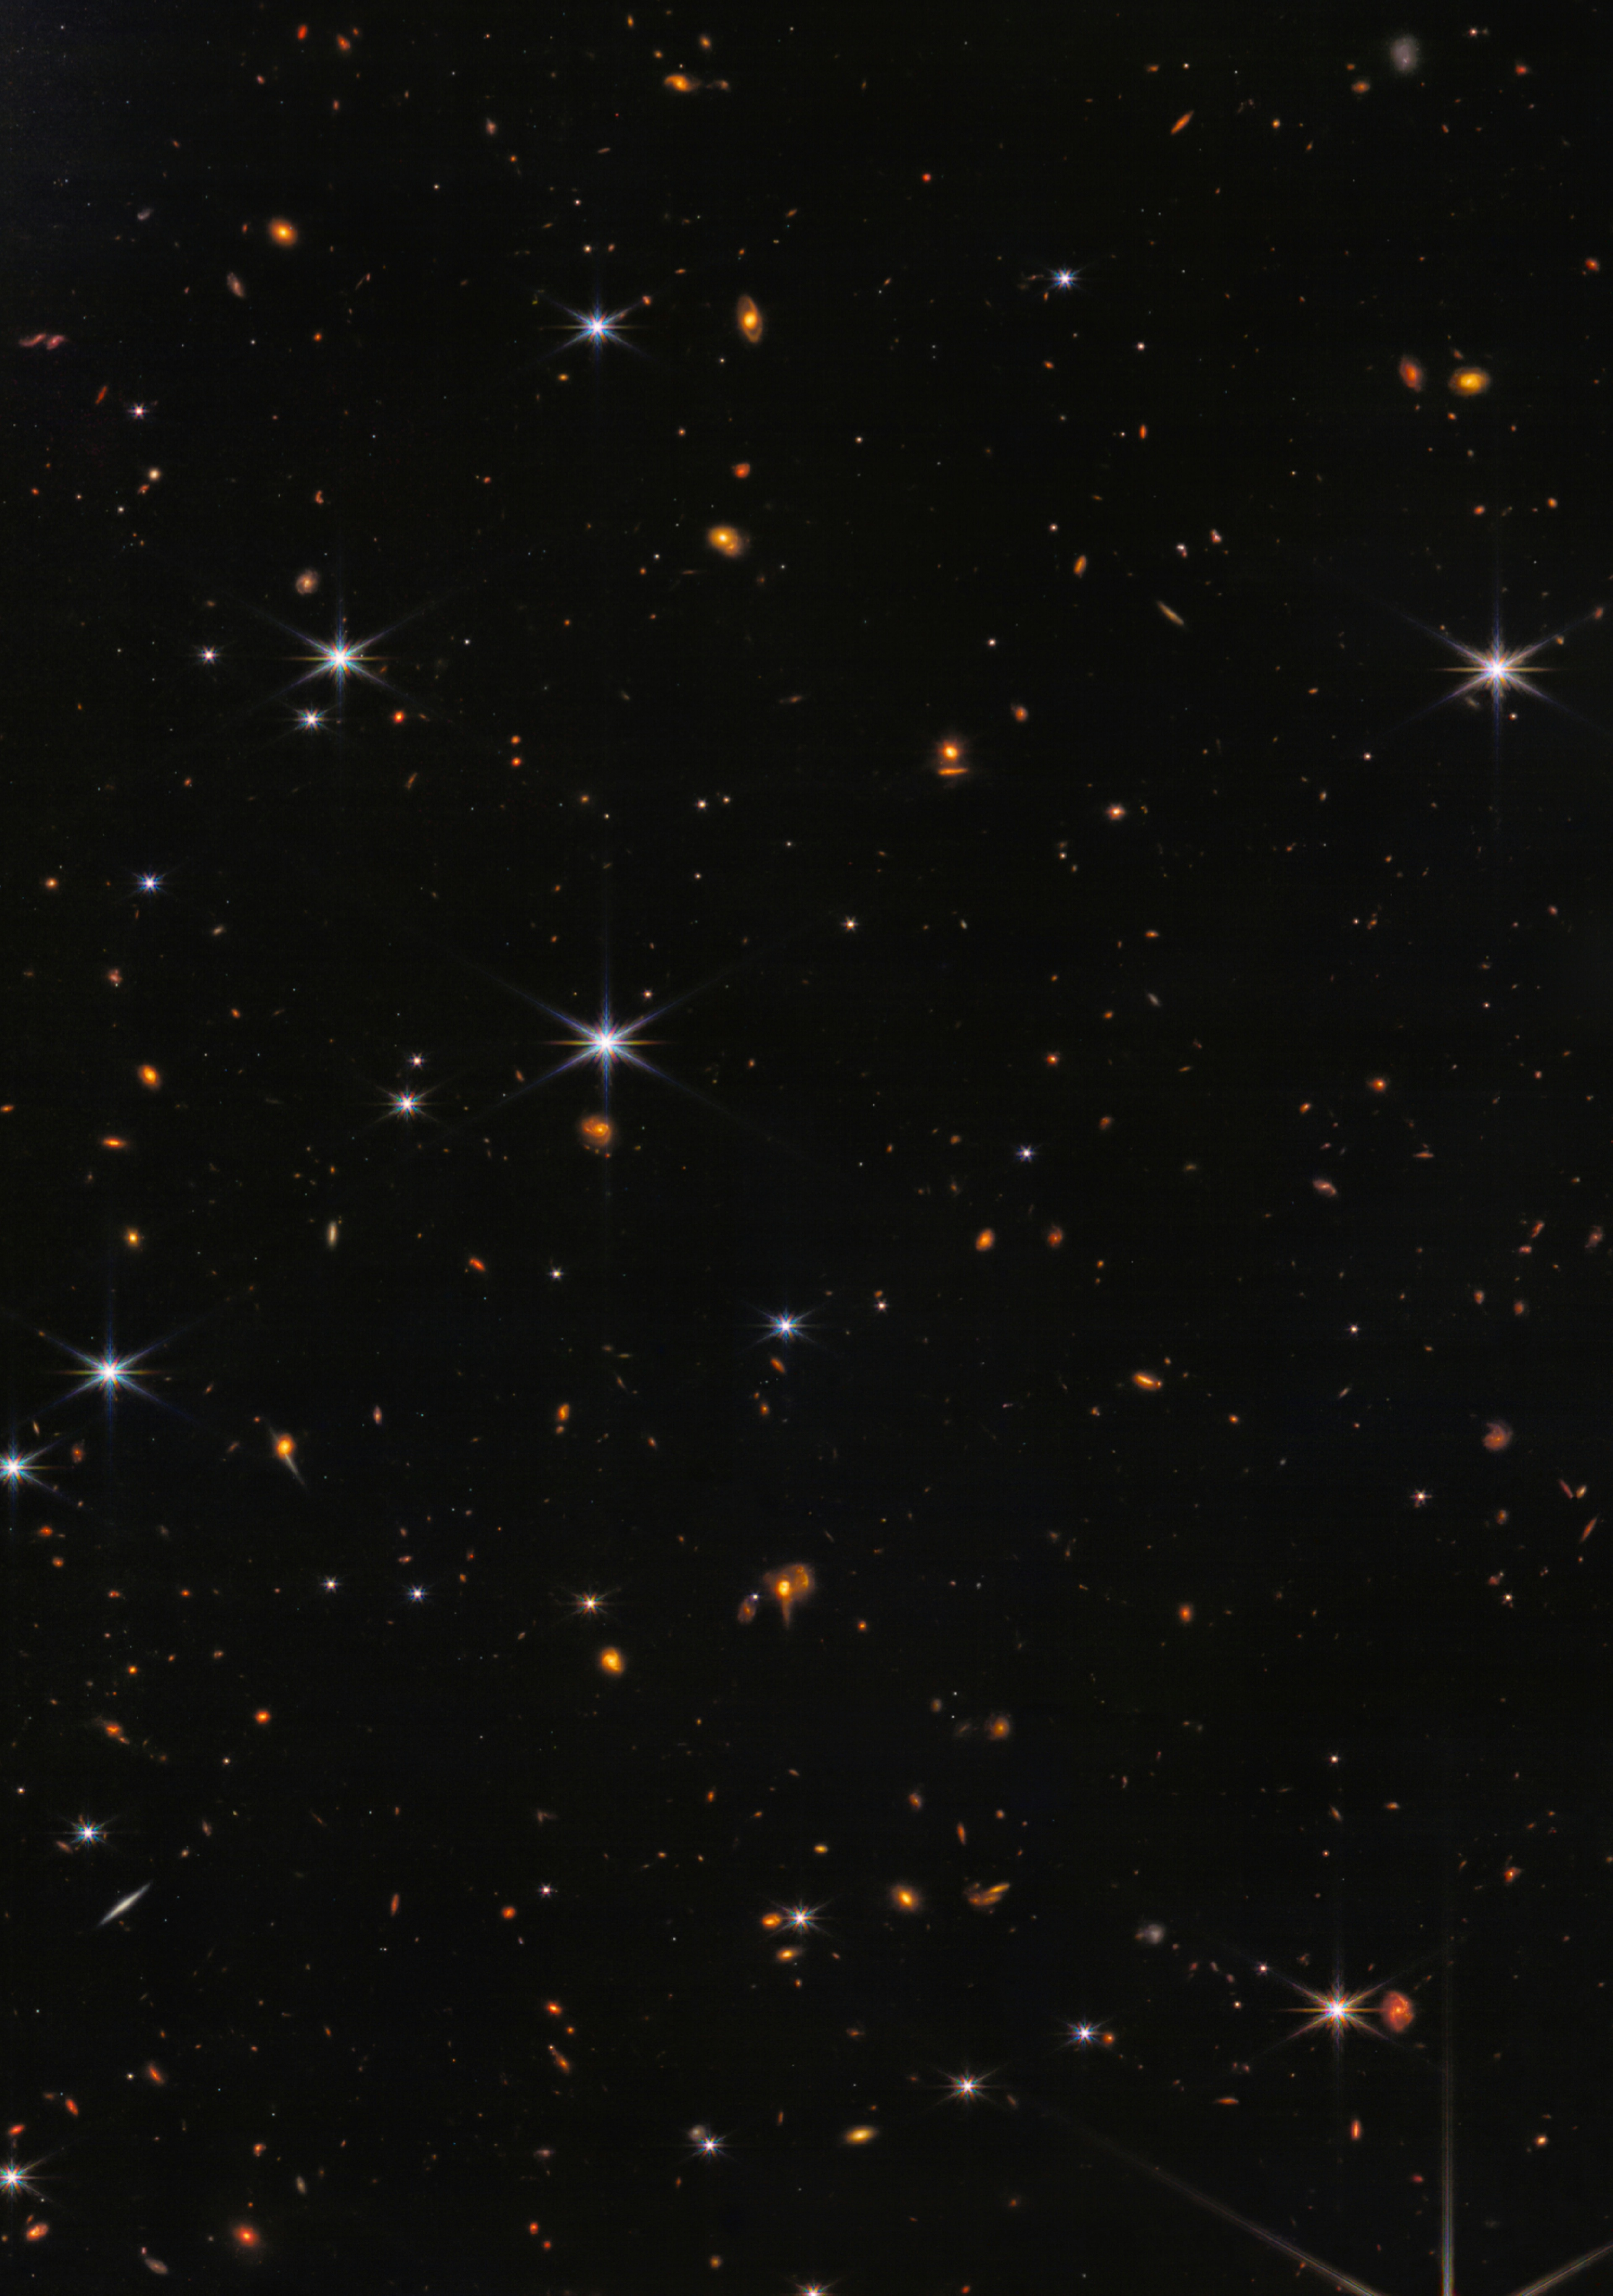
\includegraphics[width=\paperwidth,height=\paperheight,%
keepaspectratio]{images/bg.jpg}%
\vfill
}}}

\begin{document}

\color{white}
\AddToShipoutPicture*{\BackgroundPic}
\begin{titlepage}
    \begin{center}
        \vspace*{1cm}
            
        {\Huge \textbf{Summer of Science}}
            
        \vspace{0.5cm}
        {\Large Quantum Computing \& Information - P02}
            
        \vspace{1.5cm}
        \large    
        Shaik Awez Mehtab \\ \textbf{Roll No:} 23b1080 \\ \textbf{Mentor:} Kanishk Modi
            
        \vfill

        {\huge Midterm Report}
            
        \vspace{0.8cm}
            
        
\includegraphics[width=0.2\textwidth]{images/iitb_logo}
            
        \large
        IIT Bombay\\
        \today
            
    \end{center}
\end{titlepage}
\color{black}

\thispagestyle{plain}
\begin{center}
    \Large
    \textbf{Abstract}
\end{center}
In this first half of the project, I learned the basics of quantum computing and information followed by the study of quantum noise and operations, the book \ref{book:nielsen_chuang} has helped me a lot in this process and I've done most of my study from this book. Starting with linear algebra, I grasped new "quantum mechanical" notation followed by several theorems and definitions relevant to quantum mechanics like commutators, anticommutators, tensor products and polar and singular value decompositions etc. I then  built a basic foundation of quantum mechanics by learning its postulates along with density operators. Applications like superdense coding helped in gaining more insight. This was followed by an overview of quantum information and computing by studying about qubits, quantum gates, quantum circuits, the no-cloning theorem, quantum teleportation etc. I studied few quantum algorithms like Deutsch's algorithm, Deutsch-Jozsa algorithm followed by Stern-Gerlach experiment which provided an experimental overview of quantum information processing. I then studied about quantum noise and quantum operations where I first got to properly understand what "noise" means, atleast in classical sense.I then studied different approaches to understand quantum operations, most importantly operator-sum representation. This was followed by understanding few examples of quantum noise and operations using Bloch sphere, generated by bit-flip, phase-flip, bit-phase-flip, depolarizing channels. At the end, I've covered amplitude and phase damping. I wrote this report simultaneouly while I was studying, please forgive any typos.
\begin{center}
    \section*{Revised PoA}
\end{center}
\subsection*{Timeline}
\begin{itemize}
    \item \textbf{Week 5:} Distance measures for quantum information, Entropy and Information.
    \item \textbf{Week 6:} Quantum Circuits.
    \item \textbf{Week 7:} The quantum Fourier transform and its applications.
    \item \textbf{Week 8:} Quantum Search Algorithms.
\end{itemize}

\subsection*{Resources}
\begin{enumerate}[label={[\arabic*]}]
    \item MIT Open Learning Library. \href{https://openlearninglibrary.mit.edu/courses/course-v1:MITx+8.370.1x+1T2018/about}{\texttt{https://openlearninglibrary.mit.edu/course \\ s/course-v1:MITx+8.370.1x+1T2018/about}} . Quantum Information Science I, Part 1.
    \item \label{book:nielsen_chuang} \href{https://profmcruz.wordpress.com/wp-content/uploads/2017/08/quantum-computation-and-quantum-information-nielsen-chuang.pdf}{Michael A. Nielsen and Isaac L. Chuang.} \textit{Quantum Computation and Quantum Information: 10th Anniversary Edition}. Cambridge University Press, 2011.
\end{enumerate}
\tableofcontents

\part{Week 1}
\chapter{Linear Algebra}
Usual Linear algebra notation is changed to \textbf{Dirac Notation}.

We consider vector spaces in $\mathbb{C}^n$, with additive \& multiplicative properties on $\mathbb{C}^n$ too, i.e $\mathbb{C}^n$ is \textit{n} dimensional. Here, the scalars are \textbf{complex}.

\section{Dirac Notation}
A vector $\psi$ is denoted by $\ket{\psi}$\footnote{$\ket{0}$ isn't the zero vector, zero vector is denoted by just 0}
.$\ket{\psi}$ is referred to as ket, it’s vector dual $\bra{\psi} $ is referred to as bra. $\ket{\psi}$ is nothing but an n-tuple of complex numbers, $(\psi_1,\cdots, \psi_n)$ or a column vector $\begin{bmatrix} \psi_1 \\ \vdots \\ \psi_n \end{bmatrix}$

few more dirac notations:
\begin{table}[htbp]
    \centering
    \begin{tabular}{|c|p{8cm}|}\hline
        \textbf{Notation} & \textbf{Description}  \\\hline
        $z^{*}$ & Complex conjugate of z, $z \in \mathbb{C}$. eg.$(1+i)^{*} = 1-i$ \\\hline 
        $\braket{\phi | \psi}$ & Inner product (Dot product) of $\ket{\phi}$ and $\ket{\psi}$ \\\hline
        $\ket{\psi} \otimes \ket{\phi} \text{or}
\ket{\psi}\bra{\phi}$ & Outer product of $\ket{\psi}$ and $\ket{\phi}$ \\\hline
        $A^{\dagger}$ & Hermitian conjugate or Adjoint of A, = $(A^T)^*$ \\\hline
        $\braket{\psi|A|\phi}$ & Inner product between $\psi \text{ and } A\ket{\phi}$ or, Inner product between $\ket{\phi}$ and $A^{\dagger}\ket{\psi}$ \\\hline
    \end{tabular}
    \caption{Useful \textit{Dirac} notations.}
    \label{tab:dirac_notations}
\end{table}

Revise spanning set, span, linear independence, basis, dimension. They're similar to the case of real scalars.

I'll write down few important definitions from linear algebra (and few facts too):

\section{Linear Operators}

A function $A$, from vector space $V$ to $W$, which obey 

$$
A(\sum_i a_i\ket{v_i}) = \sum_i a_iA(\ket{v_i})
$$

in simpler words, operator on a linear combination of inputs is same linear combination of operator on each input

When based of inputs \& output are specified, using coordinate vectors, A linear operator is equivalent to matrix multiplication.

\subsection{Pauli Matrices}
These are 4 fundamentally important matrices in quantum information \& computation.

\begin{align*}
\sigma_0 = I = \begin{bmatrix}  1 & 0 \\ 0 & 1\end{bmatrix}
&
\sigma_1 = \sigma_x = X = \begin{bmatrix}  0 & 1 \\ 1 & 0\end{bmatrix}
\\
\sigma_2 = \sigma_y = Y = \begin{bmatrix}  0 & -i \\ i & 0\end{bmatrix}
&
\sigma_3 = \sigma_z = Z = \begin{bmatrix}  1 & 0 \\ 0 & -1\end{bmatrix}
\end{align*}

\section{Inner Products}

This is a bit different from it's real counterpart, due to the reason below.

$$
\braket{v|w} = (\ket{v},\ket{w}) = \sum_i v_i^*w_i = \begin{bmatrix}v_1^* \cdots v_n^*\end{bmatrix}\begin{bmatrix}w_1 \\ \vdots \\ w_n\end{bmatrix}
$$

the conjugate comes from the fact that this should denoted length squared (for equal vectors). the formal reason is:

Inner product between two vectors $\ket{v}$ and $\ket{w} \in V$ is a function $(.,.):V \times V\rightarrow \mathbb{C}$ which satisfies:

\begin{enumerate}    
\item $(\ket{v}, \sum_i \lambda_i\ket{w_i}) = \sum_i\lambda_i(\ket{v}, \ket{w_i})$
\item $( \ket{v}, \ket{w} ) = (\ket{w}, \ket{v})^*$
\item $(\ket{v}, \ket{v}) \geq 0, \text{0 only when} \ket{v} = 0$
\end{enumerate}

\begin{equation}
( \sum_i\lambda_iw_i , v) = \sum_i\lambda_i^*(w_i,v)
\end{equation}

Any vector space that has a defined inner product is called an \textbf{inner product space} or \textbf{Hilbert space} (if finite dimension) in QIC.

Revise orthogonality, norm, orthonormal set, gram-schmidt process. they're same as in real case.
We'll consider only orthonormal based for linear operators, and assume same spaces have same bases.

\subsection{Dual of a vector}

it would've been evident from dot product that

$$
\bra{v} = (\ket{v}^T)^*
$$

i.e if $\ket{v} = (v_1,\cdots, v_n)^T$, then

$$
\bra{v} = \begin{bmatrix}v_1^* \cdots v_n^*\end{bmatrix}
$$

\section{Outer Product}

outer product of $\ket{v} \in V$  \&  $\ket{w} \in W$ is $\ket{v}\bra{w}$

it can be seen that this is a matrix, hence it's a linear operator from W to V. let $\ket{w'} \in W$,

\begin{align*}
\underbrace{\ket{v}\bra{w}}_\text{operator}\ket{w'} =\ket{v} \underbrace{\braket{w|w'}}_\text{scalar}\end{align*}

\subsection{Completeness Relation}
Continuing from yesterday, there's this not so trivial property using outer product, called \textbf{completeness relation}

$$
\sum_i \ket{i}\bra{i} = I
$$

Here, $\ket{i}$’s form an orthonormal basis, they can be anything. one nice use of this is, if we have vector spaces V \& W, which have bases $\ket{v_1},\cdots,\ket{v_m}$ and $\ket{w_1},\cdots,\ket{w_n}$ then any linear transform $A : V \rightarrow W$ which is of size $n \times m$  can be written as a linear combination of 

$$
\ket{w_1}\bra{v_1}, \cdots,\ket{w_2}\bra{v_1},\cdots,\ket{w_n}\bra{v_m}
$$

each of which are $n \times m$. The linear combination is given by

$$
A = \sum_{ij} \underbrace{\braket{w_j|A|v_i}}_{\text{scalar}}\underbrace{\ket{w_j}\bra{v_i}}_{\text{one of the basis matrix}}
$$

eg. I can write the pauli matrix $\sigma_0$  as 

$$
1*\ket{0}\bra{0} + 0 *\ket{0}\bra{1} + \\0*\ket{1}\bra{0} + 1*\ket{1}\bra{1}
$$

\subsection{Cauchy Schwartz Inequality}

For any two vectors $\ket{v}, \ket{w}$ of same dimension, the following inequality is always true

$$
\braket{v|v}\braket{w|w} \geq \braket{v|w}\braket{w|v} = |\braket{v|w}|^2
$$

\href{https://drive.google.com/file/d/1u_q4FOFGTbASSS0xR9YSNNd0d1mMmaXg/view?usp=drive_link}{here's} a short proof I've written. $\ket{0},\cdots,\ket{n}$ are orthonormal based I've considered/can be constructed by gram schmidt process.

\section{Eigenvectors \& Eigenvalues}

it's the same as you know, just a slight change in notation. we represent both eigenvalue and eigenvector label as $v$. 

$$
\underbrace{A}_{\text{linear operator}}\ket{v} = \underbrace{v}_{\text{scalar}}\ket{v}
$$

and the characteristic function is $\text{c}(\lambda) = \text{det}(A-\lambda I)$. it depends only on the operator, not on how it's matrix is represented.

Eigenspace of an eigenvalue v is the set of vectors which have eigenvalue v. read diagonalisability, orthonormal decomposition, degenerate eigenvectors.

\section{Special Operators}
\subsection{Adjoints \& Hermitian operators}

for any linear operator $A$ on a vector space $V$$A^{\dag}$, there exists a unique linear operator $A^{\dagger}$ such that, $\forall \ket{v},\ket{w} \in V$

$$
(\ket{v}, A\ket{w}) = (A^{\dag}\ket{v},\ket{w})
$$

I've deduced that $A^\dag = (A^T)^*$  \href{https://drive.google.com/file/d/12j8H4VlHlTrKI9OzHML-qFnC_DQJ2wmV/view?usp=drive_link}{here}, when $A$ is represented as a matrix. This is actually same as dual of a vector. Few properties:

\begin{enumerate}
\item $(AB)^\dag = B^\dag A^\dag$
\item $\ket{v}^\dag = \bra{v}$
\end{enumerate}

Thus you can see $(A\ket{v})^\dag = \bra{v}A^\dag$, hence the above thing is evident.

It is \textbf{anti-linear.}

$$
\left(\sum_i a_iA_i\right)^\dag =  \sum_i a_i^*A_i^\dag
$$

A \textbf{\textit{Hermitian}} or a \textit{\textbf{self-adjoint operator}} is a linear operator such that $A^\dag = A$.

\subsection{Projectors}

these are nice. suppose $W$ is a k-dimensional subspace of $V$, which is d-dimensional, we can always construct, using \textit{gram-schmidt} process, an orthonormal basis $\ket{1},\cdots,\ket{d}$ of $V$ such that $\ket{1},\cdots,\ket{k}$ is an orthonormal basis of $W$. Now we can project any vector in $V$ onto $W$, using this operator:

$$
P = \sum_{i=1}^{k}\ket{i}\bra{i}
$$

cross check this. This operator $P$ is called the \textbf{projector}. It is also Hermitian. and we'll use $P$ to refer to $V$. $Q = I - P$ is the \textbf{orthogonal complement} of $P$.

\subsection{Normal Operators}

An operator $A$ is normal if $A^\dag A = AA^\dag$. all hermitian operators are normal.


\begin{theorem}[\textbf{Spectral Decomposition Theorem}]
    
\label{thm:spectral_decomposition}

$$
M \text{ is a normal operator on } V \iff M \text{ is diagonalisable}
$$

diagonalisable w.r.t some basis in $V$. The proof is interesting to read, do check it out.
\end{theorem}

\section{Tensor Products}
\textit{Tensor product} is a way of putting vector spaces together to form larger vector spaces. For example, if we have vector spaces $V$ and $W$ of dimension \textit{m} \& \textit{n} respectively, the tensor product $V\otimes W$ represents an \textit{mn} dimensional vector space. 

Suppose $\ket{v} \in V \ \& \ \ket{w} \in W$ be two vectors, their tensor product $\ket{v} \otimes \ket{w}$ is also represented as $\ket{v}\ket{w}, \ket{v,w}$ or even $\ket{vw}$, and it lies in \textit{mn} dimensional space $V \otimes W$

They have few nice properties:
\begin{enumerate}
    \item For a scalar $z$,
    \begin{align}
        z(\ket{v} \otimes \ket{w}) =
        (z\ket{v}) \otimes \ket{w}
    \end{align}
    \item For $\ket{v_1}, \ket{v_2} \in V$
    \begin{align}
        (\ket{v_1} + \ket{v_2}) \otimes \ket{w} = \ket{v_1} \otimes \ket{w} + \ket{v_2} \otimes \ket{w}
    \end{align}
    \item For $\ket{w_1}, \ket{w_2} \in W$
    \begin{align}
        \ket{v} \otimes (\ket{w_1} + \ket{w_2}) = \ket{v} \otimes \ket{w_1} + \ket{v} \otimes \ket{w_2}
    \end{align}
    \item 
    If we have operators $A:V\xrightarrow{}V$ \& $B:W\xrightarrow{}W$, we can define a new operator $A \otimes B : V \otimes W \xrightarrow{} V \otimes W$, we can't write it in matrix form, but we know it's a linear operator and,
    \begin{align}
        (A \otimes B)(\ket{v} \otimes \ket{w}) \equiv A\ket{v} \otimes B\ket{w}
    \end{align}
    \item We can define inner product in $V \otimes W$ as
    \begin{align}
        (a_i\ket{v_i} \otimes \ket{w_i},
        b_j\ket{v_j} \otimes \ket{w_j}) = a_i^*b_j \braket{v_i|v_j}\braket{w_i|w_j}
    \end{align}
    As we have a well defined inner product, this is a hilbert space too, we can use properties like adjoint, unitary, normal, hermitian matrices.

    \subsection{Kronecker Product}
    There is indeed a representation which would let us interpret tensor product in some manner, suppose we have two matrices $A_{m\times n}, B_{p \times q}$,
    their tensor product in this representation is:
    \begin{equation}
        A \otimes B =
        \begin{bmatrix}
            A_{11}B & A_{12}B & \cdots & A_{1n}B \\
            A_{21}B & A_{22}B & \cdots &
            A_{2n}B \\
            \vdots & \vdots & \vdots & \vdots \\
            A_{m1}B & A_{m2}B & \cdots & A_{mn}B
        \end{bmatrix}_{mp \times nq}
    \end{equation}

    for example, tensor product of Pauli matrices $X$ \& $Y$ is represented as
    \begin{equation}
        X \otimes Y =
        \begin{bmatrix}
            0\cdot Y & 1\cdot Y \\
            1\cdot Y & 0\cdot Y
        \end{bmatrix}
        =
        \begin{bmatrix}
            0 & 0 & 0 & -i \\
            0 & 0 & i & 0 \\
            0 & -i & 0 & 0 \\
            i & 0 & 0 & 0
        \end{bmatrix}
    \end{equation}
    and another example, 
    \begin{equation}
        \begin{bmatrix}
            1 \\ 2
        \end{bmatrix}
        \otimes
        \begin{bmatrix}
            2 \\ 3
        \end{bmatrix}
        = 
        \begin{bmatrix}
            2 \\ 3 \\ 4 \\ 6
        \end{bmatrix}
    \end{equation}
    Using similar notations, $\ket{\phi}^{\otimes k}$ means tensor product of $\ket{\phi}$ with itself k times.
\end{enumerate}

Just for practice, I'm writing down few tensor products, $I,X,Y,Z$ are pauli matrices.
\begin{align}
    X \otimes Z &= 
    \begin{bmatrix}
        0 & 0 & 1 & 0 \\
        0 & 0 & 0 & -1 \\
        1 & 0 & 0 & 0 \\
        0 & -1 & 0 & 0
    \end{bmatrix} &
    I \otimes X &=
    \begin{bmatrix}
        X & 0 \\ 0 & X
    \end{bmatrix}
    = 
    \begin{bmatrix}
        0 & 1 & 0 & 0 \\
        1 & 0 & 0 & 0 \\
        0 & 0 & 0 & 1 \\
        0 & 0 & 1 & 0
    \end{bmatrix}
\end{align}
\begin{align}
    X \otimes I &=
    \begin{bmatrix}
        0 & 0 & 1 & 0 \\
        0 & 0 & 0 & 1 \\
        1 & 0 & 0 & 0 \\
        0 & 1 & 0 & 0
    \end{bmatrix}
\end{align}
Hence, tensor product \textbf{isn't commutative}.
Few more facts,
\begin{enumerate}
    \item $(A \otimes B)^* = A^* \otimes B^*$
    \item $(A \otimes B)^T = A^T \otimes B^T$
    \item $(A \otimes B)^\dag = A^\dagger \otimes B^\dagger$
    \item Tensor product preserves 
    \begin{enumerate*}
        \item Unitarity
        \item Hermiticity
        \item Positivity
        \item Projection
    \end{enumerate*}
\end{enumerate}

\section{Operator functions}
If we have a function $f : \mathbb{C}^n \rightarrow \mathbb{C}^n$, we can define a corresponding matrix function, which acts on \textit{normal matrices} as follows

\begin{equation}
    A = \sum_a a\ket{a}\bra{a} \implies
    f(A) \equiv \sum_a f(a)\ket{a}\bra{a}
\end{equation}

where $\sum_a a\ket{a}\bra{a}$ is a spectral decomposition (exists since A is normal \ref{thm:spectral_decomposition}). Now we can calculate square root, logarithm, exponential of a positive, positive-definite, normal operator respectively.
for eg.
\begin{equation}
    \exp{(\theta Z)} =
    \begin{bmatrix}
        e^\theta  & 0 \\
        0 & e^{-\theta}
    \end{bmatrix}
\end{equation}

I'll do another example, let $A = \begin{bmatrix}
    4 & 3 \\ 3 & 4
\end{bmatrix}$, let's find square root of it.
Eigenvalues of A are 7, 1. Their corresponding eigenvectors which form an orthonormal basis of $\mathbb{R}^2$ are $(\ket{0} + \ket{1})/\sqrt{2} = \ket{a}$ \& $(\ket{0}-\ket{1})/\sqrt{2} = \ket{b}$,
\begin{align}
    A &= 7\ket{a}\bra{a} + \ket{b}\bra{b} \\
    \implies \sqrt{A} &= \sqrt{7}\ket{a}\bra{a} + \ket{b}\bra{b} \\
    &= \begin{bmatrix}
        \frac{\sqrt{7} + 1}{2} & \frac{\sqrt{7}-1}{2}\\
        \frac{\sqrt{7}-1}{2} & \frac{\sqrt{7} + 1}{2} 
    \end{bmatrix}
\end{align}

\subsection{Trace}
This is just the sum of diagonal elements of a matrix. 
% \newcommand{\tr}[1]{\text{tr}(#1)}
\begin{equation}
    \tr{A} = \sum_i A_{ii}
\end{equation}
It's also defined as
\begin{equation}
    \tr{A} = \sum_i \braket{i|A|i}
\end{equation}
i.e it doesn't depend on which coordinate I represent A on, traces have these nice properties:
\begin{enumerate}
    \item It's \textit{cyclic}, $\tr{AB} = \tr{BA}$
    \item $\tr{cA + dB} = c\tr{A} + d\tr{B}, c,d \in \mathbb{C}$
    \item if $U$ is unitary, $\tr{A} = \tr{UAU^{\dag}}$   
    \item $\tr{A\ket{\psi}\bra{\psi}} = \braket{\psi|A|\psi}$
\end{enumerate}

\subsection{Hilbert-Schmidt inner product}
The vector space $L_V$ of linear operators on a Hilbert space $V$ can be converted into a Hilbert space by defining an inner product on $L_V \times L_V$ as
\begin{equation}
    (A, B) \equiv \tr{A^\dag B}
\end{equation}
this is known as the \textit{Hilbert-Schmidt} or \textit{Trace} inner product.

\section{Commutator \& Anti-commutator}

The commutator between two operators $A$ \& $B$ is defined as
\begin{equation}
    [A, B] = AB - BA
\end{equation}
if $[A, B] = 0 \implies AB = BA$, then we say $A$ \textit{commutes} with $B$. The \textit{anti-commutator} between $A$ \& $B$ is defined as
\begin{equation}
    {A, B} = AB + BA
\end{equation}
we say $A$ \textit{anti-commutes} with $B$ if {A, B} = 0.

\begin{theorem}[\textbf{Simultaneous diagonalization theorem}]
    If $A$ \& $B$ are Hermitian operators, then
    $[A, B] = 0 \implies \exists$ an orthonormal basis such that both $A$ and $B$ are \textit{simultaneously diagonalizable} w.r.t same basis.
\end{theorem}

\subsubsection{Commutations \& Anti-commutation for Pauli matrices}
\begin{align}
    [X, Y] &= 2iZ & [Y,Z] &= 2iX & [Z,X] &= 2iY \\
\end{align}
we can write it using $\epsilon_{jkl}$, the antisymmetric tensor, for which $\epsilon_{jkl} = 0$ except for $\epsilon_{123} = \epsilon_{231} = \epsilon_{312} = 1$ and $\epsilon_{321} = \epsilon_{213} = \epsilon_{132} = -1$:
\begin{align}
    [\sigma_j, \sigma_k] = 2i\sum_{i=1}^3 \epsilon_{jkl}\sigma_l
\end{align}
Also, $\{\sigma_i, \sigma_j\} = 0, \forall i\neq j, i.j \in {1,2,3}$. whereas $\{\sigma_0, \sigma_j\} = 2\sigma_j$. 

\section{Polar and Singular value decompositions}
\begin{theorem}[\textbf{Polar decomposition}]
    Let $A$ be a linear operator on a vector space $V$. Then there exist unitary $U$ and \textbf{positive operators} $J$ and $JK$ such that
    \begin{equation}
        A = UJ = KU
    \end{equation}
    where the unique positive operators $J$ \& $K$ are $J \equiv \sqrt{A^\dag A}$ and $K \equiv \sqrt{AA^\dag}$, if $A$ is invertible, $U$ is unique.
\end{theorem}
$A=UJ$ is the left polar decomposition of $A$, and $A=KU$ is the right polar decomposition of A

Singular value decomposition is just polar decomposition \& spectral decomposition.
\begin{corollary}[\textbf{Singular value decomposition}]
    Let A is a square matrix, Then $\exists$ unitary $U\ \& \ V$, a diagonal matrix $D$ with \textbf{non-negative entries} such that
    \begin{align}
        A = UDV
    \end{align}
    diagonal elements of D are called \textbf{singular values} of A.
\end{corollary}
\begin{proof}
    By polar decomposition, A = SJ, where S is unitary and J is positive.  By spectral decomposition, $J = TDT^\dag$ where T is unitary and D has non negative entries. setting $U=ST$ and $V=T^\dag$ we get the above thing.
\end{proof}
\chapter{Postulates of Quantum Mechanics}

\section{State Space}

\begin{postulate}
    Any isolated physical system has a Hilbert Space associated with it known as the \textbf{state space}. The system is completely described by it's \textbf{state vector}, which is a unit vector in state space.
\end{postulate}

The simplest quantum mechanical system, which we'll be concerned the most about, is a \textit{qubit} which has a 2-dimensional state space. Hence an arbitrary state vector $\ket{\psi}$ can be represented by

\begin{equation}
    \ket{\psi} = \alpha \ket{0} + \beta \ket{\psi}
\end{equation}

where $\alpha, \beta \in \mathbb{C}$ and $\ket{0}, \ket{1}$ form an orthonormal basis of state space. Since state vector is a unit vector, $\braket{\psi|\psi} = 1 \implies |\alpha|^2 + |\beta|^2 = 1$, this is known as \textit{normalization} of state vector.

For now, \textit{qubit} is an abstract thing. We consider a fixed orthonormal basis $\ket{0}, \ket{1}$ apriori. These two states can be considered analogous to the bits 0 and 1, except that a state vector is a linear combination, or in other words, \textit{superposition } of these bits. The linear combination $\sum_i \alpha_i \ket{\psi_i}$ is defined as the superposition of $\ket{\psi_i}$ with amplitude $\alpha_i$ for $\ket{\psi_i}$.


\section{Evolution}

\begin{postulate}
    The evolution of a \textbf{closed} system is described by a \textbf{unitary transformation}. The state of the system $\ket{\psi}$ at time $t_1$ is related to the state of the system $\ket{\psi^{'}}$ at time $t_2$ solely by the unitary transformation U which only depends on $t_1, t_2$

    \begin{equation}
        \ket{\psi^{'}} = U\ket{\psi}
    \end{equation}
    \label{postulate_2}
\end{postulate}

Quantum mechanics doesn't help us find the \textit{state space} or \textit{unitary operator}, it just assures us that any physical system would behave this way.

Few such operator on a qubit are pauli matrices. X is referred to as \textit{NOT gate} or \textit{bit-flip} since it turns $\ket{0}$ to $\ket{1}$ and vice versa. Z is known as \textit{phase-flip} as it leaves $\ket{0}$ as it is, which inverting the phase (sign) of $\ket{1}$.

The second postulate just defines state of the system at discrete intervals $t_1$ and $t_2$, this can be generalised for \textit{continuous} t.
\begin{corollary}
    Time evolution of a \textbf{closed} quantum system is described by \textbf{Schrödinger equation},
    \begin{equation}
        i\hbar \frac{d\ket{\psi}}{dt}
        = H\ket{\psi}
    \end{equation}
    where $\hbar$ is the reduced planck's constant, H is a fixed \textbf{Hermitian} operator known as the \textbf{Hamiltonian} of the closed system.
    \label{schrodinger_eq}
\end{corollary}

Since Hamiltonian is a Hermitian operator, it has a spectral decomposition,
\begin{equation}
    H = \sum_E E\ket{E}\bra{E}
\end{equation}

Here the eigenvectors $\ket{E}$ are conventionally called \textit{energy eigenstates} or \textit{stationary states} and $E$ is called \textit{energy} of the state $\ket{E}$. The lowest energy is known as \textit{ground state energy} and the corresponding state is the \textit{ground state.}

We can see a connection between corollary \ref{postulate_2} and postulate \ref{schrodinger_eq}, if we know the solution of Schr\"{o}dinger's equation, which can be verified that it is

\begin{equation}
    \ket{\psi(t_2)} = exp\left[\frac{-iH(t_2-t_1)}{\hbar}\right]\ket{\psi(t_1)} = U(t_1,t_2)\ket{\psi(t_1)}
\end{equation}

if we set, 
\begin{equation}
    U(t_1,t_2) \equiv exp\left[\frac{-iH(t_2-t_1)}{\hbar}\right]
\end{equation}

it can be shown that if $K$ is a Hermitian operator, then $U=exp(iK)$ is a unitary operator. Thus, there's a one-to-one correspondence between the theorem and it's corollary.

If the system we're considering is not closed, we can approximate it's evolution using a time varying Hamiltonian. There's this example that when we consider a laser focused on an atom, the whole system is properly described by a Hamiltonian, but the behaviour of the atome alone, is seem to be approximately described by another Hamiltonian, this thing contains terms related to the laser intensity.

\section{Quantum measurement}

We've seen that in closed systems, the evolution of state vector is according to a unitary transform, but when we try to measure the state of the system, we need to interact with it, which leads to a change other than a unitary transform, which is described as

\begin{postulate}
    A \textbf{quantum measurement} is a collection $\{M_m\}$ of measurement operators. These operators act on the state space. The index m refers to the measurement outcome that we want using $M_m$. If the system is in state vector $\ket{\psi}$ before the measurement had been made, the probability that outcome is m is,
    \begin{equation}
        \label{eq:measurement_probability}
        p(m) = \bra{\psi}M_m^\dag M_m\ket{\psi}
    \end{equation}
    After the measurement, the state changes to
    \begin{equation}
        \frac{M_m\ket{\psi}}{\sqrt{\bra{\psi}M_m^\dag M_m\ket{\psi}}}
    \end{equation}
    All the $M_i$ satisfy the \textbf{completeness relation}
    \begin{equation}
        \sum_i M_i^\dag M_i = I
    \end{equation}
    This ensures the probability that some measurement occurs is 1,
    \begin{equation}
        \sum_i p(i) = \sum_i \bra{\psi}M_i^\dag M_i\ket{\psi} = 1
    \end{equation}
\end{postulate}

As an example, suppose we have a closed system whose state vector $\ket{\psi}$ is currently $a\ket{0} + b\ket{1}$ and we want to make measurements using $M_0 = \ket{0}\bra{0}$ and $M_1 = \ket{1}\bra{1}$, we can calculate and see that probability that measurements 0 \& 1 are made correct are $|a|$ and $|b|$ respectively, and the final states are
$\frac{a}{|a|}\ket{0}$ if we make measurement 0 and $\frac{b}{|b|}\ket{1}$ if we make measurement 1.

So when there's an isolated physical system, it has a state vector, when you try to measure it, using the collection of measurement operators gives just a label. we can just get the probability that we get a specific probability, using equation \ref{eq:measurement_probability}

\section{Distinguishing quantum states}
When we have $n$ systems, with $n$ state vectors, we can only distinguish them by measuring them only if all the state vectors are orthonormal. This has a good proof.

\begin{theorem}
    No measurement distinguishing non-orthogonal states is possible
\end{theorem}

\begin{proof}
    We consider two states $\ket{\psi_1}, \ket{\psi_2}$ and assume that there exists a measurement. We distinguish these states by looking at the output label we get from the measurement. Taking the function $f(j)$ where $j$ is the label. If the state is $\ket{\psi_1}$ then probability that our prediction is correct $\sum_{j; f(j)=1} \bra{\psi_1}M_j^\dag M_j \ket{\psi_1} = 1$ similarly for 2. To simlify this we define

    \begin{equation}
        E_i = \sum_{j; f(j) = i} M_j^\dag M_j
    \end{equation}
    so from what we've done above
    \begin{align}
        \bra{\psi_1}E_1\ket{\psi_1} = 1 &
        \bra{\psi_2}E_2\ket{\psi_2} = 1
    \end{align}
    since we'll always measure $\ket{\psi_1}$'s label when the state is $\ket{\psi_1}$,
    \begin{align}
        \bra{\psi_1}E_2\ket{\psi_2} &= 0 \\
        \implies \sqrt{E_2}\ket{\psi_2} &= 0
    \end{align}
    now let's focus on the orthogonal component of $\ket{\psi_2}$, by writing it as $\ket{\psi_2} = \alpha \ket{\psi_1} = \beta \ket{\phi}$, where $\ket{\phi}$ is orthonormal to $\ket{\psi_1} \implies 
    |\beta| < 1$, since they're non-orthogonal.

    But there's a contradiction,
    \begin{align}
        \bra{\psi_2}E_2\ket{\psi_2} &=
        \beta^2 \bra{\phi}E_2\ket{\phi} \\
        &\leq |\beta|^2 \\
        &< 1 
    \end{align}
    Thus by contradiction, our assumption is false $\implies$ we can't distinguish non-orthogonal states reliably.
\end{proof}

\section{Projective measurements}
This is the main thing we'll deal in quantum information and computation.

\begin{postulate}
    A projective measurement is an observable M, a Hermitian operator on the state space of system considered, having spectral decomposition
    \begin{equation}
        M = \sum_m mP_m
    \end{equation}
    where m is one of the possible outcomes. m is an eigenvalue of $M$, $P_m$ is the projector onto the corresponding eigenspace. When we measure a state $\ket{\psi}$, the probability of getting the result m is
    \begin{equation}
        p(m) = \bra{\psi}P_m\ket{\psi}
    \end{equation}
    After measuring, the state of the system becomes
    \begin{equation}
        \frac{P_m\ket{\psi}}{\sqrt{p(m)}}
    \end{equation}
\end{postulate}

We can see projective measurement is a special kind of measurement, which do obey completeness relation, i.e $\sum_m M_m^\dag M_m = I$. But $M_m$ also are \textit{Orthogonal projectors}, hence \textit{Hermitian} and $M_mM_{m^`} = \delta_{mm^`}M_m$

These have few nice properties, we can find mean of measurements easily, which is
\begin{align}
    E(M) &= \sum_m m p(m) \\
    &= \sum_m m\bra{\psi} P_m \ket{\psi} \\
    &= \bra{\psi} \sum_m mP_m \ket{\psi} \\
    &= \bra{\psi}M\ket{\psi}
\end{align}

this is a nice thing, we can also find the standard deviation of the outcomes we get.

\begin{align}
    \Delta(M) &= \sqrt{\braket{(M-\braket{M}}^2} \\
    &= \sqrt{\braket{M^2} - \braket{M}^2}
\end{align}

As you might have observed, we defined a new term \textit{observable}, some still like to look at the projection measurement as a collection of operators, using the observable implicitly. Another phrase used is "measure in basis $\ket{m}$", which means the projectors $P_m = \ket{m}\bra{m}$ are used for projective measurement.

If $\vv{v}$ be a three dimensional unit vector, then the measurement of the observable
\begin{equation}
    \vv{v}\cdot \vv{\sigma} = v_1\sigma_1 + v_2\sigma_2 + v_3\sigma_3
\end{equation}
is historically known as the "\textit{measurement of spin along $\vv{v}$ axis}"

\begin{remark}
    Eigenvalues of $\vv{v}\cdot\vv{\sigma}$ are $\pm 1$ and the corresponding projection operators are $P_{\pm} = \frac{I \pm \vv{v}\cdot\vv{\sigma}}{2}$
\end{remark} 

\subsection{Heisenberg Uncertainty Principle}
Suppose $A$, $B$ be two Hermitian operators and $\ket{\psi}$ is a quantum state. Let $\bra{\psi}AB\ket{\psi} = x+iy$ where $x, y \in \mathbb{R}$. Then $\bra{\psi}[AB]\ket{\psi} = 2iy$ and $\bra{\psi}\{AB\}\ket{\psi} = 2x$, therefore

\begin{equation}
    \left( \bra{\psi}[A,B]\ket{\psi} \right)^2 + 
    \left( \bra{\psi} \{A,B\} \ket{\psi} \right)^2 = 
    4\left| \bra{\psi} AB \ket{\psi} \right|^2
\end{equation}
Using Cauchy-Schwartz inequality, then substituting $A = C - \braket{C}$ and $B = D-\braket{D}$
\begin{align}
    \inbk{A^2}\inbk{B^2} &\geq \left(\inbk{AB}\right)^2 \\
    &\geq \frac{\left( \inbk{[A, B]} \right)^2}{4} \\
    \implies \Delta(C)\Delta(D) &\geq
    \frac{\inbk{[C, D]}}{2}
\end{align}
Hence Proved.

Note that the common misconception of Heisenberg uncertainity principle is
that we "measure a state with some error" which is $\Delta(C), \Delta(D)$, but the actual thing is we have a large amount of $\qv$'s and we measure each of them seperately to with observables $C, D$ to get a set of values of $C, D$ whose standard deviation is $\Delta(C), \Delta(D)$. This is because once we make a measurement, the quantum state changes because we've altered it.

\section{POVM measurements}
It stands for \textit{Positive Operator-Valued Measure}. POVM is a formalism, and is used when we are concerned with the outcome more than the state of the output we're measuring. For eg. when we've done an experiment and just want to measure the final state.

If we're measuring a state $\qv$ using measurement operators $M_m$, the probability that the output is $m$ is $\inbk{M_m^\dag M_m}$, if we define
\begin{equation}
    E_m = M_m^\dag M_m
\end{equation}
$E_m$ satisfy $\sum_m E_m = I$, $E_m$ is enough to find the probability of output $m$
which is $\inbk{E_m}$. The set $\{E_m\}$ is called the \textit{POVM set}.

In projective measurements POVM set is same as the set of measurement operators, since $E_m = P_m^\dag P_m = P_m$. In fact any measurement where the measurement operators and the POVM elements coincide is a projective measurement.

If we want the post-measurement state, we can conveniently \textit{define} a POVM to be any set of operators $\{E_m\}$ such that \begin{enumerate*}[label=(\alph*)]
    \item each $E_m$ is positive
    \item it satisfies \textit{completeness relation}, i.e $\sum_m E_m = I$
\end{enumerate*}
In this way we can choose $M_m = U_m\sqrt{E_m}$ where $U_m$ is a unitary operator.

\section{Phase}
This is kind of interesting and deja vu giving.
\subsection{Global Phase}
If $\qv$ is a state, $\theta \in \mathbb{R}$, we say that $e^{i\theta}\qv$ is equal to $\qv$ upto the \textit{global phase factor $e^{i\theta}$}. These two act quite similar when you try to measure them, because the output of m would occur with a probability of $\inbk{M_m^\dag M_m}$ and $\inbk{e^{-i\theta}M_m^\dag M_m e^{i\theta}} = \inbk{M_m^\dag M_m}$, which is the same.
Thus, they're physically equivalent.

\subsection{Relative Phase}
If two amplitudes, $a$ and $b$, \textit{differ by a relative phase} if there is a real $\theta$ such that $a = be^{i\theta}$. Two states \textit{differ by a relative phase} in \textit{some basis} if each of the amplitudes in that basis is related by such a phase factor.
Unlike global phase factors, relative phase factors differ from amplitude to amplitude, thus, there are physically observable differences in measurement statistics, and two states differing by a relative phase aren't physically equivalent.

\section{Composite systems}
It's useful in describing state of a composite system made up of multiple systems 

\begin{postulate}
    The state space of a composite physical system is the tensor product of state spaces of component physical systems. If n physical systems are prepared in state $\ket{\psi_1},\cdots,\ket{\psi_n}$
    The composite system has the state $\ket{\psi_1}\otimes\ket{\psi_2}\otimes\cdots\otimes\ket{\psi_n}$
\end{postulate}

Using this, we can prove a fact.
\begin{remark}
    To implement a general measurement, it is sufficient to make projective measurements together with unitary dynamics
\end{remark}
I'm not giving the entire proof. but assume that the state space we're considering is $Q$ and we want to measure using operators $M_m$. We can consider a new \textit{ancilla} system which has state space $M$. $M$ has orthonormal basis $\ket{m}$ which are in one-to-one correspondence with the first output. Let's define an operator $U:QM \xrightarrow{} QM$ as
\begin{equation}
    U\qv\ket{0} = \sum_m M_m\qv\ket{m}
\end{equation}
where $\ket{0}$ is some state in $Q$. It can be shown that $U$ preserves dot product. i.e $\bra{0}\bra{\phi}U^\dag U \qv\ket{0} = 
\braket{\phi | \psi}$ which implies that U extends over $Q\otimes M$ which can be proved too.

Now, if we consider two systems with projectors $P_m = I_Q\otimes \ket{m} \bra{m}$ and measure using unitary dynamics and projective transformation, the probability of output $m$ is
\begin{align}
    p(m) &= \bra{\psi}\bra{0}U^\dag P_m U \ket{0}\ket{\psi} \\
    &= \sum_{m', m''}\bra{\psi}\bra{m'}M_{m'}^\dag (I_Q \otimes \ket{m}\bra{m})M_{m''}\ket{m''}\ket{\psi}\\
    &= \braket{\psi|M_m^\dag M_m | \psi}
\end{align}
which is just as measured directly from general measurement.
also the state of the composite system after the measurement is
\begin{align}
    \frac{P_mU\ket{\psi}\ket{0}}{\sqrt{\braket{
    \psi | U^\dag P_m U | \psi}
    }}
    =
    \frac{M_m\ket{\psi}\ket{m}}{
    \sqrt{
    \braket{\psi|M_m^\dag M_m | \psi}
    }
    }
\end{align}
Since the state of the system M after measurement is $\ket{m}$, state of system Q is
\begin{align}
    \frac{M_m\ket{\psi}}{\sqrt{
    \braket{\psi|M_m^\dag M_m | \psi}
    }}
\end{align}
also as measured directly from general measurement.

\subsection*{Quantum Entanglement}
This is something you would've heard of before. Consider the two qubit state,
\begin{align}
    \qv = \frac{\ket{00} + \ket{11}}{\sqrt{2}}
\end{align}
we can never write it as a tensor product of two other qubit states, i.e $\qv = \ket{a}\ket{b}$ can never be true. It's easily checkable. A state of a composite system like this, which can't be written as tensor product of it's component systems is an \textit{entangled} state. Entangled states play a cruicial rules in quantum computation and information.

\section{Application: Superdense Coding}
This nicely uses the idea of entanglement and "applying" quantum gates.
Suppose we have 'Alice' and 'Bob' again, who're away from each other. Alice wants two share two classical bits of information using one qubit to bob, can she do it?

\begin{center}
\begin{tikzpicture}
[
place/.style = {rectangle,draw=black!50,fill=black!5,
inner sep=2mm, rounded corners}
]
 \node[place] (alice) at (-4,0)  {
 \begin{minipage}{3cm}
 \centering
 Alice \\
 \vspace{3mm}
 \begin{tabular}{cc}
     00 : I & 01 : Z \\ 
     10 : X & 11 : iY
 \end{tabular}
 \end{minipage}
 };
 \node[place] (bob) at (4,0) {Bob};
 \draw [<->] (alice) -- (bob) node[midway, above] {\Large$
 \frac{\ket{00}+\ket{11}}{2}
 $}
 node[pos = 0.15, below] {
 \scriptsize
   One qubit
 }
 node[pos = 0.85, below] {
   \scriptsize
   One qubit
 };
\end{tikzpicture}
\end{center}

Yes, using superdense coding. Here, Alice and Bob share a pair of externally setup qubits in entangled state
\begin{equation}
   \qv =  \frac{\ket{00}+\ket{11}}{2}
\end{equation}
Alice has one qubit, which she can alter and Bob has another. Any change Alice makes to her qubit changes the composite system, which can be measured by Bob. So she applies quantum gates to change the qubits, as given in the diagram, which result in the following changes.

\begin{align}
    00 &: \qv \xrightarrow{I} \frac{\ket{00}+\ket{11}}{2} \\
    01 &: \qv \xrightarrow{Z}
    \frac{\ket{00}-\ket{11}}{2} \\
    10 &: \qv \xrightarrow{X}
    \frac{\ket{10}+\ket{01}}{2} \\
    11 &: \qv \xrightarrow{iY}
    \frac{-\ket{10}+\ket{01}}{2}
\end{align}

We can see that all the outputs are orthonormal, hence Bob can choose appropriate measurement operators and clearly distinguish each state, hence getting the information Alice had sent him.
These are known as the \textit{Bell states, Bell basis} or \textit{EPR pairs}.

Thus, a single qubit can be used to transfer information which would've taken two classical bits.

\section{The density operator}
Till now we've been using the language of state vectors. The density operator is a different way of representing states, it's mathematically equivalent to state vectors. It's much more convenient to use in some scenarios. It's really useful while describing \textit{individual subsystems} of a composite system.

\subsection{Ensembles of quantum states}
It's useful when we don't exactly know the state of a system. If the possible states are $\ket{\psi_i}$ with probabilities $p_i$, $\{p_i, \ket{\psi_i}\}$ is an \textit{ensemble of pure states}. The density operator, also called as the \textit{density matrix} is defined as
\begin{equation}
    \rho \equiv \sum_i p_i \op{\psi_i}
\end{equation}

We can now workout rewriting the postulates of quantum mechanics. 

Suppose, the evolution of closed quantum system is described by a unitary operator $U$. The system is initially in the state $\ket{\psi_i}$ with probability $p_i$, after the evolution, system will be in the state $U\ket{\psi_i}$ with probability $p_i$, then the density operator evolves into

\begin{equation}
    \rho = \sum_i p_i\op{\psi_i} 
    \xrightarrow{U}
    \sum_i p_i U\op{\psi_i}U^\dag
    = U\rho U^\dag.
\end{equation}

We can also predict the probability of a measurement outcome $m$, when our system is defined by the density operator $\rho$, if the initial state was $\ket{\psi_i}$, then the probabililty of outcome $m$ is

\begin{equation}
    p(m|i) = \braket{\psi_i |M_m^\dag M_m| \psi_i}
    = \text{tr}(M_m^\dag M_m \op{\psi_i})
\end{equation}

This is the probability that the outcome would be $m$, if the state was $\ket{\psi_i}$ which has a probability of $p_i$, hence the overall probability of outcome being m is
\begin{align}
    p(m) &= \sum_i p(m|i)p_i \\
    &= \sum_i p_i\text{tr}(M_m^\dag M_m\op{\psi_i}) \\
    &= \text{tr}(M_m^\dag M_m \rho)
\end{align}
Also we can find out the state of the system if the outcome was m, if the state was initially $\ket{\psi_i}$ which has probability $p_i$ the final state would be
\begin{equation}
    \ket{\psi_i^m} = \frac{M_m\ket{\psi_i}}{
    \sqrt{\braket{\psi_i | M_m^\dag M_m | \psi_i}}
    }
\end{equation}
Hence, the final density operator would be
\begin{equation}
    \rho_m = \sum_i p(i|m)\op{\psi_i^m} = 
    \sum_i p(i|m)\frac{M_m\op{\psi_i}M_m^\dag}{\braket{
    \psi_i| M_m^\dag M_m |\psi_i
    }}
\end{equation}
By Bayes' theorem, $p(i|m) = p(m|i)p_i/p(m)$, subsituting this,
\begin{align}
    \rho_m &= \sum_i p_i \frac{M_m\op{\psi_i}M_m^\dag}{\text{tr}(M_m^\dag M_m \rho)} \\
    &= \frac{M_m\rho M_m^\dag}{\text{tr}(M_m^\dag M_m \rho)}
\end{align}

A system whose state $\qv$ is exactly known is said to be in \textit{pure state}. The density operator is then simply $\op{\psi}$. Otherwise, the system is said to be in a \textit{mixed state}. It's said to be in a \textit{mixture} of different states in the ensemble of $\rho$. Suppose a quantum state is prepared from $\rho_i$ with probability $p_i$, the system can then be described by the density operator $\sum_i p_i\rho_i$, which can be proved.

This is useful in mainly in the analysis of quantum noise, when we need to introduce ignorance into our knowledge of the quantum state. For example if we made a measurement and somehow lost/forgot our measurement, then the final state of the system would be \textit{mixed}, given by
\begin{align}
    \rho &= \sum_m p(m)\rho_m \\
    &= \sum_m \text{tr}(M_m^\dag M_m \rho)
    \frac{M_m\rho M_m^\dag}{\text{tr}(M_m^\dag M_m \rho)} \\
    &= \sum_m M_m \rho M_m^\dag
\end{align}

\section{General properties of density operator}
We can actually characterize what operators are density operators using

\begin{theorem}[\textbf{Characterization of density operators}]
    An operator $\rho$ is a density operator associated with an ensemble $\{p_i, \ket{\psi_i}\}$ if and only if
    \begin{enumerate}
        \item \textbf{Trace condition} $\text{tr}(\rho) = 1$
        \item \textbf{Positivity condition} $\rho$ is a positive operator.
    \end{enumerate}
\end{theorem}
\begin{proof}
    Forward is easy and upto the reader. For the backward proof, a possible ensemble is $\{ \lambda_i, \ket{i}\}$, where $\lambda_i, \ket{i}$ are eigenvalues are corresponding eigenvectors of $\rho$, it's upto the reader to check other conditions.
\end{proof}

With this in our hands, we can redefine our postulates with this density operator picture 
\begin{postulate*}
    Every physical system is associated with a Hilbert space known as it's \textit{state space}. The system is completely described by it's \textit{density operator}, $\rho$ which is a positive operator with trace equal to one acting on the state space of the system. If the system is in state $\rho_i$ with probability $p_i$, the density operator of the system is $\sum_i p_i\rho_i$.
\end{postulate*}

\begin{postulate*}
    The evolution of a \textit{closed} system is described by a \textit{unitary transformation}, i.e state of the system $\rho$ at time $t_1$ is related to the state $\rho'$ at time $t_2$ by a unitary operator which only depends on $t_1$ and $t_2$.
    \begin{equation}
        \rho' = U\rho U^\dag
    \end{equation}
\end{postulate*}

\begin{postulate*}
    A quantum measurement is described by a set  $\{M_m\}$ of \textit{measurement operators}. These act on the state space of the system. The index $m$ refers to the possible outcome of the measurement. If the state of the system is $\rho$ just before the measurement, the probability of outcome $m$ is
    \begin{equation}
       p(m) = \text{tr}(M_m\rho M_m^\dag)
    \end{equation}
    The state of the system changes after the measurement is made, to $\rho'$, given by
    \begin{equation}
        \rho' = \frac{M_m\rho M_m^\dag}{\text{tr}(M_m\rho M_m^\dag)}
    \end{equation}
    The measurement operators satisfy the relation
    \begin{equation}
       \sum_m M_m M_m^\dag = I.
    \end{equation}
\end{postulate*}

\begin{postulate*}
    State space of a composite system is the tensor product of it's component systems. If the components are prepared in state $\rho_1, \rho_2, \cdots, \rho_n$, state of the composite system is given by $\rho_1\otimes \rho_2 \otimes \cdots \otimes \rho_n$.
\end{postulate*}

\begin{remark}
    If $\rho$ is a density operator, then $\tr{\rho^2} \leq 1$. Equality holds when $\rho$ is a pure state.
\end{remark}

By now, you would've noticed that two \textit{different} states can have the same density operator. To get to know what kind of connection there is between these states, we define $\tilde{\ket{\psi_i}}$ associated with the state $\ket{\psi_i}$, the latter is said to \textit{generate} the density operator if $\rho = \sum_i \op{\tilde{\psi_i}}$. It's observable that $\ket{\tilde{\psi_i}} = \sqrt{p_i}\ket{\psi_i}$. Now we proceed for the theorem.

\begin{theorem}[Unitary freedom in the ensemble of the density matrices.]
    Two sets $\Tilde{\ket{\psi_i}}$ and $\tilde{\ket{\phi_j}}$ generate the same density operator if
    \begin{equation}
        \tilde{\ket{\psi_i}} = 
        \sum_j u_{ij}\tilde{\ket{\phi_j}}
    \end{equation}
    where $u_{ij}$ is a unitary matrix. The sets which is smaller is padded with 0.
\end{theorem}

In other words, if they two systems have possible states $\ket{\psi_i}$ and $\ket{\phi_j}$ with probabilities $p_i$ and $q_j$ respectively, they both have the same density operator if and only if
\begin{equation}
    \sqrt{p_i}\ket{\psi_i} = 
    \sum_j u_{ij}\sqrt{q_j}\ket{\phi_j}
\end{equation}
where $u_{ij}$ is a unitary matrix, and the smaller set is padded with 0.

\section{Reduced Density Operator}
This is most useful in describing \textit{subsystems} of a composite quantum system. Suppose we have physical system $A$ and $B$, whose state is described by the density operator $\rho^{AB}$. The reduced density operator for system A is defined by
\begin{equation}
    \rho^A \equiv \text{tr}_B(\rho^{AB}),
\end{equation}
where $\text{tr}_B$ is a map of operators known as the \textit{partial trace} over system $B$. It's defined by
\begin{equation}
    \text{tr}_B(\ket{a_1}\bra{a_2}\otimes\ket{b_1}\bra{b_2}) \equiv \ket{a_1}\bra{a_2}\tr{\ket{b_1}\bra{b_2}},
    \label{eq:partial_trace}
\end{equation}
This partial trace operation is defined only on a special subclass of operators on $AB$; the specification is completed by requiring in addition to Equation (\ref{eq:partial_trace}) that the partial trace be linear in its input.

Let's do an example to understand this better, suppose $\rho^{AB} = \rho \otimes \sigma$, where $\rho$ is the density operator for system A, and $\sigma$ for system B. Then
\begin{equation}
    \rho^{A} = \text{tr}_B(\rho \otimes \sigma) = \rho \tr{\sigma} = \rho
\end{equation}
Which is intuitively correct. For an unintuitive example, let's take an entangled state which would further reveal many things. Let's take the bell state $AB$ $\frac{\ket{00} + \ket{11}}{2}$, which is an entangled state and has the density operator
\begin{align}
    \rho^{AB} &= \left(
        \frac{\ket{00} + \ket{11}}{2}
    \right) \left(
        \frac{\bra{00} + \bra{11}}{2}
    \right) \\
    &= \frac{
    \op{00} + \ket{11}\bra{00} + \ket{00}\bra{11} + \op{11}
    }{2}
\end{align}
Thus we can get $\rho^B$ from this
\begin{align}
    \rho^B &= \text{tr}_A(\rho^{AB}) \\
    &= \frac{
    \tr{\op{0}}\op{0}
    + \tr{\ket{1}\bra{0}}\ket{1}\bra{0}
    }{2}
    \\
    &+ \frac{
     \tr{\ket{0}\bra{1}}\ket{0}\bra{1}
    + \tr{\op{1}}\op{1}
    }{2}
    \\
    &= \frac{
    \op{0} + \op{1}
    }{2}
    \\ &=
    \frac{I}{2}.
\end{align}

This is actually a \textit{mixed state}, since $\tr{(I/2)^2} < 1$. It's wonderful how we can't find state vector of an entangled qubit, but we can find out the density operator of an entangled qubit. Also the composite system is in pure state, but the entangled qubit is in a mixed state, we don't know exactly what it is. This is a really strange property, we can know the exact state of a joint system, but still we can't figure out each subsystem's state exactly. A hallmark of quantum entanglement.

A physical justification for making such an identification is that the reduced density operator provides the correct measurement statistics for the measurements made on system A.

\section{Schmidt decomposition and purifications}
\subsection{Schmidt decomposition}
This is a tool like density operator which are useful for the study of composite quantum systems.
\begin{theorem}[\textbf{Schmidt decomposition}]
    Suppose $\qv$ is a pure state of a composite system, $AB$. Then there exist orthonormal state $\ket{i_A}$ for system A, and orthonormal states $\ket{i_B}$ of system $B$ such that
    \begin{equation}
        \qv = \sum_i \lambda_i \ket{i_A}\ket{i_B},
    \end{equation}
    where $\lambda_i$ are \textbf{non-negative real} numbers satisfying $\sum_i \lambda_i^2 = 1$ known as the \textbf{Schmidt co-efficients}.
\end{theorem}
Do note that it's not the linear combination of all possible tensor product of bases of $A$ and $B$. It's just $i$, i.e linear. Only the tensor product of corresponding bases. This result is very useful. Let $\qv$ be a pure state of a composite system, $AB$. Then by Schmidt decomposition, $\rho^A = \sum_i \lambda_i^2 \op{i_A}$ and $\rho^B = \sum_i \lambda_i^2 \op{i_B}$. Thus eigenvalues of $\rho^A$ and $\rho^B$ are identical, namely $\lambda_i^2$ for both density operators.

\begin{proof}
    We'll consider when $A$ and $B$ have same dimension, it's also true when they're not of same dimension. Let $\ket{j}$ and $\ket{k}$ be fixed o.n.b for $A$ and $B$ respectively, then $\qv$ can be written as
    \begin{equation}
        \qv = \sum_{jk} a_{jk}\ket{j}\ket{k},
    \end{equation}
    where $a_{jk}$ form a matrix $a$. By singular value decomposition, $a = udv$, where $d$ is a diagonal matrix with non-negative elements, $u$ and $v$ are unitary matrices. Thus
    \begin{equation}
        \qv = \sum_{ijk} u_{ji}d_{ii}v_{ik}  \ket{j}\ket{k},
    \end{equation}
    If we define, $\ket{i_A} \equiv \sum_j u_{ji}\ket{j},$ $\ket{i_B} \equiv \sum_k v_ik \ket{k},$ and $\lambda_i \equiv d_{ii}$, it gives
    \begin{equation}
        \qv = \sum_i \lambda_i \ket{i_A}\ket{i_B}
    \end{equation}
    $\ket{i_A}$ and $\ket{i_B}$ form an orthonormal set, from the unitarity of $u$ and $v$ and the orthonormality of $\ket{j}$ and $\ket{k}.$
\end{proof}

\begin{remark}
    If $\ket{ABC}$ is a three component quantum system. There are quantum states $\qv$ of the system which can't be written as
    \begin{equation}
        \qv = \sum_i \lambda_i \ket{i_A}\ket{i_B}\ket{i_C},
    \end{equation}
    where $\lambda_i \in \mathbb{R}$ and $\ket{i_A}, \ket{i_B}, \ket{i_C}$ are the orthonormal bases of the respective systems.
\end{remark}

The bases $\ket{i_A}$ and $\ket{i_B}$ are known as the \textit{Schmidt bases} of systems $A$ and $B$. The number of non-zero values $\lambda_i$ is known as the \textit{Schmidt number} of state $\qv$. It in some sense relates to the "amount" of entanglement in $\qv$. Schmidt number is preserved under unitary transformation, i.e Schmidt number of $U\qv = $ Schmidt number of $\qv$, since $U\qv = \sum_i \lambda_i (U\ket{i_A})\ket{i_B}$.

\subsection{Purification}
Suppose we're given a state $\rho^A$ of a quantum system $A$, which might be \textit{mixed} or \textit{pure}. We can surely introduce a new system R and define a \textit{pure state $\ket{AR}$} for $AR$ such that $A = \text{tr}_R(\op{AR})$. Here $R$ is known as the \textit{reference system} has no physical significance, we just introduced it to \textit{purify} our mixed state, i.e associate our mixed state with a pure state. This thing is known as \textit{purification} of $\rho^A$.

To prove this, suppose $\rho^A$ has the orthonormal decomposition $\sum_i p_i \op{i^A}$. We now introduce a system $R$ which has the same state space as $A$, and has an orthonormal basis $\ket{i^R}$, to define a pure state of the combined system $AR$,
\begin{equation}
    \ket{AR} \equiv \sum_i \sqrt{p_i}\ket{i_A}\ket{i_R}
\end{equation}
Now the reduced density operator of system $A$, corresponding to the state $\ket{AR}$ is
\begin{align}
    \text{tr}_R(\op{AR}) &= \sum_{ij} \sqrt{p_ip_j} \ket{i^A}\bra{j_A}\tr{\ket{i^R}\bra{j^R}} \\
    &= \sum_{ij} \sqrt{p_ip_j} \ket{i^A}\bra{j_A} \delta_{ij} \\
    &= \sum_i p_i \op{i^A} \\
    &= \rho^A
\end{align}
Thus, $\ket{AR}$ is the purification of $\rho^A$.
\part{Week 2}
\chapter{Overview of Quantum Computing}

\section{Global Perspectives}
We'll first look into how QIC originated, how different fields like quantum physics, computer science, information theory, cryptography have contributed in it's development. No one would've thought we could process information and do computing using quantum mechanical systems few decades ago.
\subsection{History of QIC}
It all began in the turn of twentieth century, when the "then physics", now known as classical physics resulted in absurdities. Like ultraviolet catastrophe, involving infinite energies and the well known electron spiralling into nucleus in around $10^{-8}$ seconds. Small changes were made everytime, until it resulted in the modern theory of \textit{quantum mechanics} after like a quarter of century. Now it's used in a wide range of fields from structure of DNA to semiconductors to study of nuclear fusion in stars.

\textit{Quantum Mechanics} is a mathematical framework or a set of rules which base our physical theories. For example \textit{quantum electrodynamics} is a fantastic theory built within the framework of quantum mechanics which describes the interaction between atoms and light. It contains it's own set of rules. The rules of quantum mechanics are simple, but even experts found them counter intuitive, one of the main aim of QIC is to build tools which sharpen our intuition of quantum mechanics.

For example, the problem of signalling faster than light, impossible according to Einstein. In quantum mechanics, it converted into the problem whether we \textit{clone} (make a copy of) a quantum state. Even though it is possible in classical mechanics, the \textit{no-cloning} theorem was proved in quantun mechanics. Few imperfect cloning devices were developed which helped us understand it more.

A historical thing which led to the development of QIC is problem of obtaining \textit{complete control over single quantum systems}. The way we used quantum mechanics then had control over a large composite of quantum systems. For example, we could explain superconductivity incredibly well, but we had control over a huge bunch of atoms (quantum systems) to explain that. Slowly, few methods were developed, like isolating an atom by "trapping" it, electron tunnelling microscope which had control over single atoms etc. The reason we tried gaining control over a single quantum system was on a hunch. Most profound insights in science come when we try developing methods to explore new regimes of nature. Famous examples are radio astronomy, low temperature physics etc. In a similar way, there is a hope of discovering new phenomena if we have control over a single quantum system. QIC fits naturally in this problem. A deep understanding and the ability to harness the powers of QIC is essential to gain control over a single quantum system. Despite these efforts, quantum information processing systems have seen modest success, what we can do now is a dozen of operations on few qubits, few real world applications of \textit{quantum cryptography}. It's a challenge now to develop computational methods to take it to a large scale. 

Another big field, a great intellectual triumph, which contributed to QIC is \textit{computer science }. It's history roots back to very old times. But the proper modern incarnation of computer science was announced by \textit{Alan Turing}. \textit{Turing} developed an abstract notion of what we now call as a programmable computer, the \textit{Turing machine}. He also developed the notion of \textit{Universal Turing machine} which could simulate any other turing machine. Another pioneer of computer science, \textit{Alonzo Church}, developed \textit{Church-Turing} thesis, which says if an algorithm can be done on any physical device, an equivalent algorithm is present for a Turing machine, which does the same task. He developed rigorous mathematicalental concepts which are equivalent to what class of algorithms that can be performed by a physical device.

Slowly electrical components like transistors started to develop and programmable computers were made. This growth was codified by \textit{Moore's Law}, which states computer power would double for constant cost roughly every two years. But this law would eventually reach it's limits, as the components would shrink to maximum physical limit. Quantum mechanics would start interfering in the functioning of electrical devices. One possible solution to the failure of Moore's law is to move to a different computing paradigm, which is provided by QIC. A classical computer could simulate a quantum computer, but it's impossible to do it \textit{efficiently}, since quantum computers provided way faster speed. Many reasearchers believe that no \textit{conceivable} amount of development of classical computers would bridge the gap between the powers of a classical computer and powers of a quantum computer.

There are algorithms which are \textit{efficient}, i.e in \textit{computational complexity } terms, they can be solved in polynomial time, others are \textit{inefficient algorithms}. An observation was made which was codified into \textit{strengthened Church-Turing} thesis:-
\begin{center}
    \textit{Any algorithmic process can be simulated effectively using a turing machine.}
\end{center}
But when \textit{analog} computers were developed, theoretically they could solve few problems efficiently which couldn't be efficiently solved by a Turing machine, violating the aforementioned strengthened church-turing thesis. But realistically , considering the noises these couldn't solve the problems efficiently which turing machine couldn't solve efficiently. This consideration of noise was challenge in the development of QIC, which led to theories of \textit{quantum error-correcting codes} and \textit{fault-tolerant quantum computation}. Thus, quantum computers can tolerate a finite amount of noise while having the computational edge.

A major challenge faced by the Church-Turing thesis is when Robert Solovay and Volker Strassen showed that it is possible to find whether an integer is prime or not using a \textit{randomized algorithm}. This could just determine whether a number is \textit{probably} prime or composite with a \textit{certainty}.  At that time, no deterministic primality algorithm was known, neither is now. Hence this suggested that there are efficiently solvable problems which can't be solved efficiently using a deterministic Turing machine. Hence, the strengthened Church-Turing thesis was changed to

\begin{center}
    \textit{Any algorithmic problem can be stimulated efficiently using a \textbf{probabilistic} turing machine.}
\end{center}

This kind of \textit{ad hoc} modification meant that in future there could be some other computational model found which could solve problems efficiently which couldn't be solved efficiently by a Turing machine. Motivated to find a computational model which could simulate any other model of computation, In 1985, David Deutsch tried to look for physical theories which could be a foundation for Church-Turinh thesis which would be as secure as the physical theory, it should simulate any \textit{arbitrary} physical system. Since all laws of physics are ultimately quantum mechanical laws, he considered devices based on principles of quantum mechanics, which were the quantum mechanical analogues of machines defined by Turing, forty-nine years earlier, which now we're considering as a quantum computer.

We still don't surely know whether Deutsch's notion of Universal quantum computer could solve any probleme efficiently. Maybe some mew strange effect from esoteric theories like quantum field theory, string theory, quantum gravity etc. might open a new dimension of computational models, which could solve problems not efficiently solvable by Deutsch's model. Still Deutsch gave a challenge to Church-Turing thesis. Slowly for few problems like finding prime factors of an integer and 'discrete logarithm' problem, it was shown that quantum computing is way superior to classical computing, as it provided an efficient solution while the latter couldn't. It's not possible to simulate quantum mechanical systems on a classical computer, while it is possible on a quantum computer, a problem with profound scientific and technological implications solved.

Coming up with good quantum algorithms which a quantum computer would solve more quickly than a classical computer is difficult. A pessimist might think it's because quantum computers can solve only the problems which have been discovered yet.  But the actual reasons for why designing algorithms for quantum computers are \begin{enumerate*}[label=(\alph*)]
    \item Human intuition is rooted in the classical world, when we use that intuition to construct  algorithms, they'll  be based on classical idea, whic wouldn't use true quantum effects to achieve a good quantum algorithm. Thus we have to turn off our classical intuition while designing quantum algorithms.
    \item  It's not enough to merely design a quantum mechanical algorithm, we have to make it \textit{better} than any exisiting classical algorithm! for which we have to make use of true quantum aspects of quantum mechanics, which isn't a widespread interest because classical algorithms with comparable performace characteristics exist.
\end{enumerate*}
This makes designing quantum algorithms a challenge!

Let's now change our focus to another big contributor to quantum computation and quantum information, information theory. In 1948, Claude Shannon laid the foundation of modern information and communication theory through his papers. The key step taken by Shannon was \textit{to mathematically define the concept of information.} There are \textit{different ways} to define fundamental things like this, which might have their widespread use. But the definition by Shannon is by far the most fruitful in terms of better understanding, a plethora of deep results and a theory with a rich structure which seems to reflect many (not all) real-world communication problems.

Shannon was interested in two key questions which he answered by proving the two fundamental theorems of information theory. Them being
\begin{enumerate*}[label=(\alph*)]
    \item what resources are required to send information reliably over a communication channel? Shannon's first theorem, \textit{noiseless channel coding theorem}, quantifies the physical resources needed to store the output from an information source.
    \item can information be transmitted while being protected against the noises in the communication channel? Shannon's second theorem, \textit{noisy channel coding theorem}, quantifies how much information is possible to reliably sent over through a noisy channel.
\end{enumerate*}
To achieve reliable transmission in presence of noise, Shannon showed that \textit{error-correcting codes} could be used to protect the information. He gave the upper limit of protection it can give, but doesn't give the limiting codes. Many error-correcting codes are being researched and contructed these days, which are reliable enough to be used for computer modems, satellite systems etc. Do not that this is all classical physics.

Quantum information theory followed similar developmenet. First, Ben Schumacher provided an analogue to noiseless channel coding theorem, and defined a 'quantum bit' or 'qubit' as a tangible physical resource. However, no anallogue of noisy channel coding theorem is known till now. However their counterparts have been developed, as theory of quantum error correction, allowing quantum computers to effectively compute in presence of noise, also allowing transfer of data over \textit{noisy quantum} channels effectively. Classical ideas of error-correction have been important in understanding quantum error-correction codes. Slowly, an important class of codes, CSS codes were developed. These were then subsumed \textit{stabilizer codes}, these were felicitated by a deep understanding of classical linear coding theory.

Theory of quantum correcting codes was developed to protect quantum states, against noise, but if we tried to transmit \textit{classical} information, few surprises were found. Like two classical bits of information being transferred by a single qubit, known as \textit{superdense coding}. Another example, \textit{distributed quantum computation}, where we consider two communicating quantum computers, in certain problems, these would take \textit{exponentially lesser time} compared to classical computers connected. But these problems are of little practical application and have technical restrictions, which is a challenge in front of us.

There's also a \textit{networked information theory} which deals with communications with network of many channels. There's not much known about the networked information theory, but the theory is very valuable and gaining insights into it would open up a lot of new things. For example, we have Alice and Bob, they want to send information through a noisy quantum channel which has zero capacity for quantum information. No information is possible to be communicated between them. But suppose we have two such channels operating synchronously, they still have zero capacity. But if we reverse one of the channels, then according to quantum mechanics, this network has non-zero capacity and we can transfer information between them.

\begin{figure}[h]
    \centering
    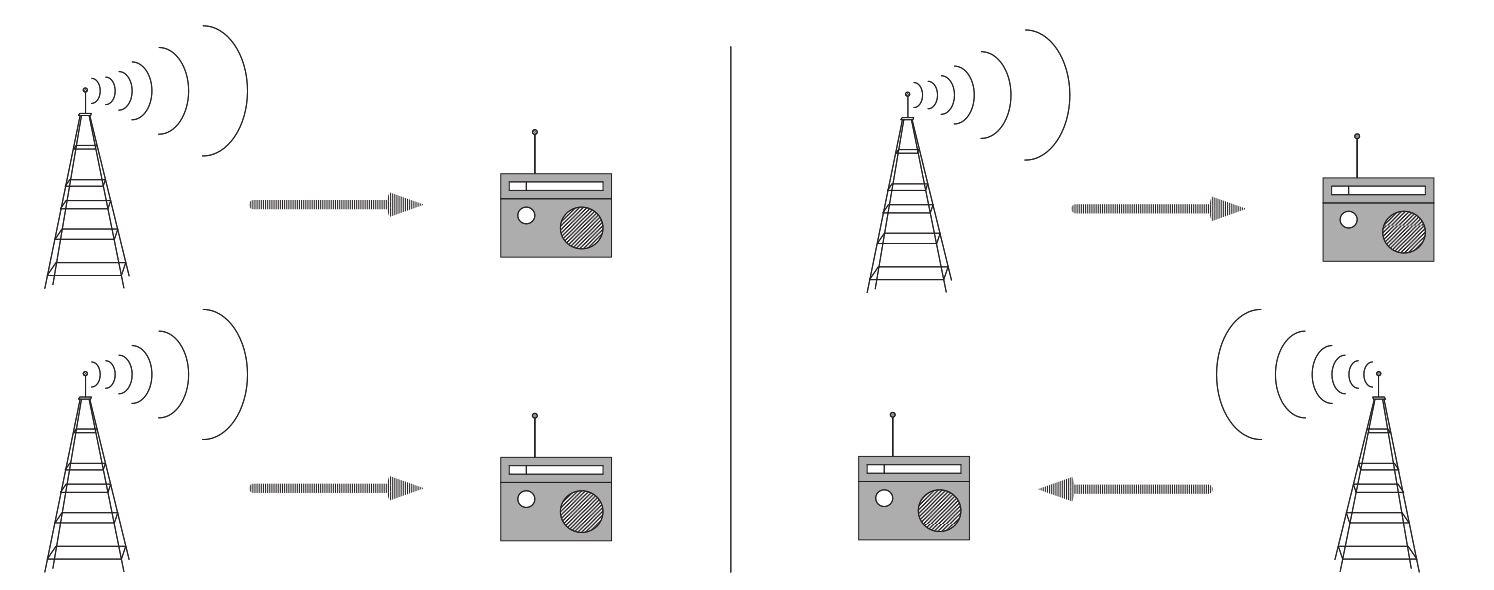
\includegraphics[width=\textwidth]{images/reversing.png} 
    \caption{Reversing one of the channel makes the channel have a non-zero capacity}
    \label{fig:reversing}
\end{figure}

Let's finally move to the respected old art and science of \textit{cryptography}. It's broadly described as the \textit{communication} between two parties \textit{who may not trust each other}. An important case for cryptography is when one party wants to send a secret message to another, without anyone eavesdropping. This is done through a \textit{cryptographic protocol}. Two main ways this can be done is through \begin{enumerate*}
    [label=(\alph*)] \item \textit{public key cryptosystems} \item \textit{private key ecosystems}
\end{enumerate*}.

In \textit{private key cryptosystems}, both party share a private key initially, using which they send \textit{encrypted} messages to each other. Hence only these two can \textit{decrypt} the message, no one else. But the main problem of this is, how are the private keys distributed? what if a third person eavesdrops while they're being distributed? He can get to know every secret message between them. An early discovery of QIC solves this, using \textit{quantum cryptography} or \textit{quantum key distribution}. The basic idea used from quantum mechanics is that if an eavesdropper tries to measure the private key when Alice and Bob are distributing it, they can see that the state of communication channel has changed. Hence they get to know someone's out there and restart it. 

In \textit{public key cryptosystems}, each party makes it's own 'public key', which is made \textit{available to the genreal public}. Using this key of Bob, Alice can encrypt the message. For a third person, it's \textit{extremely difficult} to decrypt this. Not even Alice can decrypt this in real time. Only Bob, who has the keys to his public key personally, can decrypt it. This is most popular these days. The encryption is done through \textit{RSA cryptosystem}. The key here is, it should be extremely decrypt the encryption only with the public key. For this, RSA uses something closely similar to factoring. But Shor's algorithm, run on a quantum computer can to this effectively. Few use discrete logarithm problem, which can also be done effectively by Shor's algorithm. This implies a need of quantum computing and quantum information.

The most striking of these in the study of \textit{quantum entanglement}. It is a unique quantum mechanical \textit{resource} which plays a key role in many applications of QIC. It's like iron to the classical world's bronze age. There's no proper theory of quantum entanglement as of now, a lot of effort is being made. Further study of quantum entanglement is going to lead to amazing new discoveries in quantum computation \subsection{Measurement in bases other than the computational basis}
If we try to represent the state of a system $\qv = \alpha \qo + \beta \qi$ in a different basis, $\ket{a}$ and $\ket{b}$, which are \textit{orthonormal}, we can write it as $\alpha'\ket{a}+\beta'\ket{b}$. According to the postulates of quantum mechanics, if we try to measure with respect to the basis $\ket{a}, \ket{b}$, we get \textit{a} with probability $|\alpha'|^2$ and \textit{b} with probability $|\beta'|^2$. We will learn more about the efficiency of measuring with respect to a basis in further study. of $\qo$ and $\qi$ as \begin{equation}
    \qv = \alpha \qo + \beta \qi,\ \alpha,\beta \in \mathbb{C}
\end{equation}
$\qo, \qi$ are known as \textit{computational basis states}. Unlike a classical bit, we can't determine state of a qubit. When we try observing/measuring it, we get $\qo$ with probability $|\alpha|^2$ and $\qi$ with probability $|\beta|^2$. Thus $|\alpha|^2 + |\beta|^2 = 1$. Hence we can think of the state as unit vector in a complex vector space with the computational bases. This unobservablity of a qubit makes up the heart of QIC. 

A state $\qv$ of a qubit can be represented as,
\begin{equation}
    \qv = e^{i\gamma}\left( \cos{\frac{\theta}{2}}\qo + e^{i\varphi}\sin{\frac{\theta}{2}}\qi  \right)
\end{equation}
which equal to this by a global factor $e^{i\gamma}$,
\begin{equation}
    \qv = \cos{\frac{\theta}{2}}\qo + e^{i\varphi}\sin{\frac{\theta}{2}}\qi
\end{equation}
$\theta, \varphi$ define a point on a sphere known as the \textit{Bloch sphere}; this thing describes many operations of qubits properly. But this doesn't generalize when it comes to multiple qubits.
\begin{figure}[H]
    \centering
    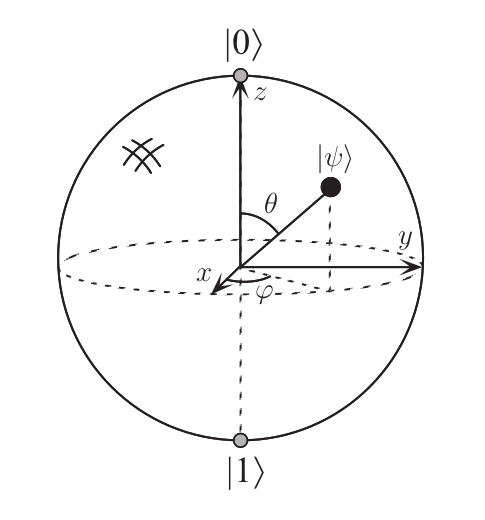
\includegraphics[width=0.5\textwidth]{images/bloch_sphere.png}
    \caption{Bloch sphere representation of a qubit.}
    \label{fig:bloch_sphere}
\end{figure}

\subsection{Multiple qubits}
State vector $\qv$ of a system of two qubits can be defined as,
\begin{equation}
    \qv = \alpha_{00} \ket{00}
         +\alpha_{01} \ket{01}
         +\alpha_{10} \ket{10}
         +\alpha_{11} \ket{11}
\end{equation}
It can be seen that it has four \textit{computational bases}, $\ket{00}, \ket{01}, \ket{10}, \ket{11}$. Even here when we measure the qubit, we get $x=(00, 01, 10, 11)$ with probability $|\alpha_x|^2$ and the qubit collapses to the state $\ket{x}$. By \textit{normalization}, $\sum_{x\in \{0,1\}^2} |\alpha_x^2| = 1$, where $\{ 0, 1\}^2$ is set of all strings with each character 0 or 1. For this set of two qubits, if we try to measure a subset of this, i.e a qubit, say first qubit, the probability of getting the output 0 is $|\alpha_{00}|^2+|\alpha_{01}|^2$ and after measuring, the system collapses to
\begin{equation}
    \ket{\psi'} =
    \frac{\alpha_{00} \ket{00}
         +\alpha_{01} \ket{01}}{\sqrt{|\alpha_{00}|^2+|\alpha_{01}|^2}}
\end{equation}
This is a similar collapse \textit{re-normalized} with a normalization constant.

Another interesting thing can be seen if we consider the Bell state,
\begin{equation}
    \qv = \frac{\ket{00}+\ket{11}}{2}
\end{equation}
If we try to measure $\qo$, we get the output 0 with probability $\frac{1}{2}$ and the bell state collapses to $\ket{00}$, and the output 1 with probability $\frac{1}{2}$ with the bell state collapsing to $\ket{11}$. We can see that if we get 0 we perfectly know about second qubit, i.e measurements are \textit{correlated}. Also, a set of $n$ systems can store $2^n$ amount of information, even though when we measure it, it collapses.

\section{Quantum Computation}
Similar to an electrical circuit, there's a \textit{quantum circuit} which performs operations on qubits using \textit{quantum gates}.
\subsection{Single qubit gates}
We can think of a \textbf{not} gate similar to it's classical analogue, which converts $\qo$ to $\qi$  and vice-versa. It's also linear, i.e \textbf{not} gate when acted on the state
\begin{equation}
    \alpha\qo + \beta\qi
\end{equation}
it interchanges $\qo$ and $\qi$ to give
\begin{equation}
    \alpha\qi + \beta\qo
\end{equation}
This fact is very important, which can be realised later. \textsc{not} gate can be represented by the matrix
\begin{equation}
    X \equiv \begin{bmatrix}
        0 & 1 \\ 1 & 0
    \end{bmatrix}
\end{equation}
For a matrix $U$ to be a \textit{quantum gate}, it has to be unitary and this is the \textit{only} constraint.

Few interesting gates are $Z$, which leaves $\qo$ unchanged while flips the sign of $\qi$,
\begin{equation}
    Z \equiv \begin{bmatrix}
        1 & 0 \\ 0 & -1
    \end{bmatrix}
\end{equation}
The output is equal upto a relative phase factor, the other is the \textit{Hadamard gate}, H given by
\begin{equation}
    H \equiv \frac{1}{\sqrt{2}}\begin{bmatrix}
        1 & 1 \\ 1 & -1
    \end{bmatrix}
\end{equation}
\begin{figure}[H]
    \centering
    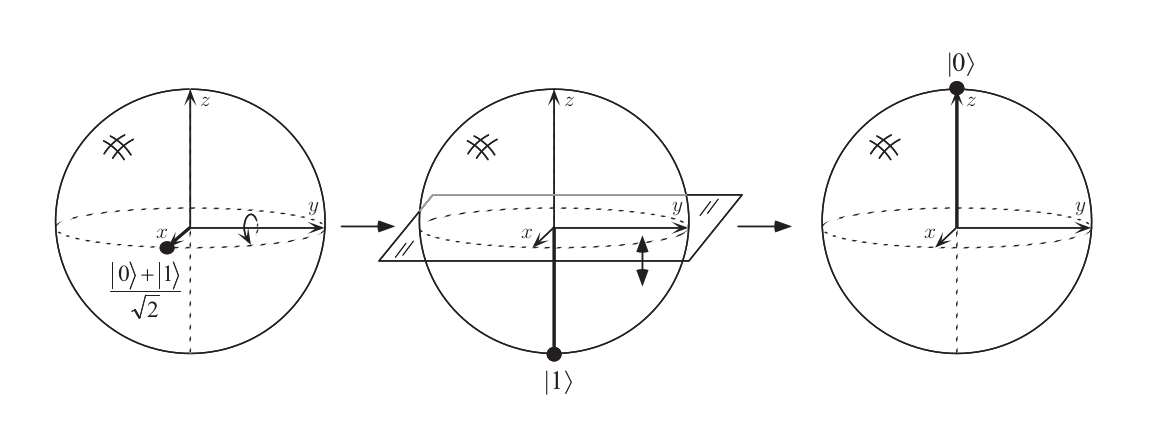
\includegraphics[width=\textwidth]{images/hadmard_bloch.png}
    \caption{Hadmard gate acting on $\frac{\qo + \qi}{\sqrt{2}}$ to give $\qo$}
    \label{fig:hadmard_bloch}
\end{figure}
This get takes $\qo$ to $\frac{\qo + \qi}{\sqrt{2}}$ and $\qi$ to $\frac{\qo-\qi}{2}$. In the Bloch sphere point of view, this rotates the sphere first w.r.t $\hat{y}$ axis by $90^\circ$ and then rotates w.r.t $\hat{x}$ axis by $180^\circ$.

These qubit gates are summarised as
\begin{figure}[H]
    \centering
    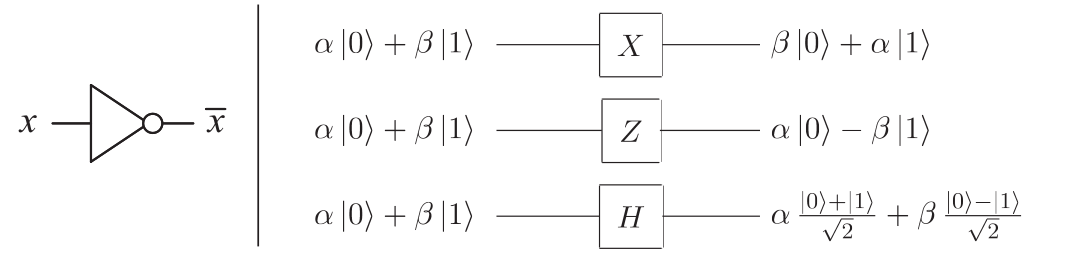
\includegraphics[width=\textwidth]{images/qubit_gates.png}
    \caption{Single bit (left) and Qubit (right) logic gates.}
    \label{fig:qubit_gates}
\end{figure}
We can see that any unitary matrix corresponds to a single qubit gate. Since, there are infinitely many unitary matrices, there are infinitely many single qubit gates. But we can represent this set only with a few single qubit gates. It can be shown that any unitary matrix  $U$ can be written as
\begin{equation}
    U = e^{i\alpha}\begin{bmatrix}
        e^{-i\beta/2} & 0 \\ 0 & e^{i\beta/2}
    \end{bmatrix}
    \begin{bmatrix}
        \cos{\frac{\gamma}{2}} & \sin{\frac{\gamma}{2}} \\ \sin{\frac{\gamma}{2}} & -\cos{\frac{\gamma}{2}}
    \end{bmatrix}
    \begin{bmatrix}
        e^{-i\delta/2} & 0 \\ 0 & e^{i\delta/2}
    \end{bmatrix}
\end{equation}
This can be seen as a rotation about $\hat{z}$ axis then a rotation about $\hat{y}$ axis followed by a rotation about $\hat{z}$ axis again and global phase shift. Any single qubit gate can be decomposed into a form like this. Also, any computation on a \textit{finite} number of qubits can be generated by a \textit{finite} set of gates known as the \textit{universal} for quantum computation.

\subsection{Multiple qubit gates}
For classical bits, there are \textsc{and, or, nand, nor, xor} gates. \textsc{nand} gate is considered as the \textit{universal gate} as any function of bits can be constructed using \textsc{nand} gates. \textsc{xor} gate can't do this. There's a special multi-qubit quantum gate, known as \textit{controlled-}\textsc{not} gate or \textsc{cnot} gate, which has a \textit{control qubit} and a \textit{target qubit}. If the control qubit is 0, nothing happens to target qubit, whereas if it's 1, the target qubit is flipped. i.e,
\begin{equation}
    \ket{00} \xrightarrow{} \ket{00}; \ket{01} \xrightarrow{} \ket{01};
    \ket{10} \xrightarrow{} \ket{11}; \ket{11} \xrightarrow{} \ket{10}
\end{equation}
The \textsc{cnot} gate is similar to the \textsc{xor} gate, because it's just doing $\ket{A, B} \xrightarrow[]{} \ket{A, B\oplus A}$, where $B\oplus A$ is just the \textsc{xor} gate, is the sum modulo two. There are no similar generalisations for classical \textsc{xor, nand} because they're \textit{irreversible} or \textit{non-invertible}. Information is lost upon the action of these gates which is irretrievable. \textsc{cnot} and single qubit gates are prototypes for all other gates because of the following \textit{universality} result: \textit{Any multiple qubit gate may be composed from \textsc{cnot} and single qubit gates.} 
\begin{figure}[H]
    \centering
    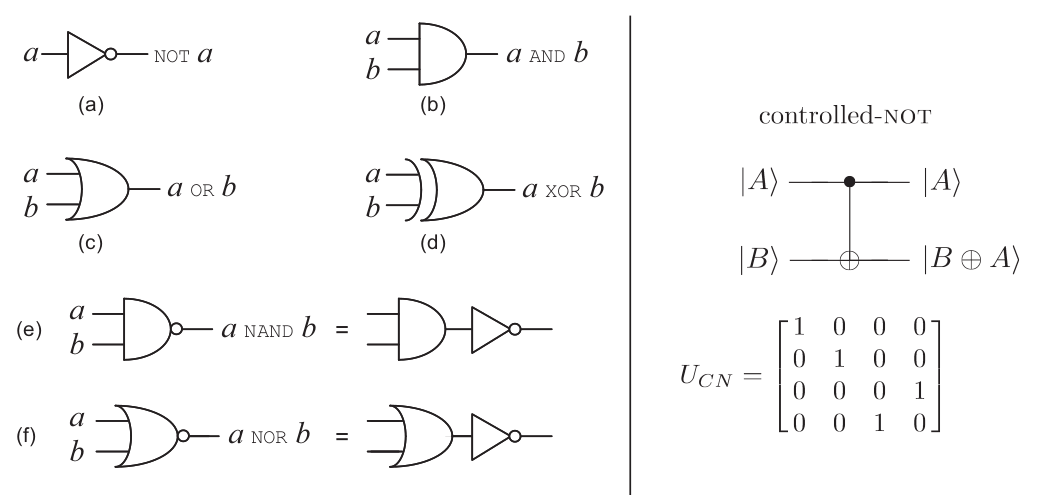
\includegraphics[width=\textwidth]{images/multi_gates.png}
    \caption{Figure on left shows common bit gates; The right figure shows the \textsc{cnot} gate along with it's matrix representation, in the order of $\ket{00}, \ket{01}, \ket{10}$ and $\ket{11}$.}
    \label{fig:enter-label}
\end{figure}

\subsection{Measurement in bases other than the computational basis}
If we try to represent state of a system $\qv = \alpha \qo + \beta \qi$ in a different bases, $\ket{a}$ and $\ket{b}$ which are \textit{orthonormal}as $\alpha'\ket{a}+\beta'\ket{b}$. By postulates of quantum mechanics, if we try to measure w.r.t basis $\ket{a}, \ket{b}$ we get \textit{a} with probability $|\alpha'|^2$ and \textit{b} with probability $|\beta'|^2$. We'll learn more about how efficient is it to measure w.r.t a basis in further study.

\subsection{Quantum circuits}
Similar to classical circuits, quantum circuits are made of wires, which don't necessarily represent physical wires, rather the passage of time or a physical photon moving in space. Let's first look at an example.
\begin{figure}[H]
    \centering
    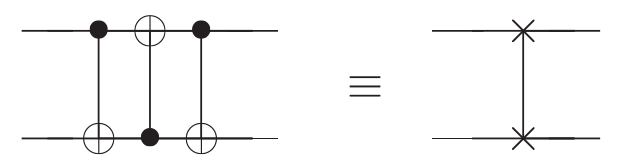
\includegraphics[width=0.5\textwidth]{images/simple_circuit.png}
    \caption{Circuit which swaps two qubits and an equivalent circuit since this is more useful and commonly used.}
    \label{fig:simple-circuit}
\end{figure}
The above circuit swaps two qubits, which can be seen this way considering two qubits with states $\ket{a}$ and $\ket{b}$ as input,
\begin{align}
    \ket{a,b} &\xrightarrow{} \ket{a, b\oplus a} \\
              &\xrightarrow{} \ket{a \oplus (b \oplus a), b \oplus a} = \ket{b, b\oplus a}\\
              &\xrightarrow{} \ket{b, (b\oplus a) \oplus b} = \ket{b, a}
\end{align}
There are few features in classical circuits which aren't seen in quantum circuits. First one is \textit{loops} are not allowed, i.e the circuit is \textit{acyclic}. Second, classical circuit allows joining of wires, an operation known as \textsc{fanin}. Here, the bitwise \textsc{or} operator of inputs is taken. However, information is lost and thus this is irreversible, thus not being allowed in quantum circuits. Thirdly, the inverse of this, where multiple copies of a single bit is made in a classical circuits, known as \textsc{fanout} is not allowed in quantum circuits. We can show that it's impossible to copy a qubit.

There's another important gate, which is in some sense generalisation of \textsc{cnot} gate, \textit{controlled-U} gate. which is represented by this
\begin{figure}[H]
    \centering
    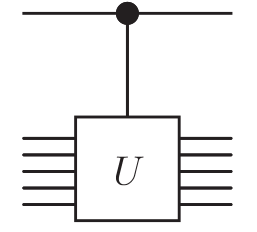
\includegraphics[width=0.2\textwidth]{images/controlled_u.png}
    \caption{Controlled-U gate}
    \label{fig:controlled-u}
\end{figure}
This has similar logic, it's associated with a \textit{unitary matrix} U and takes 1 qubit as the \textit{control qubit}, and $n$ qubits as \textit{target qubits} as inputs. If the control qubit is set to 0, then nothing happens to target qubits. If control qubit is set to 1, then the gate $U$ is applied to all the target qubits. In this sense, \textsc{cnot} gate is the special case when $n=1$ and $U=X$, as shown
\begin{figure}[H]
    \centering
    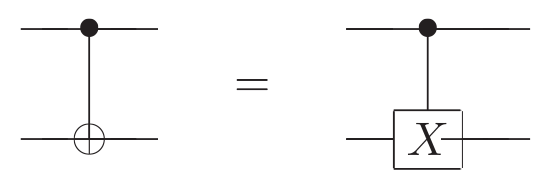
\includegraphics[width=0.5\textwidth]{images/cnot_as_cu.png}
    \caption{Two different representations of \textsc{cnot} gate.}
    \label{fig:cnot-as-cu}
\end{figure}

There's another important operation, known as measurement shown by the 'meter' symbol.
\begin{figure}[H]
    \centering
    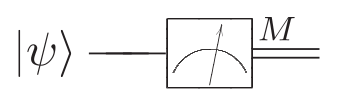
\includegraphics[width=0.4\textwidth]{images/measurement.png}
    \caption{Quantum circuit symbol for measurement.}
    \label{fig:measurement}
\end{figure}
As expected, this outputs a probabillistic classical bit M (which is 0 with probability $|\alpha|^2$ or 1 with probability $|\beta|^2$) if a qubit with state $\qv = \alpha\qo + \beta\qi$ is given as input. Thus, the output is distinguished from a qubit by drawing a double-line wire.

\subsection{Qubit copying circuit?}
First we'll look at a classical example, suppose we have a bit $x$ which we want to copy, we'll use a \textsc{cnot} gate with $x$ and a 'scratchpad bit' 0 as first and second inputs respectively, it'll copy x succesfully as shown
\begin{figure}[H]
    \centering
    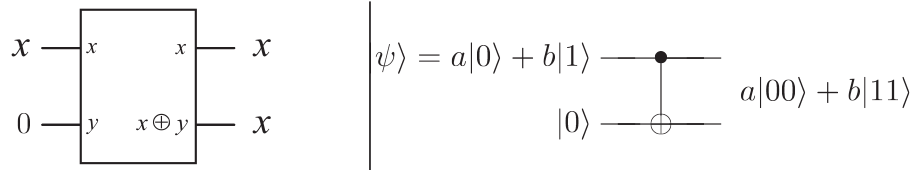
\includegraphics[width=0.8\textwidth]{images/qubit_copy.png}
    \caption{Trying to copy a classical bit (left) and a qubit (right)}
    \label{fig:qubit-copy}
\end{figure}
But if we try copying a qubit with state $\qv = a\qo + b\qi$ in a similar manner using a \textsc{cnot} gate, we can give $\qo$ as an input along with it as
\begin{equation}
    \left[ a\qo + b\qi \right]\qo = a\ket{00} + b\ket{10}
\end{equation}
applying the \textsc{cnot} gate gives $a\ket{00} + b\ket{11}$ as the output. We'd expect the output $\qv\qv$ if we copied $\qv$ succesfully. But that would mean the output should be
\begin{equation}
    \qv\qv = a^2\ket{00} + ab\ket{01} + ab\ket{10} + b^2\ket{11}
\end{equation}
But as we've seen above, it's only possible when $ab = 0$, i.e $a=0$ or $b=0$ i.e we want to copy either $\qo$ or $\qi$. Hence we can't copy $\qv$. It can be shown in general that it is impossible to copy a general qubit with unkown quantum state, if we construct a cloning gate, it can copy different state qubits $\ket{a}$ and $\ket{b}$ only if they are orthogonal. This is known as the \textit{no-cloning} theorem.

There's another way to look at it. An unkown qubit contains some 'hidden' information that isn't directly accessible with a measurement. What's happening above is we get $a\ket{00} + b\ket{11}$, which if we measure we obtain either 0 or 1 using which the other qubit is completely determined. Thus, no extra information is gained. But if we were able to copy $\qv$, then the other qubit contains some more information, contradicting our knowledge, thus a copy can't be created.

\subsection{Example: Bell states}
Let's take a look at a circuit which has a Hadamard gate on first input followed by a \textsc{cnot} gate, as shown
\begin{figure}[H]
    \centering
    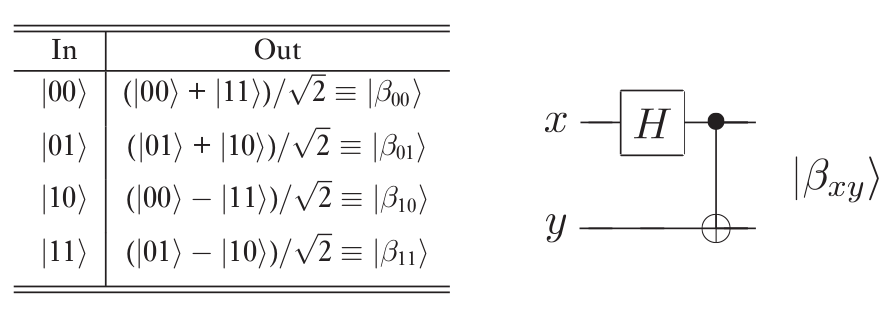
\includegraphics[width=0.9\textwidth]{images/bell_circuit.png}
    \caption{Quantum circuit which creates Bell states, along with it's quantum `truth table'}
    \label{fig:bell-circuit}
\end{figure}
As shown in the truth table, the Hadmard gate first transforms  the first qubit into a superposition after which the \textsc{cnot} gate inverts the target only when control is 1. The output states are
\begin{align}
    \ket{\beta_{00}} &= \frac{\ket{00}+\ket{11}}{\sqrt{2}} \\
    \ket{\beta_{01}} &= \frac{\ket{01}+\ket{10}}{\sqrt{2}} \\
    \ket{\beta_{10}} &= \frac{\ket{00}-\ket{11}}{\sqrt{2}} \\
    \ket{\beta_{11}} &= \frac{\ket{01}-\ket{10}}{\sqrt{2}} 
\end{align}
These are known as the \textit{Bell states} or \textit{EPR states} or \textit{EPR pairs} as their strange properties were found by Einstein, Podolsky and Rosen. Generalizing it,
\begin{equation}
    \ket{\beta_{xy}} = \frac{\ket{0y}+(-1)^x\ket{1\bar{y}}}{\sqrt{2}}
\end{equation}
where $\bar{y}$ is the negation of $y$, $\ket{\beta_{xy}}$ denotes the output when the input given is $\ket{xy}$.

\subsection{Example: quantum teleportation}
It's a non-trivial, surprising and a fun thing! Quantum teleportation is a technique using which we can move quantum states around even in the absence of a quantum communication channel. Consider Alice and Bob, who've met long ago and have shared an EPR pair. Now Alice has a new qubit in state $\qv$ which she doesn't know and has to deliver to Bob. She can only send \textit{classical} information. 

Intuitively, it's pretty bad situation. It's not possible for her to get to know the state $\qv$ completely as she only has one copy of the qubit. Also if she knew the state, it's impossible to transfer this information to Bob, as $\qv$ takes values in \textit{continuous} space, hence requiring infinite amount of time. Quantum teleportation provides a way for it. 

In short, what happens is she measures this state $\qv$ along with the half of her EPR pair. She gets a result in 00, 01, 10 or 11 which she then sends to Bob. Using this information Bob can perform some operations and completely retrieve the state $\qv$ without even getting to know it. Shown using a quantum circuit
\begin{figure}[H]
    \centering
    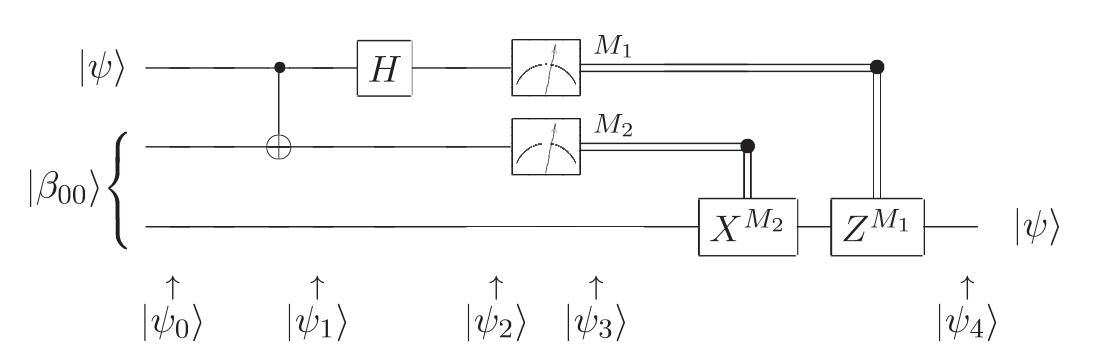
\includegraphics[width=0.8\textwidth]{images/teleportation.png}
    \caption{Quantum circuit showing the teleportation process}
    \label{fig:teleportation}
\end{figure}
Suppose Alice and Bob are sharing $\ket{\beta_{00}}$ and the $\qv$, assuming second input is from alice, overall input to the circuit is 
\begin{align}
    \ket{\psi_0} &= \qv\ket{\beta_{00}} \\
    &= (\alpha\qo + \beta\qi)\left(\frac{\ket{00} + \ket{11}}{\sqrt{2}}\right)\\
    &= \frac{1}{\sqrt{2}}\left[ \alpha\qo\ket{00} + \alpha\qo\ket{11} + \beta\qi\ket{00} + \beta\qi\ket{11} \right]
\end{align}
which when sent through \textsc{cnot} gate on first two qubits gives $\ket{\psi_1}$
\begin{align}
    \ket{\psi_1} &= \frac{1}{\sqrt{2}}\left[ \alpha\qo(\ket{00}+\ket{11}) + \beta\ket{1}(\ket{10}+\ket{01}) \right]
\end{align}
The first qubit is then sent through Hadamard gate, which upon simplifying gives
\begin{align}
    \ket{\psi_2} &= \frac{1}{2}\left[ \alpha(\qo+\qi)(\ket{00}+\ket{11}) + \beta(\qo-\qi)(\ket{10}+\ket{01}) \right]
\end{align}
Now Alice measures the first two qubits of this whole system, giving outputs as $M_1$ and $M_2$ respectively. Based on  what is measured as $M_1M_2$ we can know what is the final state of the qubit Bob has, which is
\begin{align}
    00 &\longmapsto \ket{\psi_3(00)} \equiv \left[ \alpha\qo + \beta\qi \right] \\
    01 &\longmapsto \ket{\psi_3(01)} \equiv \left[ \alpha\qi + \beta\qo \right] \\
    10 &\longmapsto \ket{\psi_3(10)} \equiv \left[ \alpha\qo - \beta\qi \right] \\
    11 &\longmapsto \ket{\psi_3(11)} \equiv \left[ \alpha\qi - \beta\qo \right] 
\end{align}
Now Alice sends these two classical bits to Bob, according to which he knows what kind of transformation to apply on his qubit to transform it to the qubit Alice had. We can verify that he has to apply the matrix $Z^{M_1}X^{M_2}$ to get $\ket{\psi_4}$ i.e $\qv$. Note that the order of matrix multiplication is opposite to the time flow as shown in the circuit diagram.

As we had to transfer classical bits, which can't be done faster than the speed of light, quantum teleportation also can't be done faster than light and is limited by the speed of transfer of the classical bits as faster than light travel could possibly result in sending information backwards in time.

Also note that we haven't created a copy of $\qv$ which would contradict our \textit{no-cloning theorem}. It's because the origin qubit we had in state $\qv$ changes into the state $\qo$ or $\qi$ depending on the value of $M_1$ at the end of the process. Quantum teleportation shows that two classical bits can become a resource at least equal to one qubit information.

\section{Quantum Algorithms}
We'll explore what kind of problems a quantum computer can solve better than a classical computer. How a quantum computer can solve classical problems, we'll also look through well known quantum algorithms.

\subsection{Classical algorithms on a quantum computer}
It turns out that we can simulate any classical circuit using a quantum circuit. It should be possible as physicists believe that everything is explainable using quantum mechanics. We'll kind of prove it in the further discussion. Also, the reason we don't directly use quantum gates to simulate classical gates is that quantum gates are inherently \textit{reversible}, whereas many classical gates such as \textsc{nand} gates are inherently irreversible.

Any classical circuit can be replaced by a reversible elements known as the \textit{Toffoli gate}. Toffoli gate is a reversible gate which takes in three input bits $a,b,c$. If we both the first two input  bits (\textit{control} bits) $a,b$ are 1, it flips the third bit (\textit{target} bit) else it doesn't affect it. It's equivalent to $(a,b,c)\longrightarrow(a,b,c\oplus ab)$ and is represented by this
\begin{figure}[H]
    \centering
    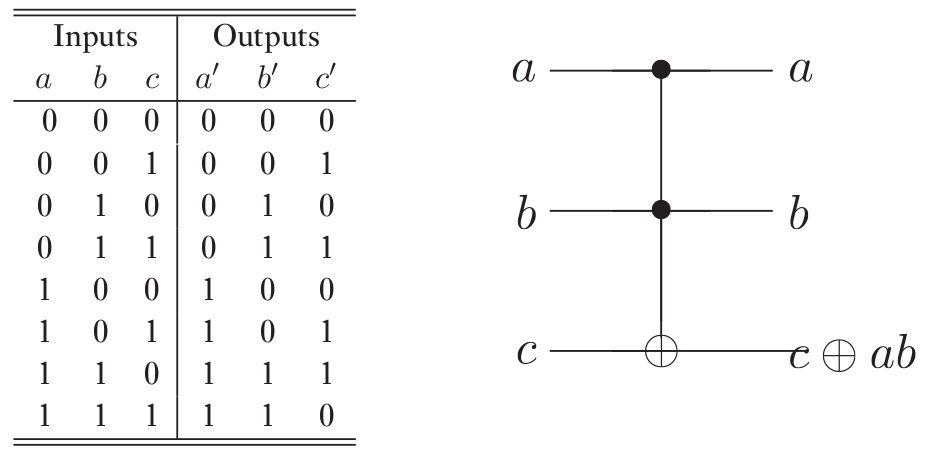
\includegraphics[width=0.7\textwidth]{images/toffoli.png}
    \caption{Left: Truth table for the Toffoli gate, Right: circuit representation of the Toffoli gate.}
    \label{fig:toffoli}
\end{figure}
\begin{figure}[H]
    \centering
    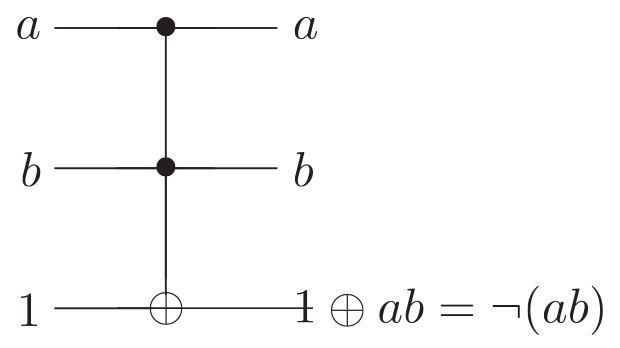
\includegraphics[width=0.4\textwidth]{images/toffoli_nand.png}
    \caption{\textsc{nand} gate simulated using toffoli gate.}
    \label{fig:toffoli-nand}
\end{figure}
\begin{figure}[H]
    \centering
    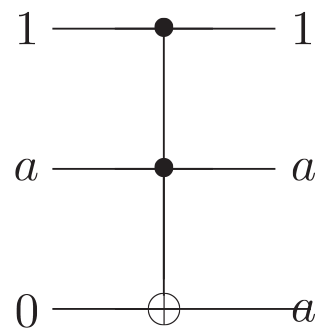
\includegraphics[width=0.2\textwidth]{images/toffoli_fanout.png}
    \caption{\textsc{fanout} gate simulated using Toffoli gate}
    \label{fig:toffoli-gate}
\end{figure}
Toffoli gate can also simulate \textsc{nand} and \textsc{fanout} gates as shown above. Even though we've shown the classical implementation of toffoli gate above, it can be implemented as a quantum logic gate. It works in a similar way as the classical toffoli gate. For example flipping third qubit of $\ket{110}$ to give $\ket{111}$. It can also be proved that this is a valid unitary quantum gate by constructing the corresponding 8 by 8 matrix, $U$. Thus, the quantum toffoli gate can simulate irreversible classical gates, ensuring that quantum computers are capable of what classical computers can do. Not only a classical computer, a quantum computer can simulate a non-deterministic computer, i.e which can generate random bits. A simple way it can do it is preparing a state $\qo$ then applying the Hadamard gate to it, giving $\frac{\qo+\qi}{\sqrt{2}}$ which upon measuring gives $\qo$ or $\qi$ with 50\% probability, thus generating a random number and efficiently simulating a non-deterministic classical computer. A quantum computer is way more advantageous than this and can perform much more powerful functions as we'll discuss further.

\subsection{Quantum parallelism}
\textit{Quantum parallelism} is a fundamental feature of quantum computers. They can evaluate a function $f(x)$ \textit{simultaneously} at many different values. 

Suppose $f:\{0,1\}\xrightarrow{}\{0,1\}$ be a function with a one-bit domain and range. A way of computing this function using a quantum computer is to generate a transform using quantum logic gates which transforms a given state $\ket{x,y} \longrightarrow \ket{x, y\oplus f(x)}$. When $y=0$ the state of the second qubit is just $f(x)$. We name this map as $U_f$ as shown
\begin{figure}[H]
    \centering
    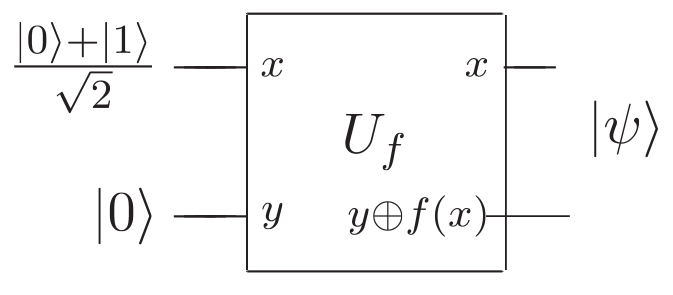
\includegraphics[width=0.6\textwidth]{images/parallelism.png}
    \caption{Quantum circuit for calculating $f(0)$ and $f(1)$ simultaneously. $U_f$ is a quantum circuit which takes $\ket{x,y}$ to $\ket{x, y\oplus f(x)}$}
    \label{fig:parallelism}
\end{figure}
Now if we want to compute both $f(0)$ and $f(1)$ simultaneously, we'll use the superposition state $\frac{\qo + \qi}{\sqrt{2}}$, which can be generated from $\qo$ using a Hadmard gate, and apply $U_f$ on it. We then get
\begin{equation}
    \frac{\ket{0, f(0)}+\ket{1, f(1)}}{\sqrt{2}}
\end{equation}
which contains information about both $f(1)$ and $f(2)$. Thus we've in some sense evaluated both $f(0)$ and $f(1)$ parallely using a single circuit. In classical parallelism, we would have had to construct multiple circuits to evaluate the function at multiple points parallely. We can generalize it to a function which take \textit{multiple} bits as inputs. First we'll apply \textit{Hardmard transform} sometimes known as \textit{Welsh-Hadmard transform} parallely on $n$ qubits. Circuit for $n=2$ is as shown
\begin{figure}[H]
    \centering
    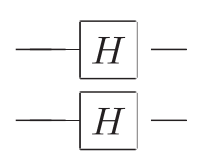
\includegraphics[width=0.3\textwidth]{images/parallel_hadmard.png}
    \caption{Two Hadmard gates ($H^{\otimes 2}$) acting on two qubits parallely.}
    \label{fig:parallel-hadmard}
\end{figure}
For $n=2$ we get
\begin{align}
    \left( \frac{\qo + \qi}{\sqrt{2}} \right) \left( \frac{\qo + \qi}{\sqrt{2}} \right)
    &= \frac{\ket{00}+\ket{01}+\ket{10}+\ket{11}}{2}
\end{align}
This operation can be represented by $H^{\otimes 2}$. For $n$ qubits, as $H^{\otimes n}$. Performing Hadmard transform on $n$ qubits all initialised to $\qo$ gives
\begin{equation}
    \frac{1}{\sqrt{2^n}}\sum_x \ket{x}
    \label{hadmard-eqn-n-qubits}
\end{equation}
Where $x$ is all the possible combinations of $n$ 0's and 1's. 

Now if we want to use quantum parallelism to compute $f(x)$ which takes multi-bit values at multiple values, we first prepare a quantum system of $n+1$ qubits with state $\qo^{\otimes n}\qo$ which upon applying Hadmard transform on first $n$ qubits gives \ref{hadmard-eqn-n-qubits}. This followed by $U_f$ produces
\begin{equation}
    \frac{1}{\sqrt{2^n}}\sum_x \ket{x}\ket{f(x)}
\end{equation}
Do note that we can still \textit{measure} the value of f(x) only at one input. For quantum parallelism to be useful, we need some method to \textit{extract} more informatioin from superposition states like $\sum_x\ket{x}\ket{f(x)}$ .

\subsection{Deutsch's algorithm}
Using this, we can get `global information' about $f(x)$. It combines quantum parallelism with another quantum property known as \textit{interference}. To see how this works, let's create our first qubit as superposition $\frac{\qo + \qi}{\sqrt{2}}$ using Hadmard gate on $\qo$ and our second qubit as superposition $\frac{\qo-\qi}{\sqrt{2}}$ using Hadmard gate on $\qi$. Now let's use this circuit
\begin{figure}[H]
    \centering
    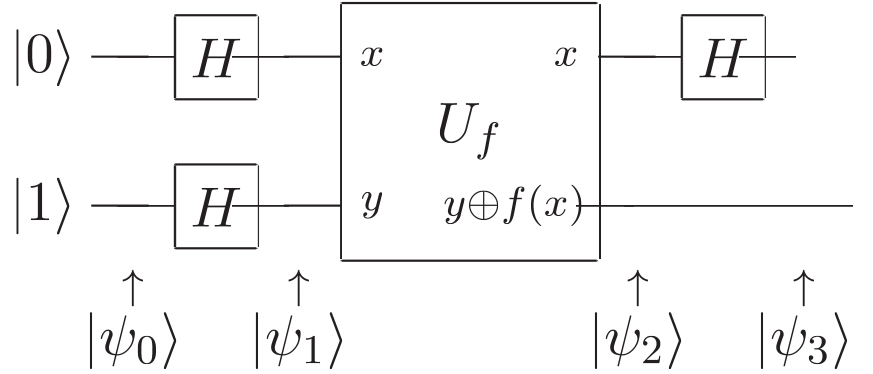
\includegraphics[width=0.7\textwidth]{images/deutsch_algo.png}
    \caption{Quantum circuit implementing Deutsch's algorithm}
    \label{fig:deutsch-algo}
\end{figure}
Our input to this will be
\begin{equation}
    \ket{\psi_0} = \qo\qi
\end{equation}
When Hadmard gates are acted upon them, they become
\begin{equation}
    \ket{\psi_1} = \begin{bmatrix}
        \frac{\qo+\qi}{\sqrt{2}}
    \end{bmatrix}\begin{bmatrix}
        \frac{\qo-\qi}{\sqrt{2}}
    \end{bmatrix}
    \label{eq:U_f_deutsch}
\end{equation}
With a little thought, it can be seen that applying $U_f$ on $\ket{x}(\qo-\qi)/\sqrt{2}$ gives $(-1)^{f(x)}\ket{x}(\qo-\qi)/\sqrt{2}$, Hence applying $U_f$ to $\ket{\psi_1}$ gives
\begin{equation}
    \ket{\psi_2} = \begin{cases}
        \pm\left[
            \frac{\qo+\qi}{\sqrt{2}}
        \right]
        \left[
                \frac{\qo-\qi}{\sqrt{2}}
        \right] &\text{if } f(0) = f(1) \\\\
        \pm\left[
            \frac{\qo-\qi}{\sqrt{2}}
        \right]
        \left[
            \frac{\qo-\qi}{\sqrt{2}}
        \right]&\text{if } f(0) \neq f(1)
    \end{cases}
\end{equation}
Applying the final Hadamard gate on this give $\ket{\psi_3}$
\begin{equation}
    \ket{\psi_3} = \begin{cases}
        \pm \qo \left[ \frac{\qo-\qi}{\sqrt{2}} \right]
        &\text{if } f(0) = f(1)\\
        \pm \qi \left[ \frac{\qo-\qi}{\sqrt{2}} \right]
        &\text{if } f(0) \neq f(1)
    \end{cases}
\end{equation}
This can be condensed more by observing that $f(0)=f(1) \implies 0 = f(0)\oplus f(1)$ and $f(0) \neq f(1) \implies 1 = f(0)\oplus f(1)$, Thus
\begin{equation}
    \ket{\psi_3} = \pm \ket{f(0) \oplus f(1)} \left[ \frac{\qo-\qi}{\sqrt{2}} \right]
\end{equation}
Thus, we can measure $f(0)\oplus f(1)$ by measuring the first qubit. This is really interesting since we found out $f(0)\oplus f(1)$ which is a \textit{global} property of $f(x)$ by just evaluating $f(x)$ \textit{once}! Thus distinguishes a quantum parallelism from even a classical computer. Even a probabilistic classical computer could determine $f(0)$ or $f(1)$ with probability $\frac{1}{2}$ each, a quantum computer evaluates both at once. We can get global information about function by cleverly chosing operation and gates so that the two evaluations \textit{interfere} with each other to give us information like this, which is not possible in classical computers.

\subsection{The Deutsch-Jozsa algorithm}
This is a generalisation to the Deutsch's algorithm. It's application, known as \textit{Deutsch's problem} is described as following. Suppose Alice and Bob are far apart, Alice is in Amsterdam and Bob is in Boston. Alice sends a number $x$ out of $\{ 0,\cdots,2^n-1 \}$ through a letter to Bob. Bob computes a function $f(x)$ which yields the result of either 0 or 1 and mails it back to Alice. Alice needs to find out whether the function $f(x)$ is \textit{constant} or \textit{balanced} i.e 0 for half the values and 1 for the other half by sending as many mails as she can. Using classical means we can figure out that she would need $2^{n-1}+1$ mails to be sent in the worst case.

We can offer a much better solution using qubits if we're sure that Bob is willing to calculate $f(x)$ using a unitary transform $U_f$ in a single interaction. To see how this works, Alice has a set of $n$ qubits each prepared as $\qo$ in which she stores the query $(\sim x)$ and another qubit prepered as $\qi$ where she stores the answer $(\sim f(x))$. She then applies Hadmard transform on all $n+1$ qubits after which she sends these to Bob. Bobs first applies $U_f$ on them and then Alice applies Hadmard transform on the first n qubits such that she gets information about $f(x)$ and thus the solution. We'll look through how this happens. Take a look at the circuit
\begin{figure}[H]
    \centering
    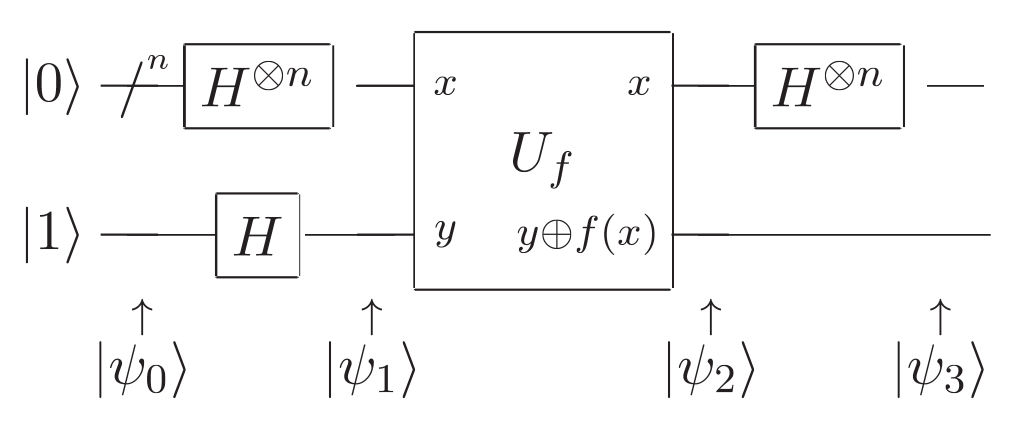
\includegraphics[width=0.7\textwidth]{images/deutsch_jozsa.png}
    \caption{Implementation of Deutsch-Jozsa algorithm, the cross represents $n$ qubits}
    \label{fig:deutsch-jozsa}
\end{figure}
So the input state is
\begin{equation}
    \ket{\psi_0} = \qo^{\otimes n}\qi
\end{equation}
When the Hadmard transform is applied, the query qubits turn into a superposition of $\ket{x}$ where $x$ is binary representation of all numbers in $\{ 0, \cdots, 2^n -1 \}$ 
\begin{equation}
    \ket{\psi_1} = \sum_{x} \frac{\ket{x}}{\sqrt{2^n}} \left[ \frac{\qo-\qi}{\sqrt{2}} \right]
\end{equation}
This is sent to Bob, he applies $U_f$ to $\ket{\psi_1}$ which results in $\ket{\psi_2}$ using similar result as in \ref{eq:U_f_deutsch}
\begin{equation}
    \ket{\psi_2} = \sum_x \frac{\ket{x}}{\sqrt{2^n}}(-1)^{f(x)}\left[ \frac{\qo-\qi}{\sqrt{2}}\right]
\end{equation}
Now comes the tricky part when Alice applies Hadmard gate on first $n$ qubits. Let's just see what happens when Hadamard transform is applied to $\ket{x}$ which is just a binary string (representation of some number $\in \{0,\cdots,2^n-1\}$). We get another superposition of all possible basis states $\ket{z}$ whose quotients are $(-1)^{xz}$ which is bitwise multiplication/\textsc{and} of $x$ and $z$ along with the normalization constant.
\begin{equation}
    H\ket{x} = \sum_z \frac{(-1)^{xz}\ket{z}}{\sqrt{2^n}}
\end{equation}
Thus the final output Alice gets is
\begin{equation}
    \ket{\psi_3} = \sum_x \sum_z \frac{(-1)^{xz+f(x)}\ket{z}}{2^n}\left[ \frac{\qo-\qi}{\sqrt{2}} \right]
\end{equation}
Looking at first n qubits, coefficient of $\qo^{\otimes n}$ turnes out to be just $\sum_x \frac{(-1)^{f(x)}}{2^n}$. Now note that if $f(x)$ was constant $\sum_x(-1)^{f(x)}$ would be $\pm 2^n$, which would mean coefficient of $\qo^{\otimes n}$ is $\pm1$. Since norm of state of a system should be 1 coefficients of all other $\ket{z}$ would be 0. Thus, Alice would only measure $\qo^{\otimes n}$. Now in the case when $f(x)$ is balanced, coefficient of $\qo^{\otimes n}$ would be 0. Hence, Alice would never get the measurement result as 0.
\begin{center}
    \textit{
    Alice gets $\qo^{\otimes n}$ upon measuring $\ket{\psi_3} \iff f(x)$ is constant
    }
\end{center}
Thus by measuring the query register Alice can get to know the answer in just one correspondence. Let's summarise this algorithm

\begin{algorithm}[H]
    \SetAlgoLined\DontPrintSemicolon
    \caption{Deutsch-Jozsa}
    \SetKwInOut{KwIn}{Inputs}
    \SetKwInOut{KwOut}{Outputs}
    \SetKwInOut{KwRun}{Runtime}
    \SetKwProg{myprog}{Procedure}{}{}

    \KwIn{A black box $U_f$ which performs the transformation $\ket{x}\ket{y} \longrightarrow \ket{x}\ket{y\oplus f(x)}$, $x \in \{0,\cdots,2^n-1\}$ and $f(x) \in \{0,1\}$. It's guaranteed that $f(X)$ is either \textit{balanced} or \textit{constant}.}
    \KwOut{0 if and only if $f$ is constant.}
    \KwRun{One evaluation of $U_f$, always succeeds.}
    \myprog{}{
    $\qo^{\otimes n}\qi$ \tcp*{initialize state}\;
    $\longrightarrow \frac{1}{\sqrt{2^n}}\sum_{x=0}^{2^n-1}\ket{x}\left[ \frac{\qo-\qi}{\sqrt{2}} \right]$ \tcp*{create superposition using Hadmard gates}\;
    $\longrightarrow \sum_x (-1)^{f(x)}\ket{x}\left[ \frac{\qo-\qi}{\sqrt{2}} \right]$ \tcp*{calculate $f$ using $U_f$}\;
    $\longrightarrow\sum_z \sum_x \frac{(-1)^{xz+f(x)}\ket{z}}{2^n}\left[ \frac{\qo-\qi}{\sqrt{2}} \right]$ \tcp*{perform Hadmard transform}\;
    $\longrightarrow z$ \tcp*{measure to obtain output}
    }{}
\end{algorithm}

This is a seed for quantum algorithms. But it has it's own problems, such it has no real world application. It can be solved in a more realistic manner using a probabilistic computer.

\subsection{Quantum algorithms summarized}
Broadly speaking, quantum computers are good at solving three classes of problems. First one based upon quantum versions of Fourier transform, Deutsch-Jozsa algorithm, Shor's algorithm and discrete logarithm come under this class. Second class is quantum search algorithms. Third class of algorithms is quantum simulation, using which a quantum computer can simulate a quantum system. Let's look at each of these
\subsubsection{Quantum algorithms based on Fourier transform}
The discrete Fourier transform is described as transforming the set $x_0, \cdots, x_{N-1}$ of N complex numbers into the set of complex numbers $y_1,\cdots,y_{N-1}$ according to this
\begin{equation}
    y_k \equiv \frac{1}{\sqrt{N}}\sum_{j=0}^{N-1} e^{\frac{2\pi ijk}{N}}x_j 
\end{equation}
It's widely known in science because turns a much complex problem into an easier one. There's a more generalized theory of fourier transforms which we won't be discussing. The Hadamard gates we've used in Deutsch-Jozsa algorithm and also the famous Shor's algorithm and discrete logarithm involve some kind of fourier transform. To go into the quantum realm, we can define a linear transform $U$ on $n$ qubits whose action on the basis states $\ket{k}, 0 \leq k \leq 2^n - 1$ is defined as
\begin{equation}
    \ket{j } \longrightarrow \frac{1}{\sqrt{2^n}}\sum_{k=0}^{2^n-1}e^{\frac{2\pi ijk}{2^n}}\ket{k}
\end{equation}
It can be checked that this transform is unitary, and can be realised as a quantum circuit. On a general qubit, this is
\begin{equation}
    \qv = \sum_{j=0}^{2^n-1} x_j\ket{j} \longrightarrow \frac{1}{\sqrt{2^n}}\sum_{k=0}^{2^n-1}\left[\sum_{j=0}^{2^n-1}e^{\frac{2\pi ijk}{2^n}}x_j\right]\ket{k}
    = \frac{1}{\sqrt{2^n}}\sum_{k=0}^{2^n-1} y_k \ket{k}
\end{equation}
Which can be seen as the vector form of fourier transform on the set $x_j$ and $N=2^n$. 

A classical computer would perform the fourier transform in $N\log{N}=n2^n$ steps, whereas a quantum computer would just take $(\log{N})^2=n^2$ steps. Again the same problem arises that a lot of information is "hidden" and not accessible. When we try to measure it the state just collapses to either $\qo$ or $\qi$ making us loose our information. Hence, more cleverness is needed to harness the proper power of quantum computation. We'll come back to more applications of Fourier Transform.

\subsubsection{Quantum search algorithms}
A quantum computer can perform search algorithms, where we have to find an element from a collection of $n$ random elements with a specific property in $\sqrt{n}$ steps. Whereas a classical computer takes $n$ steps. Even though this advantage is less than what we had in fourier transform's case, this field has a wide variety of applications compared to the latter one.

\subsubsection{Quantum simulation}
Simulating quantum system, as expected, is better done by quantum computers than classical ones. For a classical computers the number of complex numbers needed to describe a system grows \textit{exponentially} whereas it grows \textit{linearly} for a quantum computer i.e a quantum system having $n$ components would require $c^n$ bits of memory for a classical computer where c depends on the system and accuracy we need. Whereas a quantum computer would require only $kn$ bits of memory. Again, the $c^n$ bits of information isn't accessible using the $kn$ bit quantum comupter. We'd still just be able to access $kn$ bits of memory. How to extract more information is still partially understood.
Still quantum simulation would be an important applications of QIC as we coould understand about complex chemical molecules which generally occur in biology.

\subsubsection{The power of quantum computation}
We'll try to get some idea of how powerful quantum computers can be compared to classical computers, yet there is still a possibility they are not much powerful than a classical computer. \textit{Computational complexity theory} deals with how difficult can it be to solve a problem. Most basic idea of it is of \textit{complexity class} which is a set of problems all having some kind of similarity in how resource intensive they are.

Two most important complexity classes are \textbf{P} and \textbf{NP}. \textbf{P} is the set of problems which can be quickly solved using a classical computer. \textbf{NP} is the set of problems whose solutions can be quickly checked. For example, there's no algorithm for factoring two integers that's in \textbf{P} on a classical computer. But we can check if $p$ is a factor of $n$, hence it's an \textbf{NP} problem.

It's clear that \textbf{P} is a subset of \textbf{NP} since the ability to solve a problem implies the ability to check potential solutions. But there are no known problems that are "surely" not in \textbf{P} but are in \textbf{NP}. This is a famous open problem in computer science
\begin{equation}
    \textbf{P} \stackrel{?}{\neq} \textbf{NP}
\end{equation}
There's an important subclass of \textbf{NP} problems, known as \textbf{NP}-complete problems. Many hard and highly important problems are known to be \textbf{NP}-complete. In some sense, \textbf{NP}-complete problems are "atleast" as hard as \textbf{NP} problems. Any algorithm solving \textbf{NP}-complete problems can be adapted to solve \textbf{NP} hard problems, with a little overhead. If $\textbf{P}\neq\textbf{NP}$, then there would be no \textbf{NP}-complete problem efficiently solvable by a classical computer.

It is not known whether quantum computers can solve all \textbf{NP} problems. They can solve few problems like factoring which aren't surely known to be in \textbf{NP} but are believed to be in. There's an interesting result that a simple variant of quantum parallelism can't solve all \textbf{NP} problems. But still, this does not rule out that there might be some deeper structure which would let us solve all \textbf{NP} problems on a quantum computer efficiently.

Another important complexity class \textbf{PSPACE} is the set of problems which are efficient on space but not necessarily on time. Even though \textit{not proved}, \textbf{PSPACE} is believed to be bigger than both \textbf{P} and \textbf{NP}. Finally, \textbf{BPP} is the set of problems that can be solved using randomized algorithms with some bound probability error (say 1/4). They're more believed to be the class that can be solved by a classical computer. Even though \textbf{P} is more studied.

\textbf{BQP} is the class  of all computational problems that can be solved efficiently on a quantum computer with a bound probability error. \textbf{BQP} is knownn surely to be bigger than \textbf{P} but not bigger than \textbf{PSPACE}. It's not exactly known where it fits between \textbf{P}, \textbf{NP}, \textbf{PSPACE}.    This gives an important fact that if \textit{quantum computers are strictly powerful than classical computers} then \textbf{PSPACE} is strictly bigger than \textbf{P}. The latter part has been really hard to prove by computer scientists, lowering the hope that quantum computers are more powerful than classical computers.

\begin{figure}[H]
    \centering
    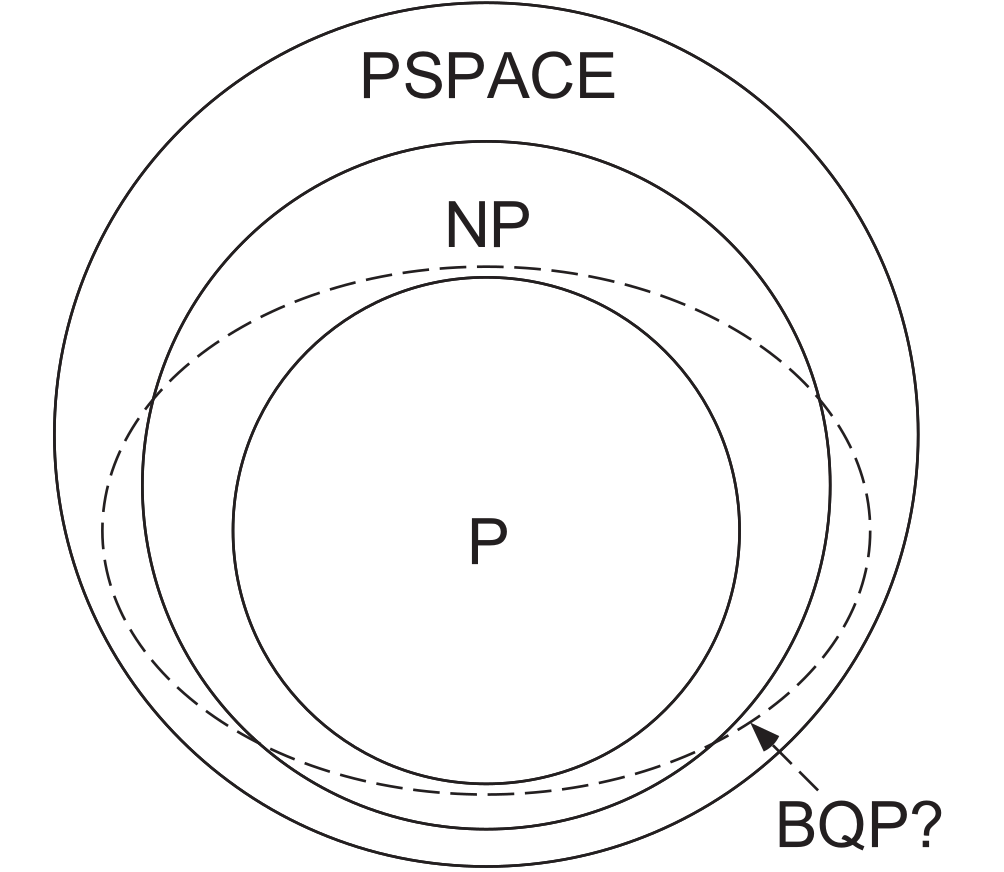
\includegraphics[width=0.6\textwidth]{images/bqp_pspace.png}
    \caption{We surely know that quantum computers can solve all \textbf{P} problems quickly and also that they cannot solve any problem outside \textbf{PSPACE} but we don't know where quantum computers fit between \textbf{P} and \textbf{PSPACE}. We don't even know whether \textbf{P} is equal to \textbf{PSPACE}.}
    \label{fig:bqp-pspace}
\end{figure}
We can already see that the \textit{theory} and notions of quantum computing pose a challenge to traditional computational methods. Another important challenge is that quantum computing is believed to be \textit{experimentally realizable}, primarily because nature works according to quantum mechanics.

\section{Experimental quantum information processing}
We'll look into experimentally proving that quantum computing can be done. Let's start with the "Stern-Gerlach" experiment which provides evidence to the existence of qubits in nature.
\subsection{The Stern-Gerlach experiment}
In the original experiment performed in 1921-22, hot `silver atoms' were beamed from an over through a magnetic field which deflected it. We'll consider the hydrogen atom version performed in 1927 as it's much simpler. A hydrogen atom consists of a proton and an electron spinning around which makes up the atomic dipole moment. By constructing the apparatus properly, it's possible to make the atom deflect by an amount dependent on the $\hat{z}$ component of atomic dipole moment. It's naturally expected that the atomic dipole moments would be randomly oriented and we'd get a continuous distribution. But the atoms were deflecting at specific angles. This was then explained by the \textit{quantization} principle, which was trending at that time. But quantum mechanics had predicted that the net atomic dipole of an atom must be zero, which is classically strange though, but there were two beams seen, one deflected up and the other deflected down.

This puzzle was explained by a new quantity called \textit{spin} which every hydrogen atom is supposed to be associated with. This spin is posited to make \textit{extra contribution} to the magnetic dipole moment.
\begin{figure}[H]
    \centering
    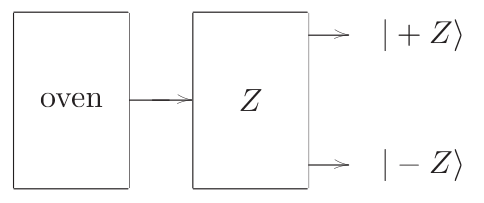
\includegraphics[width=0.4\textwidth]{images/stern_gerlach.png}
    \caption{Original Stern-Gerlach setup.}
    \label{fig:stern-gerlach}
\end{figure}
We can assume that the spins $\ket{+Z}$, $\ket{-Z}$ leads to upper and lower deflection respectively. Now if the apparatus modiied that the upper beam is then passed through another apparatus \textit{tipped sideways} so that it deflects according to $\hat{x}$ axis.


\part{Week 3}
\chapter{Quantum noise and quantum operations}
We'll be discussing about \textit{open systems}. These are unlike \textit{closed} systems, which don't interact with outside environment. These can suffer with unwanted interactions with the outside environment. These unwanted interations show up as \textit{noise} in quantum information systems. We'll describe \textit{quantum operations formalism}, a powerful set of tools enabling us to describe \textit{open} quantum systems and their behaviour. These can describe not only systems weakly coupled with the environment, but also the system which are strongly coupled with the environment. They can also describe closed systems which are suddenly opened and are subject to measurement. They are good at describing \textit{discrete} state changes, i.e changes of state from $\rho$ to $\rho'$ without explicit mention of passage of time. 

\section{Classical noise and Markov processes}
To understand about noise, let's consider a simple situation where a hard drive of a computer stores a single bit, which can be 0 or 1. Due to external stray magnetic fields, this bit is subject to change after a long time. To quantify it, let $p$ be the probability that the bit will flip, then $1-p$ will be the probability that the bit remains the same.
\begin{figure}[H]
    \centering
    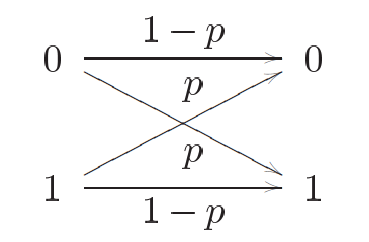
\includegraphics[width=0.3\textwidth]{images/classical_noise.png}
    \caption{A bit flip might occur with probability $p$}
    \label{fig:classical_noise}
\end{figure}
To figure out this probability $p$, we need to understand two things \begin{enumerate*}[label=(\alph*)]
\item How the magnetic fields are distributed in the enviroment. Assuming the owner isn't crazy and placing a magnet near the disk, we can sample the magnetic field near the disk similar to the one the disk is in.
\item How this environment's magnetic field interacts with the disk. This can be done by the well established \textit{Maxwell's equations}.
\end{enumerate*}

Suppose $p_0$, $p_1$ be the probabilities that the bit is in state 0 and 1 initially. Let $q_0, q_1$ be the corresponding probabilities after the noise has occured and $X, Y$ be the initial and final states respectively then
\begin{equation}
    P(Y=y) = \sum_x P(Y=y | X=x)P(X=x)
\end{equation}
where the conditional probability $P(Y=y | X=x)$ is known as the \textit{transition probability}. Thus
\begin{equation}
    \begin{bmatrix}
        q_0 \\ q_1
    \end{bmatrix}
    = \begin{bmatrix}
        1-p & p \\ p & 1-p
    \end{bmatrix}
    \begin{bmatrix}
        p_0 \\ p_1
    \end{bmatrix}
\end{equation}
Suppose we make a quantum circuit made of two faulty \textsc{not} gates. It takes an input state $X$ converts it into an intermediate bit $Y$ which is finally converted to $Z$. If we make a physically reasonable assumption that the noise produced at first \textsc{not} gate independent of the noise produced at the second \textsc{not} gate, it results in a stochastic process $X\longrightarrow Y\longrightarrow Z$ of a special type known as \textit{Markov process}. Often in multi-stage processes, it's a good assumption to use Markov processes. 

For a single stage process, output probabilities $\vv{q}$ are related to the input probabilities $\vv{p}$ according to
\begin{equation}
    \vv{q} = E\vv{p}
\end{equation}
$E$ is a matrix of transition probabilities known as the \textit{Evolution matrix}. Thus the final state of system is linearly related to it's initial state. This linearity is echoed in quantum noise's description, where probability distributions are replaced by density operators. In addition to this, $E$ follows two more rules
\begin{enumerate*}[label=(\alph*)]
    \item All of it's entries must be positive, so that $E\vv{p}$ is also positive and a valid probability distribution. This is known as \textit{positivity}.
    \item Sum of the entries in each column should be 1. This is known as \textit{completeness}.
\end{enumerate*}

\section{Quantum operations}
\subsection{Overview}
Quantum operations formalism is a general tool for describing evolution of quantum systems in a wide variety of circumstances, include stochastic changes, similar to how Markov processes describing classical stochastic changes. Similar to how classical bits are represented using probability distributions, here we'll use \textit{density operators}. The transformation looks like
\begin{equation}
    \rho' = \mathcal{E} (\rho)
\end{equation}
Here, $\rho$ is the initial density operator describing the state of the system. Similarly, $\rho'$ is the final state upto a normalization factor. A few known transforms $\mathcal{E}$ are unitary transformations and measurements $\mathcal{E}(\rho) = U\rho U^\dag$ and $\mathcal{E}_m(\rho) = M_m\rho M_m^\dag$.

In our further study, we're going to look at quantum operations \textit{three} seperate ways. The first way is based on the idea of studying dynamics as the result of interaction between a system and environment. This method is \textit{concrete} and easy to relate to real world. But it is mathematically inconvenient. Second way is euivalent to the first one but is mathematically convenient using a powerful mathematical representation for quantum operations known as the \textit{operator-sum representation}. Third way is equivalent to the first two, it's via a set of \textit{physically motivated axioms} that we'd expect these maps to satisfy. It's advanage is that it shows that quantum dynamics will be described by quantum operations in a wide range of circumstances. But this is neither concrete nor mathematically convenient. 
\begin{figure}[H]
    \centering
    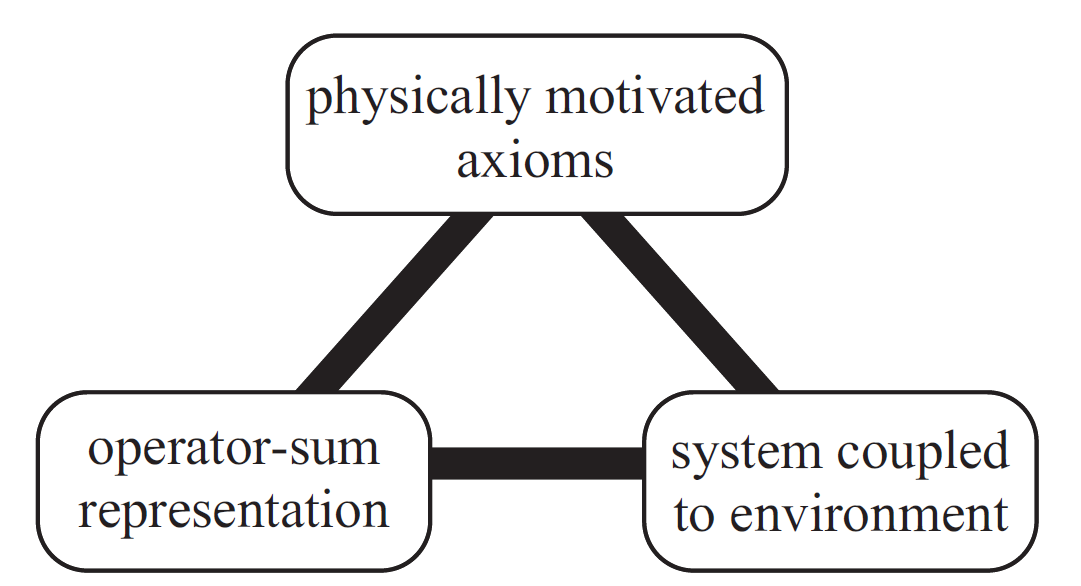
\includegraphics[width=0.6\textwidth]{images/quantum_operations.png}
    \caption{Three ways we're going to look at quantum operations, each provide their own advantages}
    \label{fig:quantum_operations}
\end{figure}

\subsection{Environment and quantum operations}
By the postulate of quantum mechanics, dynamics of a \textit{closed} system is described by just a unitary transform which can be thought of as a box. For dynamics of an \textit{open} system, the system can be thought of as a composite closed system of the system we're considering, \textit{principal system} and the \textit{environment}. 

Suppose the system is in state $\rho$, then the final state would be $\mathcal{E}(\rho)$ which need not be a unitary transform. We \textit{assume} that system and environtment are in a product state $\rho \otimes \rho_{env}$. Evolution of this closed system is described by a unitary transform $U$ and we use partial trace to find final state of the system $\mathcal{E}(\rho)$
\begin{equation}
    \mathcal{E}(\rho) = \text{tr}_{\text{env}} \left[ U\rho \otimes \rho_{\text{env}} U^\dag \right]
\end{equation}
This is the first \textit{definition} of quantum operations. If $U$ doesn't depend on the environment, then final state is simply $\Tilde{U}\rho \Tilde{U}^\dag$ where $\Tilde{U}$ is just part of transform on our principal state.

We assumed that environment and principal system are in a product state, but this might not be the case always. In cases of practical interest, this assumption is reasonable. The experimentalist while preparing an open state clears all the \textit{correlations} between the state and environment.

You might thin the envionment would have near-infinite dimensional Hilbert space, but it turns out that for principal system with $d$-dimensional Hilbert space, it's enough to model the environment with no more that $d^2$ dimensions.

\subsection{Operator sum representation}
How an open system evolves can be understood with an operator acting on the Hilbert space of principal system. This representation of quantum operations is known as \textit{Operator sum representation}.

Let this environment be in a pure state $\rho_{\text{env}} = \op{e_0}$, which even if it's not, can be made pure. Let $\ket{e_k}$ be an orthonormal basis for environment. The operation can be represented as
\begin{align}
    \mathcal{E}(\rho) &= \sum_k \bra{e_k} U\left[ \rho \otimes \op{e_0}) \right] U^\dag \ket{e_k} \\
    &= \sum_k E_k \rho E_k^\dag
\end{align}

where $E_k = \bra{e_k} U \ket{e_0}$ is an operator acting on principal state known as an \textit{operation element.} These have a nice property known as \textit{completeness relation} coming from the fact that $\tr{\mathcal{E}(\phi)} = 1$ since that's just another valid state
\begin{align}
    1 &= \tr{\mathcal{E}(\rho )} \\
    &= \text{tr}\left( \sum_k E_k \rho E_k^\dag \right) \\
    &= \text{tr} \left( \sum_k E_k E_k^\dag \rho \right)
\end{align}
As it's true for all $\rho$,
\begin{equation}
    \sum_k E_k E_k^\dag = I
\end{equation}
This is satisfied by operations which are \textit{trace-preserving}. We'll see later non trace preserving operations are also equivalent to this.

This representation gives us \textit{intrinsic} means to characterize dynamics of the principal system. We don't need to know how the environment works, just $E_k$ are sufficient.
Next up we'll see it's physical interpretation, making a physical model from this representation and also how to define this representation when our assumptions faii.

\subsubsection{Physical inerpretation of operator-sum representation}
Suppose a unitary transform $U$ is applied followed by a measurement of the environment, in basis $\ket{e_k}$. The measurement only affects the environment, thus state of the system if the output is $k$ is
\begin{align}
    \rho_k &\propto \text{tr}_E\left( \op{e_k}U(\rho \otimes \op{e_0}) U^\dag \op{e_k} \right) \\
    &= \bra{e_k} U\left( \rho \otimes \op{e_0}) \right) U^\dag \ket{e_k} \\
    &= E_k \rho E_k^\dag
\end{align}
which upon normalizing gives,
\begin{align}
    \rho_k = \frac{E_k\rho E_k^\dag}{\tr{E_k\rho E_k^\dag}}
\end{align}
with probability
\begin{equation}
    \tr{E_k\rho E_k^\dag}
\end{equation}
thus the final output is
\begin{align}
    \mathcal{E}(\rho) = \sum_k E_k\rho E_k^\dag
\end{align}

Thus we can see that a quantum operation changes the input randomly into a state $\frac{E_k\rho E_k^\dag}{\tr{E_k\rho E_k^\dag}}$ with probability $\tr{E_k\rho E_k^\dag}$ which is very similar to a noisy channel.

\subsubsection{Measurement and operator-sum representation}
We can have non trace preserving operations if we allow \textit{measurement} of the prinicpal state-environment system after the operator $U$ is applied. Suppose the principal system is represented by $Q$ and the environment by $E$, both are initially independent, environment is in the state $\sigma$. Then
\begin{equation}
    \rho^{QE} = \rho \otimes \sigma
\end{equation}
Now a unitary transform $U$ is applied, then a projective measurement is made using $P_m$. We assume no measurement is made is same as the outcome is $m=0$ and $P_0\equiv I$. The final state of $QE$ is
\begin{equation}
    \frac{P_m U(\rho \otimes \sigma) U^\dag P_m}{\tr{P_m U(\rho \otimes \sigma) U^\dag P_m}}
\end{equation}
State of only the principal system $Q$ is
\begin{equation}
    \frac{\text{tr}_E(P_m U(\rho \otimes \sigma) U^\dag P_m)}{\tr{P_m U(\rho \otimes \sigma) U^\dag P_m}}
\end{equation}
We can define a map $\mathcal{E}_m(\rho)$ as
\begin{equation}
    \mathcal{E}_m(\rho) = \text{tr}_E(P_m U(\rho \otimes \sigma) U^\dag P_m)
\end{equation}
therefore the final state of $Q$ is $\frac{\mathcal{E}_m(\rho)}{\tr{\mathcal{E}_m(\rho)}}$ and $\tr{\mathcal{E}_m(\rho)}$ is the probability of measurement outcome $m$. Suppose $\ket{e_k}$ is an orthonormal basis of $E$ and $\sigma=\sum_j q_j\ket{j}$ is an ensemble of initial state of environment then we observe that
\begin{align}
    \mathcal{E}_m(\rho) &= \sum_{jk} q_j\text{tr}_E(\op{e_k}P_m U(\rho \otimes \sigma) U^\dag P_m\op{e_k}) \\
    &= \sum_{jk} E_{jk} \rho E_{jk}^\dag
\end{align}
where
\begin{equation}
        E_jk \equiv \sqrt{q_j}\bra{e_j}U\ket{j}
\end{equation}
using which we can calculate the operators for the operator sum representation if $\sigma$ of $E$ is known. Even though we don't make projective measurements, respective measurement probabilities are $\tr{\mathcal{E}_m(\rho)}$

\subsubsection{System-environment models for any operator-sum representation}
Now a natural question is for a given set of operators $\{ E_k \}$ is it possible to find a reasonable \textit{model environment system and dynamics} which give rise to the quantum operation described by these operators. It turns out that for a set of trace preserving or non trace preserving quantum operation $\mathcal{E}$, there exists a model environment $E$ staring with a pure state $\ket{e_0}$, and model dynamics specified by unitary operator $U$ and projector $P$ onto $E$ such that
\begin{equation}
    \mathcal{E}(\rho) = \text{tr}_E(PU(\rho \otimes \op{e_0})U^\dag P)
\end{equation}

\subsection{Axiomatic approach to quantum operations}
We'll try to write down physically motivated axioms which quantum operations obey. We'll start over from scratch using these axioms. We'll then prove that a map $\mathcal{E}$ satisfies these axioms \textit{if and only if} it has an operator sum representation.

We \textit{define} a quantum operation $\mathcal{E}$ as a map from the set of density operators of the input space $Q_1$ to the set of density operators for the output space $Q_2$, which satisfy the following (for convenience we'd take $Q_1=Q_2=Q$):
\begin{enumerate}
    \item $\tr{\mathcal{E}(\rho)}$ denotes the probability that the map described by $\mathcal{E}$ occurs. Thus $0 \leq \tr{\mathcal{E}(\rho)} \leq 1$.
    \item $\mathcal{E}$ is a \textit{convex-linear map} on the set of density matrices i.e
    \begin{equation}
        \mathcal{E}\left( \sum_i p_i\rho_i \right) = \sum_i p_i\mathcal{E}(\rho_i).
    \end{equation}
    \item $\mathcal{E}$ is a \textit{completely-positive map} i.e $\mathcal{E}(A)$ is positive for any positive $A$. Also, if we introduce an extra system $\mathcal{R}$, then $\mathcal{I}\otimes \mathcal{E}(A) $ is positive for any positive $A$ in $\mathcal{R}Q_1$, where $\mathcal{I}$ is the identity map on $\mathcal{R}$.
\end{enumerate}

The following theorem binds the axiomatic approach and the operator-sum representation
\begin{theorem}
    The map $\mathcal{E}$ satisfies the above axioms if and only if
    \begin{equation}
        \mathcal{E}(\rho) = \sum_k  E_k\rho E_k^\dag
    \end{equation}
    for some set of operators $\{ E_k \}$ mapping the input Hilbert space to the output Hilbert space and satisfying $\sum_k E_k E_k^\dag \leq I$
\end{theorem}

\subsubsection{Freedom in the operator-sum representation}
A quanum operation can be described by two different set of operators. For example take $\mathcal{E}(\rho)=\sum_k E_k\rho E_k^\dag$ and $\mathcal{F}(\rho) = \sum_k F_k\rho F_k^\dag$ and
\begin{align}
    E_1 &= \frac{I}{\sqrt{2}} = \frac{1}{\sqrt{2}}\begin{bmatrix}
        1 & 0 \\ 0 & 1
    \end{bmatrix}
    &E_2 = \frac{Z}{\sqrt{2}} = \frac{1}{\sqrt{2}}\begin{bmatrix}
        1 & 0 \\ 0 & -1
    \end{bmatrix}
    \\
    F_1 &= \op{0} = \begin{bmatrix}
        1 & 0 \\ 0 & 0
    \end{bmatrix}
    &F_2 = \op{1} = \begin{bmatrix}
        0 & 0 \\ 0 & 1
    \end{bmatrix}
\end{align}

Understanding which sets of operations gives rise to same quantum operations is important for two reasons. \begin{enumerate*}[label=(\alph*)]
    \item Understanding the freedom in representation gives us more insight into how different physical processes give rise to same dynamics
    \item Understanding freedom in operator-sum representation is cruicial to a good understanding of quantum error-correction.
\end{enumerate*}
This is described usin the following theorem
\begin{theorem}[\textbf{Unitary freedom in the operator-sum representation}]
    Suppose $\{ E_1,\cdots, E_m \}$ and $\{ F_1, \cdots, F_n \}$ are operation elements giving rise to quantum operations $\mathcal{E}$ and $\mathcal{F}$ respectively. We may ensure $m=n$ by appending 0 operators to the end of shorter operation elements' list. Then $\mathcal{E}=\mathcal{F}$ if and only if there exist complex numbers $u_{ij}$ such that $E_i = \sum_j u_ij F_j$ and $u_{ij}$ is a unitary matrix.
\end{theorem}

This is similar to the result when two states are denoted by the same density operator. Using this theorem we can also answer the question, what is the maximum number of dimensions of an environment needed to mock up a quantum operation as described by this theorem.

\begin{theorem}
    All quantum operations $\mathcal{E}$ on a principal system of Hilbert space dimension $d$ can be generated by an operator sum representation containing atmost $d^2$ elements, i.e
    \begin{equation}
        \mathcal{E}(\rho) = \sum_{k=1}^M E_k\rho E_k^\dag
    \end{equation}
    where $1\leq M\leq d^2$.
\end{theorem}

\section{Examples of quantum noise and quantum operations}
\subsection{Trace and partial trace}
Quantum operations formalism can be used to describe a measurement, it's outcome and the state of the system after the measurement. The simplest such operation is related to the map $\rho \longrightarrow \tr{\rho}$. Let $H_Q$ be the input Hilbert space with orthogonal basis $\ket{1}, \cdots, \ket{d}$ and $H_Q'$ is a one dimensional Hilbert space, spanned by $\qo$, define $\mathcal{E}(\rho)$ as
\begin{equation}
    \mathcal{E}(\rho) \equiv \sum_{i=1}^{d} \qo \bra{i} \rho \ket{i} \bra{0}
\end{equation}
Do note that $\mathcal{E}(\rho) = \tr{\rho}\op{0}$, thus this quantum operation is identical to the trace operation, ignoring the factor of $\op{0}.$

Another interesting thing comes when we have a joint system $QR$ and we want to trace out $R$. Let $\ket{j}$ be the basis of $R$, let's define a linear operator $E_i: H_{QR} \longrightarrow H_Q$ as
\begin{equation}
    E_i\left( \sum_j \lambda_j \ket{q_j} \ket{j} \right) = \lambda_i \ket{q_i}
\end{equation}
when $\ket{q_j}$ are arbitrary vectors in $Q$ and $\lambda_j$ are just constants. Then we define a quantum operation as
\begin{equation}
    \mathcal{E}(\rho) \equiv \sum_k E_k\rho E_k^\dag
\end{equation}
We also notice that
\begin{equation}
    \mathcal{E}(\rho \otimes \ket{j}\bra{j'}) = \rho \delta_{j, j'} = \rho \tr{\ket{j}\bra{j'}} = \text{tr}_R(\rho \otimes \ket{j}\bra{j'}).
\end{equation}
where $\ket{j}, \ket{j'}$ are members of orthonormal basis of $R$. Thus, by linearity of $\mathcal{E}$ and $\text{tr}_R$ we have $\mathcal{E} = \text{tr}_R$
\subsection{Geometric picture of single qubit quantum operations}
We've seen before that a single qubit's density operator can be represented by
\begin{equation}
    \rho = \frac{I+\Vec{r} \cdot \Vec{\sigma}}{2}
\end{equation}
where $\Vec{r}$ is a three dimensional real unit vector and $\Vec{\sigma}$ is a vector of pauli matrices. Thus
\begin{equation}
    \rho = \frac{1}{2}\begin{bmatrix}
        1+r_z & r_x-ir_y \\ r_x+ir_y & 1-r_z
    \end{bmatrix}
\end{equation}
Using this representation, it can be shown that an arbitrary trace-preserving quantum operation is equivalent to the map
\begin{equation}
    \Vec{r} \longrightarrow \Vec{r}' = M\Vec{r} + \Vec{c}
\end{equation}
where $M$ is a $3\times 3$ real matrix, and $\Vec{c}$ is a constant vector. This is an \textit{affine map}, mappping Bloch sphere into itself. To see this, suppose the operators $E_i$ generating $\mathcal{E}$ are written in the form
\begin{equation}
    E_i = \alpha_i I + \sum_{k=1}^3 a_ik\sigma_k
\end{equation}
Then it can be checked that
\begin{align}
    M_{jk} = \sum_l \left[ a_{lj}a_{lk}^* + a_{lj}^*a_{lk} + \left( |\alpha_l|^2 - \sum_p a_{lp}a_{lp}^* \right) \delta_{jk} + i\sum_p \epsilon_{jkp}(\alpha_la_{lp}^* - \alpha_l^*a_{lp}) \right] 
\end{align}
\begin{align}
    c_k = 2i \sum_l \sum_{jp}\epsilon_{jpk}a_{lj}a_{lp}^*
\end{align}
The affine map can be better understood by te polar decomposition of $M$ into $M=U|M|$, where $U$ is unitary. Since $M$ is real, $|M|$ is real and hermitian, i.e a symmetric matrix. Thus, as $M$ is real, we may assume $U$ is real, and an orthogonal matrix i.e $U^TU=I$ Thus, we can write
\begin{equation}
    M = OS
\end{equation}
where determinant of $O$ is 1 and it's an orthogonal matrix describing rotation. $S$ is a real symmetric matrix. Thus the above equation can be understood as the deformation of the bloch sphere about axis as specified by $S$ followed by a rotation defined by $O$, then a displacment due to $\Vec{c}$.
\subsection{Bit flip and phase flip channels}
Suppose we take a single qubit and pass it through a noisy \textit{bit-flip} channel, which flips the state of a qubit from $\qo$ to $\qi$ with probability $1-p$. It has operation elements
\begin{align}
    &E_0 = \sqrt{p}I = \sqrt{p}\begin{bmatrix}
        1 & 0 \\ 0 & 1
    \end{bmatrix}
    &E_1 = \sqrt{1-p}X = \sqrt{1-p}\begin{bmatrix}
        0 & 1 \\ 1 & 0
    \end{bmatrix}
\end{align}
This affects the bloch vector in the following way:
\begin{figure}[H]
    \centering
    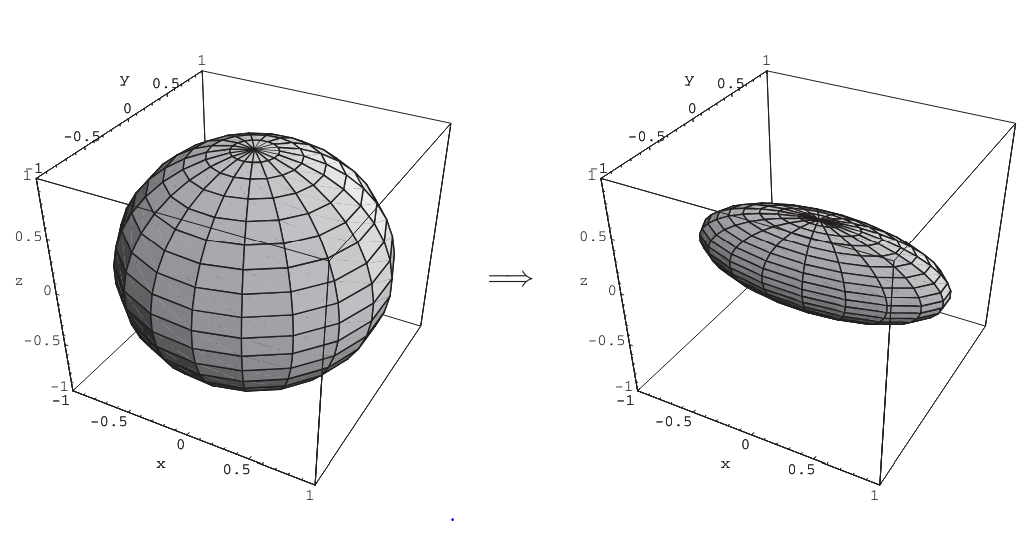
\includegraphics[width=\textwidth]{images/bit_flip_bloch.png}
    \caption{Bit flip channl. The operation doesn't affect the $x$ component, but shrinks the $y$ and $z$ component by a factor of $1-2p$. Here $p=0.3$.}
    \label{fig:bit_flip_bloch}
\end{figure}
It's easy to verify that $\tr{\rho^2}=\frac{1+|\Vec{r}|^2}{2}$. Thus, this operation can never increase the length of Bloch vector i.e can never increase $\tr{\rho^2}$. Thus the purity of $\rho$ is always decreased by this. Thus Bloch sphere provides an intuitive way of understanding quantum operations.   

Similarly if we consider the \textit{phase-flip} channel which has operation elements
\begin{align}
    &E_0 = \sqrt{p}I = \sqrt{p}\begin{bmatrix}
        1 & 0 \\ 0 & 1
    \end{bmatrix}
    &E_1 = \sqrt{1-p}Z = \sqrt{1-p}\begin{bmatrix}
        1 & 0 \\ 0 & -1
    \end{bmatrix}
\end{align}
we see that the following transformation is happening to the Bloch sphere.
\begin{figure}[H]
    \centering
    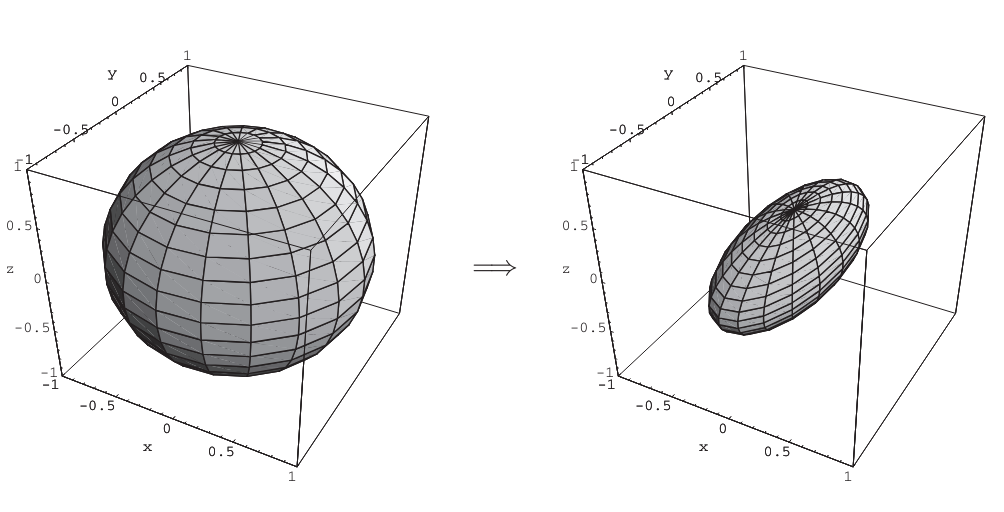
\includegraphics[width=\textwidth]{images/bit_phase_flip_bloch.PNG}
    \caption{Phase flip channel. As we can see, it does nothing to the $z$ component, but shrinks $x$ and $y$ component by a factor of $1-2p$. Here p=0.3.}   
    \label{fig:phase_flip_bloch}
\end{figure}
As a special case when $p=0.5$, using the freedom in the operator-sum representation, this operation can be written as
\begin{equation}
    \rho \longrightarrow \mathcal{E}(\rho) = P_0\rho P_0 + P_1\rho P_1
\end{equation}
which is nothing but the measurement with respect to the basis $\qo, \qi$, the result unknown. The corresponding map on Bloch sphere here is 
\begin{equation}
    (r_x,r_y,r_z) \longrightarrow (0,0,r_z)
\end{equation}
i.e the Bloch vector is projected along $z$ axis loosing $x$ and $y$ components.

The \textit{bit-phase flip} channel has the operation elements
\begin{align}
    &E_0 = \sqrt{p}I = \sqrt{p}\begin{bmatrix}
        1 & 0 \\ 0 & 1
    \end{bmatrix}
    &E_1 = \sqrt{1-p}Y = \sqrt{p}\begin{bmatrix}
        0 & -i \\ i & 0
    \end{bmatrix}
\end{align}
when this operation is done, the $y$ component of the Bloch sphere remain intact. Whereas $x,z$ components are shrinked by a factor of $1-2p$ as shown
\begin{figure}[H]
    \centering
    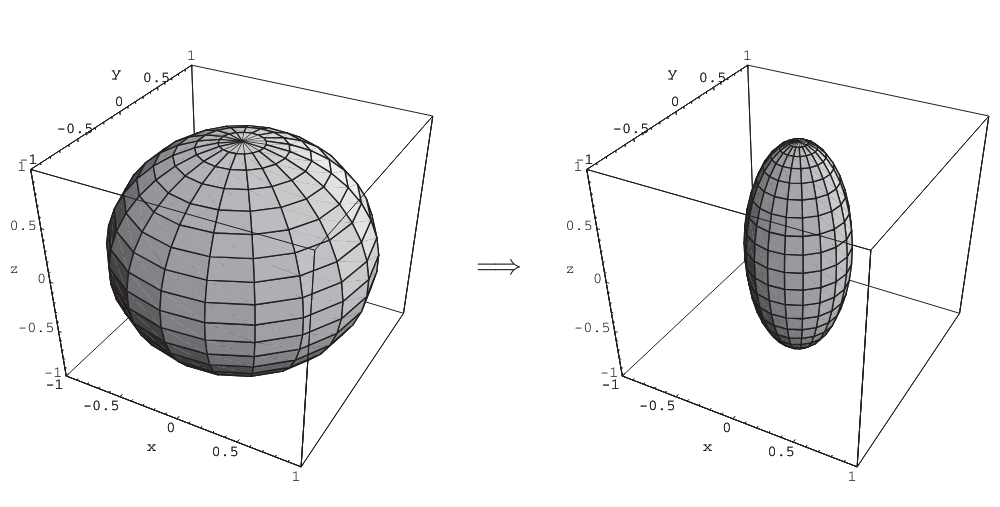
\includegraphics[width=\textwidth]{images/phase_flip_bloch.PNG}
    \caption{Bit-phase flip channel. Here p=0.3, it can e seen that $y$ axis remains intact while $x$ and $z$ axes are shrinked by a factor of $1-2p$.}
    \label{fig:bit_phase_flip_bloch}
\end{figure}
\subsection{Depolarizing channel}
It's an important type of quantum noise channel. We take a single qubit, and with probability $p$ the qubit is \textit{depolarized} i.e replaced by a completely mixed state $\frac{I}{2}$ or left untouched with probability $1-p$. Thus the state of the qubit after noise is
\begin{equation}
    \E{\rho} = \frac{pI}{2} + (1-p)\rho
    \label{eq:depolarizing_channel}
\end{equation}
The effect on Bloch sphere is as shown
\begin{figure}[H]
    \centering
    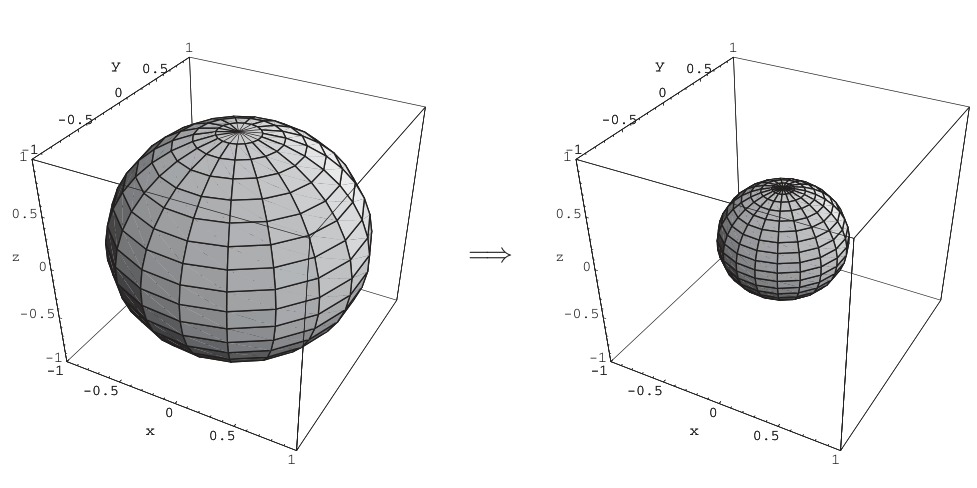
\includegraphics[width=0.9\textwidth]{images/depolarizing_bloch.png} 
    \caption{Effect of depolarizing channel on the Bloch sphere}
    \label{fig:depolarizing_bloch}
\end{figure}
The quantum circuit depicting the depolarizing channel is
\begin{figure}[H]
    \centering
    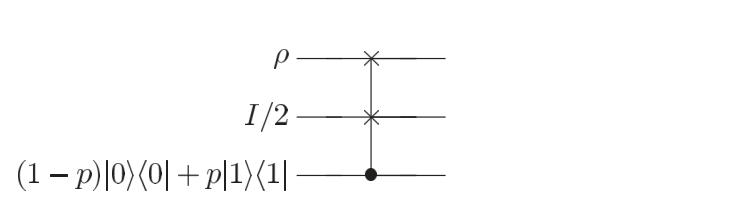
\includegraphics[width=0.7\textwidth]{images/depolarizing_circuit.png}
    \caption{Quantum circuit representing the depolarizing channel}
    \label{fig:depolarizing-circuit}
\end{figure}
The third qubit is qubit is a mixture of state $\qo$ and $\qi$ with probability $p$ and $1-p$ respectively. This is responsible for the second qubit getting swapped into the first qubit. In \ref{eq:depolarizing_channel}, $I/2$ can be represented as
\begin{equation}
    \frac{I}{2} = \frac{\rho + X \rho X + Y \rho Y + Z \rho Z}{4}
\end{equation}
Thus \ref{eq:depolarizing_channel} becomes
\begin{equation}
    \E{\rho} = \left( 1-\frac{3p}{4} \right) \rho + \frac{p}{4}\left( X \rho X + Y \rho Y + Z \rho Z \right)
\end{equation}
Here the operation elements will be $\sqrt{1-3p/4}I$, $\sqrt{p}X/2$, $\sqrt{p}Y/2$, $\sqrt{p}Z/2$. Note that it is convenient to parametrize the depolarizing channel in different ways. The operation elements would differ, such as
\begin{equation}
    \E{\rho} = (1-p)\rho + \frac{p}{3}\left(X \rho X + Y \rho Y + Z \rho Z \right)
\end{equation}
Here, this does nothing with probability $1-p$ and applies $X$, $Y$ or $Z$ gates with probability $p/3$ each.

The depolarizing channel can be generalized for systems with dimensionality greater than 2. Suppose a system has dimension $d$ the quantum operation would become
\begin{equation}
    \E{\rho} = \frac{pI}{d} + (1-p)\rho
\end{equation}
\subsection{Amplitude damping}
The process of \textit{amplitude damping} helps us understand \textit{energy dissipation} in quantum systems. For example, to describe dynamics of an atom emitting a photon, how a spin system at high temperature reaches equilibrium with it's environment etc. What's common in these examples is described by a quantum operation known as \textit{amplitude damping}, which can be derived as follows. Suppose we have an optical mode at state $a\qo+b\qi$ which is superposition of zero or one photon. The scattering of a photon can be now described as keep a partially silvered mirror (a beamsplitter) in the path of the photon. It couples with another single optical node (it's environment) according to unitary transform $B = \exp{\left[ \theta(a^\dag b - ab^\dag \right]}$. Where $a$, $a^\dag$ and $b$, $b^\dag$ are annihilation and creation operators for photons in two modes. The output after beamsplitter assuming there's no photon in the environment is $B\qo(a\qo+b\qi) = a\ket{00} + b(\cos{\theta}\ket{01} + \sin{\theta}\ket{10}$. Tracing out the environment gives us the quantum operation
\begin{equation}
    \mathcal{E}_{AD}(\rho) = E_0\rho E_0^\dag + E_1\rho E_1^\dag
\end{equation}
where $E_k=\bra{e_k}0\ket{e_0}$ are
\begin{align}
    E_0 &= \begin{bmatrix}
        1 & 0 \\ 0 & \sqrt{1-\gamma}
    \end{bmatrix} \\
    E_1 &= \begin{bmatrix}
        0 & \sqrt{\gamma} \\ 0 & 0
    \end{bmatrix},
\end{align}
the operations elements for amplitude damping. $\gamma = \sin^2(\theta)$ can be thought of as the probability of loosing a photon. $E_1$ operation changes the state $\qi$ to $\qo$, this corresponds to the loss of quantum of energy to the environment. $E_0$ leaves $\qo$ unchanged but reduces the amplitude of $\qi$, this happens because there's no loss of quantum of energy, thus the environment perceives it to be more likely that the system is in $\qo$ state.
\begin{figure}[H]
    \centering
    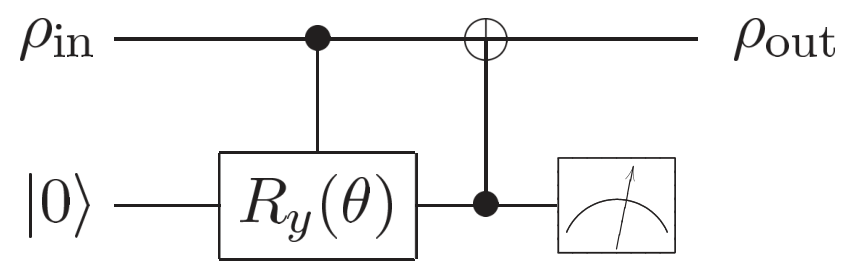
\includegraphics[width=0.6\textwidth]{images/amplitude_damp_circuit.png}
    \caption{This models an amplitude damping circuit with $\gamma = \sin^2(\theta/2)$}
    \label{fig:amplitude_damp_circuit}
\end{figure}
A general characteristic of a quantum operation is the set of states that are left invariant under the operation, as we've seen before. Here, $\qo$ is left invariant, but that is a cause of us assuming that the environment is starting at $\qo$ state, as if it were at \textit{zero temperature}.

The quantum operation defining amplitude damping at a finite temperature is known as \textit{generalized amplitude damping}, $\mathcal{E}_{\text{GAD}}$ and is defined for single qubits using operation elements
\begin{align}
    E_0 &= \sqrt{p}\begin{bmatrix}
        1 & 0 \\ 0 & \sqrt{1-\gamma}
    \end{bmatrix}
    &E_1 = \sqrt{p}\begin{bmatrix}
        0 & \sqrt{\gamma} \\ 0 & 0
    \end{bmatrix}
    \\
    E_2 &= \sqrt{1-p}\begin{bmatrix}
        \sqrt{1-\gamma} & 0 \\ 0 & 1
    \end{bmatrix}
    &E_3 = \sqrt{1-p}\begin{bmatrix}
        0 & 0 \\ \sqrt{\gamma} & 0
    \end{bmatrix}
\end{align}
and the stationary state $\rho_\infty$ satisfies $\E{\rho_\infty} = \rho_\infty$. This  GAD describes `$T_1$' relaxation processes due to coupling of spin to their surrounding lattice, a large system which is in thermal equilibrium at a temperature much higher than the spin temperature. This thing is useful in NMR quantum computation.

The effect of amplitude damping on Bloch sphere is 
\begin{equation}
    (r_x, r_y, r_z) \longrightarrow \left(r_x\sqrt{1-\gamma}, r_y\sqrt{1-\gamma}, \gamma+r_z(1-\gamma)\right)
\end{equation}
where $\gamma$ is replaced with a time varying function like $1-e^{-t/T_1}$ ($t$ is time and $T_1$ characterizes speed of the process). Using this we can visualize the effects as \textit{flow} on the Bloch sphere, where every point moves towards a fixed point, something like north pole where $\qo$ is located.

Similarly, generalized amplitude damping performs the transformation
\begin{equation}
    (r_x, r_y, r_z) \longrightarrow \left( r_x\sqrt{1-\gamma}, r_y\sqrt{1-\gamma}, \gamma(2p-1) + r_z(1-\gamma) \right)
\end{equation}
Generalized ammplitude damping is different than amplitude damping only in the location of fixed point of flow; the final state is along $\hat{z}$ axis, at the point $(2p-1)$, which is a mixed state.
\begin{figure}[H]
    \centering
    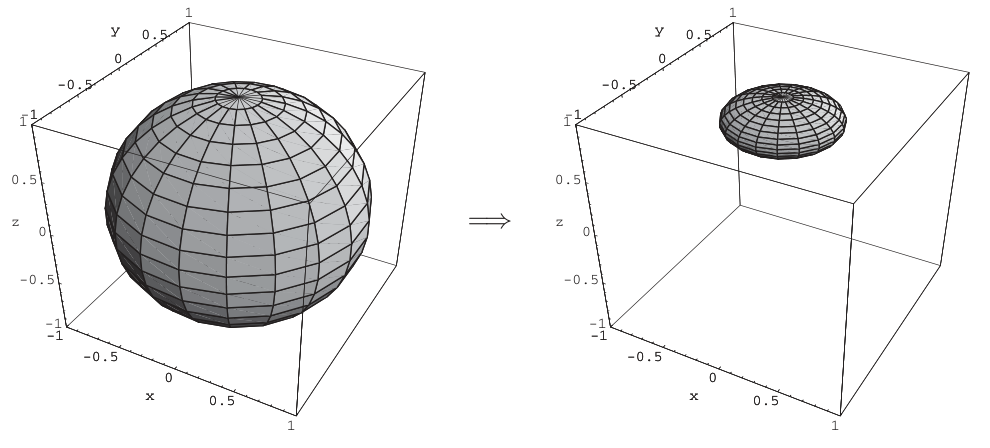
\includegraphics[width=\textwidth]{images/gad_bloch.png}
    \caption{The effect of amplitude damping channel on Bloch sphere, for $p=0.8$. Note how the entire sphere shrinks towards the north pole, the $\qo$ state.}
    \label{fig:gad_bloch}
\end{figure}

\subsection{Phase damping}
A noise process which is uniquely quantum mechanical, describes \textit{loss of quantum information} without \textit{loss of energy}, is \textit{\textbf{phase damping}}. For example it describes what happens when a photon scatters randomly as it travels through a waveguide, or how electronic states in an atom are perturbed upon interacting with distant electrical charges. The energy eigenstates don't change as a function of time but accumulate a phase proportional to the eigenvalues. When a system evolves for an amount of time not known, information about this quantum phase - the \textit{relative} phases between the eigenstates is lost.
\part{Week 4}
\chapter{Distance measures for quantum information}
We'll try to quantify how two information items are similar, how information is preserved over a process etc. For this, we'll define two classes \textit{distance measures}, \textit{static distance} which is how close two quantum states are, and \textit{dynamic distance} which is how well information is stored over a process. We'll define static distance properly first then build up dynamic distnance with it. Two widely used distance measures currently are \textit{trace distance} and \textit{fidelity}.

\section{Distance measures for classical information}
\textit{Hamming distance} is defined to quantify distance between two bit strings. It's equal to number of mismatching bits (eg. $\text{Hamming}(1011,0010)=2$. But this relies on labelling which we don't have in our Hilbert space arena of quantum mechanics.

We can define a classical information source as a random variable over the set of possible outcomes. So we know the probabilities of getting a given output. In this notion, we can compare two information sources with same index set using a distance measure known as \textit{trace distance}, defined as
\begin{equation}
    D(p_x, q_x) = \frac{1}{2}\sum_x |p_x-q_x|
\end{equation}
where $\{ p_x \}$ and $\{ q_x \}$ are probability distributions of both sources. This is also known as the \textit{$L_1$ distance} or \textit{Kolmogorov distance}. Trace because we use trace when we define this for quantum systems. This is a metric since it satisfies symmetricity ($D(x,y)=D(y,x)$) and triangle inequality ($D(x,y)\leq D(x,z)+D(y,z)$.

\textit{Fidelity}, a second measure is described by
\begin{equation}
    F(p_x, q_x) = \sum \sqrt{p_xq_x}
\end{equation}
This is not a metric as shown by it's physical interpretation in figure \ref{fig:fidelity-distance}.
\begin{figure}
    \centering
    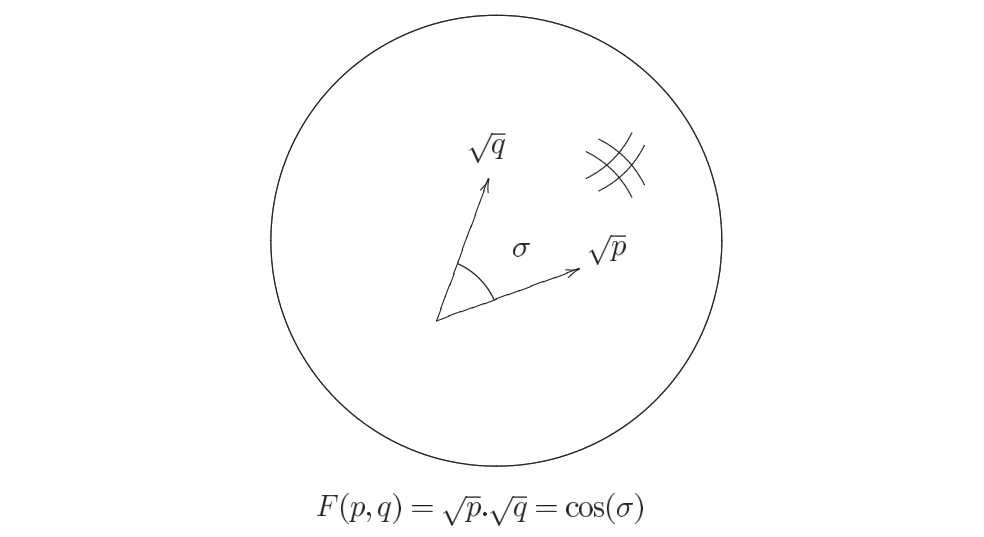
\includegraphics[width=0.9\textwidth]{images/fidelity_distance.png}
    \caption{$F(p_x,q_x)$ can be seen as dot product between $\sqrt{p}$ and $\sqrt{q}$, each of them lie on a unit sphere since $\sum_x \left( \sqrt{p_x} \right)^2 = 1$ and $\sum_x \left( \sqrt{q_x} \right)^2 = 1$}
    \label{fig:fidelity-distance}
\end{figure}

A physically motivated operational meaning for trace distance which can be proved is,
\begin{equation}
    D(p_x, q_x) = \max_S |p(S) - q(S)| = \max_S \left| \sum_{x\in S} p_x - \sum_{x \in S} q_x \right|
\end{equation}
which is maximum over all subsets over index set. This makes sense because $S$ represents an event which produces maximum difference in outputs. It can also be shown that the absolute value is redundant, i.e
\begin{equation}
    D(p_x, q_x) = \max_S \left( \sum_{x\in S} p_x - \sum_{x \in S} q_x\right)
\end{equation}
Trace distance and fidelity are static distance measures.

For \textit{dynamic measure} of distance, suppose a random variable $X$ is passed through a noise channel to produce $Y$ shown by Markov process $X\longrightarrow Y$, a dynamic measure showing how much information is preserved is $p(X\neq Y)$. This can be done using trace distance, for which let's construct a copy $\Tilde{X}$ of $X$ which is also a random variable. Now $X$ is passed through the channel, leaving output $Y$. The closeness between initial perfectly correlated pair $(\Tilde{X}, X)$ and the pair $(\Tilde{X}, Y)$ can be shown to be
\begin{equation}
    D((\Tilde{X},X), (X, Y)) = p(X\neq Y)
    \label{eq:trace_distance_using_copy}
\end{equation}
This thing we did to calculate $p(X\neq Y)$ is unique to classical mechanics. We can't \textit{directly} calculate quantum analogue of $p(X\neq Y)$ if $X$ and $Y$ exist at different times. We use quantum entanglement to define dynamic measure similar to the construction shown above. 
\begin{figure}[H]
    \centering
    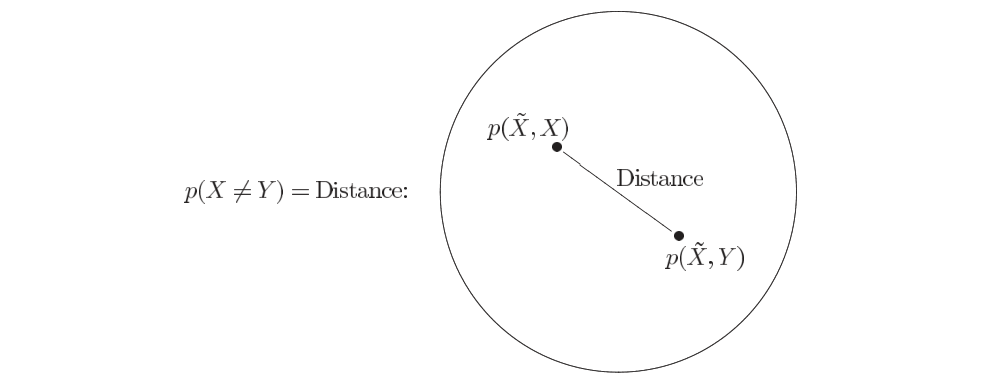
\includegraphics[width=0.8\textwidth]{images/dynamic_measure.png}
    \caption{The probability of an error in the channel is equal to the trace distance between the probability distributions for $( \Tilde{X}, X)$ and $( \Tilde{X}, Y )$.}
    \label{fig:dynamic_measure}
\end{figure}

\section{How close are two quantum states}
We'll see quantum generalizations of trace distance and fidelity.
\subsection{Trace distance}
\textit{Trace distance} between two quantum states $\rho$ and $\sigma$ is defined as
\begin{equation}
    D(\rho, \sigma) = \frac{1}{2}\text{tr} |\rho-\sigma|
\end{equation}
here $|A|=\sqrt{A^\dag A}$. If $\rho$ and $\sigma$ commute (matrix multiplication), this reduces to classical trace distance. Suppose $\rho$ and $\sigma$ commute, then
\begin{align}
    \rho = \sum_i r_i \op{i};
    \ \ \ 
    \sigma = \sum_i s_i \op{i}
\end{align}
for orthogonal basis $\ket{i}$. Then trace distance becomes
\begin{align}
    D(\rho, \sigma) &= \frac{1}{2}\text{tr}|\rho-\sigma| \\
    &= \frac{1}{2}\text{tr}|(r_i-s_i)\op{i}| \\
    &= D(r_i, s_i)
\end{align}
For qubits in Bloch sphere representation, it becomes nicer. Let
\begin{align}
    \rho = \frac{1+\Vec{r}\Vec{\sigma}}{2};
    \ \ \ 
    \sigma = \frac{1+\Vec{s}\Vec{\sigma}}{2}
\end{align}
then trace distance between $\rho$ and $\sigma$ is
\begin{align}
    D(\rho, \sigma) = \frac{|\Vec{r}-\Vec{s}|}{2}
\end{align}
using the fact that $(\Vec{r}-\Vec{s})\cdot \Vec{\sigma}$ has eigen values $\pm |\Vec{r}-\Vec{s}|$. It can be shown that

\begin{equation}
    D(\rho, \sigma) = \max_P \tr{P(\rho-\sigma)}
\end{equation}
where maximum is over all positive operators $P$, $P\leq I$.

\begin{theorem}
    Let $\{ E_m \}$ me a POVM, with $p_m \equiv \tr{\rho E_m}$ and $q_m \equiv \tr{\sigma E_m}$ be the probability of getting output labelled by $m$. Then
    \begin{equation}
        D(\rho, \sigma) = \max_{\{ E_m \} } D(p_m, q_m)
    \end{equation}
    where maximization is over all POVMs $\{ E_m \}$.
\end{theorem}
It can be shown that this trace distance is also a metric. Here goes another nice theorem

\begin{theorem}
    Suppose $\mathcal{E}$ is a trace preserving quantum operation. Let $\rho$, $\sigma$ be density operators. Then
    \begin{equation}
        D(\E{\rho}, \E{\sigma}) \leq D(\rho, \sigma)
    \end{equation}
\end{theorem}
Thus there exists no physical processes which increases distance between two states.
\begin{figure}[H]
    \centering
    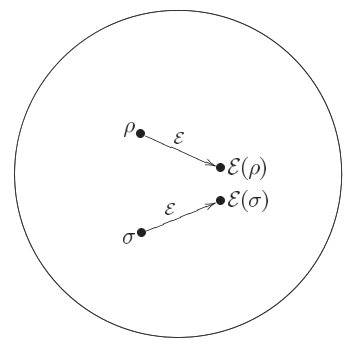
\includegraphics[width=0.4\textwidth]{images/contraction_due_to_operation.png}
    \caption{Trace-preserving quantum operations cause a contraction on the space of density operators.}
    \label{fig:contraction_due_to_operation}
\end{figure}

It can also be showed that
\begin{align}
    D(\rho^A, \sigma^A) \leq D(\rho^{AB}, \sigma^{AB})
\end{align}
intuitively, it's  like things are less differentiable if corresponding parts of them are covered.

\begin{theorem}[\textbf{Strong convexity of trace distance}]
    Let $\{ p_i \}$ and $\{ q_i \}$ be two probability distributions over the same index set, and $\rho_i$, $\sigma_i$ be density operators, also with indices from same index set, then
    \begin{equation}
        D\left( \sum_i p_i\rho_i, \sum_i q_i\sigma_i \right)
        \leq
        D(p_i, q_i) +
        \sum_i p_i D(\rho_i, \sigma_i)
    \end{equation}
    where $D(p_i, q_i)$ is the trace distance between the probability distributions $p_i$ and $q_i$.
\end{theorem}
using this we can show convexity properties of trace distance,
\begin{equation}
    D\left( \sum_i p_i\rho_i , \sigma \right)
    \leq
    \sum_i p_iD(\rho_i, \sigma)
\end{equation}
Also, any trace-preserving quantum operation $\mathcal{E}$ has a fixed point $\rho$ such that $\E{\rho} = \rho$.

\subsection{Fidelity}
\textit{Fidelity} is not a metric on  density operators but does give rise to a useful metric. Fidelity of state $\rho$ and $\sigma$ is defined as
\begin{equation}
    F(\rho, \sigma) \equiv \text{tr}\sqrt{\rho^{1/2}\sigma \rho^{1/2}}
\end{equation}
when $\rho$ and $\sigma$ commute, then
\begin{align}
    \rho = \sum_i p_i\op{i};
    \ \ \ \ 
    \sigma = \sum_i s_i\op{i}
\end{align}
for orthoonormal basis $\ket{i}$, we see that
\begin{align}
    F(\rho, \sigma) &= \text{tr}\sqrt{\sum_i r_is_i\op{i}} \\
    &= \text{tr}\left( \sum_i\sqrt{r_is_i}\op{i} \right) \\
    &= \sum_i \sqrt{r_is_i} \\
    &= F(r_i, s_i)
\end{align}
thus, when $\rho$ and $\sigma$ commute, quantum fidelity reduces to classical fidelity between eigenvalue distributions $r_i$, $s_i$ of $\rho$, $\sigma$ respectively. Also the fidelity between a pure state $\qv$ and an arbitrary state $\rho$ is
\begin{align}
    F(\qv, \rho) &= \text{tr}\sqrt{\bra{\psi}\rho\qv \qv \bra{\psi}} \\
    &= \sqrt{\bra{\psi}\rho\qv}
\end{align}
i.e fidelity is square root of overlap between $\qv$ and $\rho$.

There's no similar Bloch sphere representation for fidelity but it does satisfy similar properties like \textit{invariance under unitary transformation} i.e
\begin{align}
    F(U\rho U^\dag, U\sigma U^\dag) = F(\rho, \sigma)
\end{align}

\begin{theorem}[\textbf{Uhlmann's theorem}]
    Suppose $\rho$, $\sigma$ be states of a system $Q$, Let $R$ be a copy of $Q$. Then
    \begin{equation}
        F(\rho, \sigma) = \max_{\qv, \ket{\varphi}} \left| \braket{\psi | \varphi} \right|
    \end{equation}
    where the maximization is over all purifications $\qv$ of $\rho$ and $\ket{\varphi}$ of $\sigma$.
\end{theorem}

\begin{lemma}
    Let $A$ be any operator, $U$ be unitary. Then
    \begin{equation}
        |\tr{AU}| \leq |\tr{A}|
    \end{equation}
    equality is when $U=V^\dag$ when $A=|A|V$ is polar decomposition of $A$.
\end{lemma}
By Uhlmann's formula it can be shown that fidelity is \textit{symmetric} in its inputs i.e $F(\rho, \sigma) = F(\sigma, \rho)$ and also that it's bound, $0 \leq F(\rho, \sigma) \leq 1$. Also $\rho=\sigma \implies F(\rho, \sigma)=1$ else it's less than 1. Quantum fidelity is related to classical fidelity in the following way:
\begin{equation}
    F(\rho, \sigma) = \min_{E_m} F(p_m, q_m)
\end{equation}
where $E_m$ are POVMs, $p_m = \tr{\rho E_m}$, $q_m = \tr{\sigma E_m}$ are probability distributions corresponding to the POVM $\{ E_m \}$. 

We can define \textit{angle} between states $\rho$ and $\sigma$ by
\begin{equation}
    A(\rho, \sigma) = \arccos{F(\rho, \sigma)}
\end{equation}
This is non-negative, symmetric in inputs and zero when $\rho = \sigma$. It can be shown to satisfy triangle inequality, and thus is a metric.
\begin{figure}[H]
    \centering
    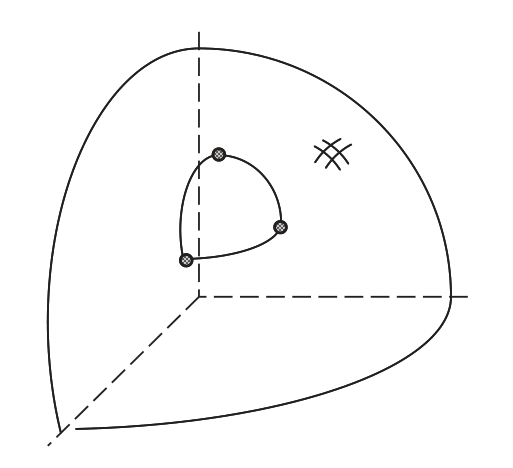
\includegraphics[width=0.5\textwidth]{images/fidelity_angle.png}
    \caption{Angle between unit vectors is a metric}
    \label{fig:fidelity-angle}
\end{figure}
Qualitatively, fidelity behaves like "upside down" of trace distance. It decreases as two states become more distinguishable and vice versa. Fidelity in \textit{non decreasing} as shown by the theorem
\begin{theorem}[\textbf{Monotonicity of fidelity}]
    Suppose $\rho$, $\sigma$ be density operators, and $\mathcal{E}$ is a trace-preserving operation, then
    \begin{equation}
        F(\E{\rho}, \E{\sigma}) \geq F(\rho, \sigma)
    \end{equation}
\end{theorem}
Angles we've defined above follow \textbf{contractivity} which is $A(\E{\rho}, \E{\sigma}) \leq A(\rho, \sigma)$, there's also \textit{strong concavity} of fidelity like trace distance
\begin{theorem}[\textbf{Strong concavity of fidelity}]
    Let $p_i$, $q_i$ be probability distributions over the same index set, $\rho_i$, $\sigma_i$ also indexed by the same index set. Then 
    \begin{equation}
        F \left( \sum_i p_i\rho_i, q_i\sigma_i \right)
        \geq
        \sum_i \sqrt{p_iq_i}F(\rho_i, \sigma_i)
    \end{equation}
\end{theorem}

\subsection{Relationships between distance measures}
Despite their different forms, trace distance and fidelity are closely related. In pure states, they're completely equivalent to each other, to see this consider two pure state $\ket{a}$ and $\ket{b}$, using Gram-schmidt we can find states $\qo$ and $\qi$ such that $\ket{a} = \qo$ and $\ket{b}=\cos{\theta}\qo + \sin{\theta}\qi$. Then $F(\ket{a}, \ket{b}) = |\cos{\theta} |$ and
\begin{align}
    D(\ket{a}, \ket{b}) &= \frac{1}{2}\text{tr} \left|
     \begin{bmatrix}
         1-\cos^2\theta & -\cos{\theta}\sin{\theta} \\
         -\cos{\theta}\sin{\theta} & -\sin^2\theta
     \end{bmatrix} 
    \right|
    \\
    &= |\sin{\theta}| \\
    &= \sqrt{1-F(\ket{a}, \ket{b})^2}    
\end{align}
For mixed states $\rho$, $\sigma$ let $\qv$ and $\ket{\varphi}$ be purifications of $\rho$, $\sigma$ such that $F(\rho, \sigma) = |\braket{\psi | \varphi}| = F(\qv, \ket{\varphi})$. Since trace distance is non-increasing under the partial trace,
\begin{align}
    D(\rho, \sigma) &\leq D(\qv, \ket{\varphi}) \\ 
    &= \sqrt{1-F(\rho, \sigma)^2}
\end{align}
It can be further shown that
\begin{equation}
    1-F(\rho, \sigma) \leq D(\rho, \sigma) \leq \sqrt{1-F(\rho, \sigma)^2}
\end{equation}

\section{How well does a quantum channel preserve information?}
We'll try to quantify how much that state has "changed" from $\qv$ to $\E{\op{\psi}}$ due to an operation $\mathcal{E}$ using the distance measures discussed. Let's look at a simple example how a state changes under depolarizing channel using fidelity
\begin{align}
    F(\qv, \E{\op{\psi}}) &= \sqrt{\bra{\psi}
    \left( p\frac{I}{2} + (1-p)\op{\psi} \right) \qv
    }\\
    &= \sqrt{1-\frac{p}{2}}
\end{align}
it can be clearly seen when we reduce $p$, fidelity get's close to one hence the states becoming more indistinguishable. There's nothing special about fidelity that trace distance doesn't have but we'll stick to this. But in real quantum systems, we don't even know initial state $\qv$ in advance so we try to \textit{minimize} fidelity to get worst-case measure
\begin{equation}
    F_{\min}(\mathcal{E}) \equiv \min_{\qv} F(\qv, \E{\op{\psi}})
\end{equation}
for depolarizing channel it doesn't matter and it's just $\sqrt{1-p/2}$. But for phase damping channel
\begin{equation}
    \E{\rho} = p\rho + (1-p)Z\rho Z
\end{equation}
The fidelity will be
\begin{align}
    F(\qv, \E{\op{\psi}}) &= \sqrt{\bra{\psi} \left( 
    p\op{\psi} + (1-p)Z\op{\psi}Z
    \right)\qv} \\
    &= \sqrt{p + (1-p)\bra{\psi}Z\qv^2}
\end{align}
Now this minimizes when $\frac{\qo+\qi}{\sqrt{2}}$. Thus for phase damping, minimum fidelity becomes
\begin{equation}
    F_{\min}(\mathcal{E}) = \sqrt{p}
\end{equation}
We haven't considered mixed states, but using joint concavity of fidelity it can be shown that allowing mixed states doesn't change $F_{\min}$. Now, we're not only interesting in saving quantum states while transmitting them but we should also look up on when we're computing for example implementing a quantum gate described by $U$. Thus we define \textit{gate-fidelity} as
\begin{equation}
    F(U, \mathcal{E}) = \min_{\qv} F(U\qv, \E{\op{\psi}})
\end{equation}
For example, if we're implementing \textsc{not} gate, but instead implement a noisy operation $\E{\rho} = (1-p)X\rho X + pZ\rho Z$, then gate fidelity is
\begin{align}
    F(X, \mathcal{E}) &=
    \min_{\qv} \sqrt{\bra{\psi}X
    \left( (1-p)X\op{\psi}X + pZ\op{\psi}Z \right)
    X\qv} \\
    &= \min_{\qv} = \sqrt{(1-p) + p\braket{\psi | Y | \psi}^2}
    \\ &= \sqrt{1-p}.
\end{align}

\subsection{Quantum sources of information and the entanglement fidelity}
Even though we've talked a lot about quantum sources we haven't actually defined it. One interesting definition is imagining a stream of quantum systems being produced by some physical process, with their states represented as $\rho_{X_1}, \rho_{X_2}, \dots,$ where $X_j$ are identically distributed random variables and $\rho_j$ is some fixed set of operators. For example, a stream of qubits preparing $\qo$ with $1/2$ probability and $(\qo+\qi)/\sqrt{2}$ with another $1/2$ of probability.

This \textit{ensemble} notion of quantum source leads to notion of \textit{ensemble average fidelity} which captures the idea that source is well preserved under the action of a noisy channel described by trace preserving operator $\mathcal{E}$, as
\begin{equation}
    F = \sum_j p_j F(\rho_j, \E{\rho_j})^2,
\end{equation}
Here, $F=1$ if and only if $\E{\rho_j}=\rho_j$ for all $j$ such that $p_j>0$

The second notion of quantum source is motivated by the fact that a channel preserving information also preserves \textit{entanglement} well. We'll use quantum analogue of what we've considered in \ref{eq:trace_distance_using_copy}.
We'll suppose a quantum system $Q$ entangled with a fictious system $R$, such that the joint state $QR$ is pure. It turns out the result doesn't depend on how this purification is done. Then the system $Q$ is subjected to dynamics described by $\mathcal{E}$.

\begin{figure}[H]
    \centering
    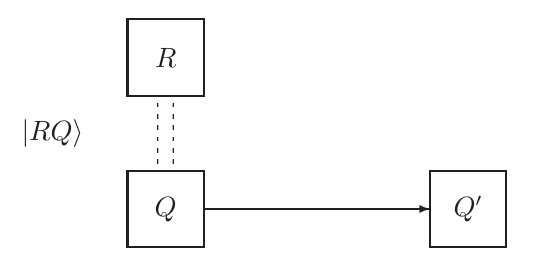
\includegraphics[width=0.5\textwidth]{images/entanglement-fidelity.png}
    \caption{The $RQ$ picture of quantum channel. The initial state of $RQ$ is a pure state.}
    \label{fig:entanglement-fidelity}
\end{figure}

How well is the entanglement preserved by the quantum operation $\mathcal{E}$ is described by \textit{entanglement fidelity} $F(\rho, \mathcal{E})$ which is defined for trace preserving operations $\mathcal{E}$ by
\begin{align}
    F(\rho, \mathcal{E}) &\equiv F(RQ, R'Q')^2 \\
    &= \bra{RQ} \left[ (\mathcal{I}_R \otimes \mathcal{E}) (\op{RQ}) \right] \ket{RQ}
\end{align}
where prime implies after the operation. Entanglement fidelity close to $1$ implies well preserved state and vice versa. One of the important properties of entanglement fidelity is that there's a nice formula to calculate it exactly. Suppose $E_i$ is a set of operation elements for $\mathcal{E}$. Then
\begin{align}
    F(\rho, \mathcal{E})  = \bra{RQ} \rho^{R'Q'} \ket{RQ} = \sum_i |\braket{RQ | E_i | RQ}|^2.
    \label{eq:letsoo}
\end{align}

Suppose $\ket{RQ} = \sum_j \sqrt{p_j}\ket{j}\ket{j}$, where $\rho = \sum_j \op{j}$. Then it can be proved that
\begin{align}
    \bra{RQ} E_i \ket{RQ} = \tr{E_i\rho}
\end{align}
Substituting this is equation \ref{eq:letsoo} we get a useful formula
\begin{equation}
    F(\rho, \mathcal{E}) = \sum_i | \tr{\rho E_i} |^2
\end{equation}

Surprisingly, these two notions are closely related too. This can be seen in two useful properties. First, the entanglement fidelity is a lower bound on the square of the static fidelity between the output and input to the process,
\begin{equation}
    F(\rho, \mathcal{E}) \leq \left[ F(\rho, \E{\rho} \right]^2
\end{equation}
This states that it's harder to preserve entanglement than it is compared to pure states. The second property is that it is a \textit{convex} function of $\rho$. i.e
\begin{equation}
    F\left( \sum_j p_j\rho_j, \mathcal{E} \right) \leq \Bar{F}
\end{equation}
This shows that any channel $\mathcal{E}$ which does a good job of preserving entanglement between a source system $\rho$ and reference system will automatically preserve  the ensemble source described by probabilities $p_j$ and states $\rho_j$ such that $\sum_j p_j\rho_j = \rho$.

I'll try to conclude with most important points yet.
\begin{enumerate}
    \item $0\leq F(\rho, \mathcal{E}) \leq 1$. From properties of static fidelity.
    \item Entanglement fidelity is linear in quantum operation input. This is immediate too.
    \item For pure state inputs, entanglement fidelity is square of static fidelity between input and output,
    \begin{equation}
        F(\qv, \mathcal{E}) = F(\qv, \E{\op{\psi}})^2.
    \end{equation}
    \item $F(\rho, \mathcal{E})=1$ if and only if for all pure state $\qv$ in support of $\rho$
    \begin{equation}
        \E{\op{\psi}} = \op{\psi}.
    \end{equation}
    \item Suppose that $\bra{\psi}\E{\op{\psi}}\qv \leq 1-\eta$ for all $\qv$ in support of $\rho$, for some $\eta$ then $F(\rho, \mathcal{E}) \geq 1-(3\eta/2)$.
\end{enumerate}
\part{Week 5}
\chapter{Entropy and information}
We know that \textit{entropy} measures uncertainity of state of a physical system. We'll look into it's definitions and properties deeply both in classical and quantum information theory.

\section{Shannon entropy}
It's the key concept of classical information theory. It can be viewed in two complementary views, first, suppose we have a random variable $X$, how much information we \textit{gain} on average if we know the value of $X$. Second, it's the measure of \textit{uncertainity} before we know the value of $X$.

Information content of a random variable doesn't depend on labels. For example, a random variaible giving `heads' and `tails' with probability $1/4$ and $3/4$ contains same information as a random variable giving `$0$' and `$1$' with probability $1/4$ and $3/4$ respectively. Thus, entropy also doesn't depend on labels. \textit{Shannon entropy} associated with a probability distribution $p_1,\dots,p_n$ is given by
\begin{equation}
    H(X) \equiv H(p_1,\dots,p_n) \equiv -\sum_x p_x\log p_x
\end{equation}
Note that by $\log$ we mean base $2$, by $\ln$ we mean base $e$. Since a never occuring event with probability $p_i=0$ should never affect entropy, thus we agree that $0\log 0=0$ even though we mean $\lim_{x\rightarrow0} x\log x = 0$. There's a nice reason why entropy is defined this way. We have to \textit{quantify the resources needed to store information}. Let's suppose a source producing symbols $X_1,X_2,\dots$ of independent \textit{identically} distributed random variables, minimal amount of resources required to store the information produced by source such that it can be reconstructed turns out to be just entropy i.e $H(X)\equiv H(X_1) \equiv H(X_2) = \dots$, this result is known as \textit{Shannon's noiseless coding theorem}.

I suggest looking at an example to understand this. Suppose our source produces $1$, $2$, $3$, $4$ which are symbols but with probability $1/2$, $1/4$, $1/8$ and $1/8$ respectively. We don't need two bits to store output of each use of source. We can compress this usage, by representing $1$ as $0$, $2$ as $10$, $3$ as $110$ and $4$ as $111$, with this we can reconstruct the message, for eg. $11010111$ as $324$ too. We need on an average $\frac{1}{2}\cdot 1 + \frac{1}{4}\cdot 2 + \frac{1}{8}\cdot 3 + \frac{1}{8}\cdot 3 = 7/4$ bits only! It also turns out that this is just the entropy of the source $H(X) = -1/2\log(1/2) - 1/4\log(1/4) - 1/8\log(1/8) - 1/8\log(1/8) = 7/4$. It's also true that average information gained by an event out of a probability distribution $p_1,\dots,p_n$ is $k\sum_ip_i\log p_i$ for some constant $k$.

\section{Basic properties of entropy}
\subsection{The binary entropy}
The entropy of a two-outcome random variable is so special that we name it as \textit{binary entropy}
\begin{equation}
    H_{\text{bin}}(X) \equiv -p\log p - (1-p)\log (1-p)
\end{equation}
where $p$ and $1-p$ are probabilities of outcome. It's graph is shown in figure  \ref{fig:binary-entropy} 
\begin{figure}
    \centering
    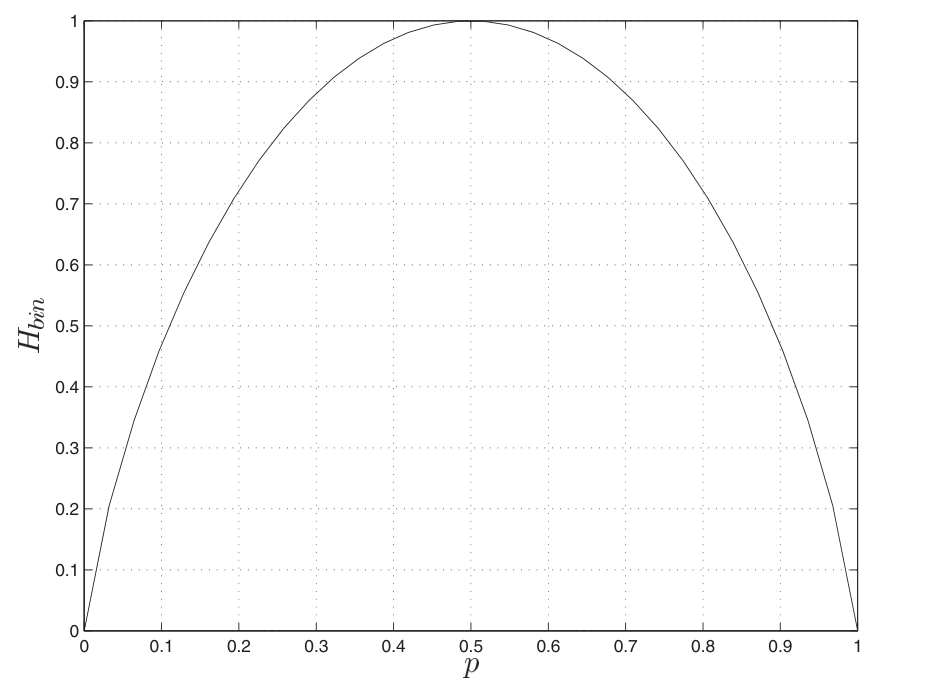
\includegraphics[width=0.65\textwidth]{images/binary_entropy.png}
    \caption{Binary entropy function $H(p)$}
    \label{fig:binary-entropy}
\end{figure}

A really good intuition comes when we consider this example of Alice having two biased coins one from US and another from Australia. Suppose the US coin gives head with probability $p_U$ and the Australian coin with probability $p_A$ and Alice flips one of those coins with probability $q$ for US coin and $1-q$ for Australian coin and she tells final `head' or `tail' to Bob. The information Bob gets is atleast the average information he gets from flipping one coin. Hence
\begin{equation}
    H(qp_U + (1-p)p_A) \geq qH(p_U) + (1-q)H(p_A)
\end{equation}
It's greater because Bob gets \textit{more} information about the country sometimes. For eg. if $p_U=0.1$ and $p_A=0.9$ and Alice says head, Bob would understand that it's more probable to be an aussie coin. This leads us into a very important property of entropy, \textit{concavity}. Which can be seen in binary case in the figure \ref{fig:binary-entropy}.

\subsection{The relative entropy}
The \textit{relative entropy} is useful entropy-like measure describing closeness of two probability distributions $p(x)$ and $q(x)$ over the same index set $x$, defined by
\begin{equation}
    H(p(x) \parallel q(x)) \equiv \sum_x p(x)\log \frac{p(x)}{q(x)} \equiv -H(X)-\sum_x p(x)\log q(x)
\end{equation}
The following theorem motivates us to understand it as a distance measure
\begin{theorem}[\textbf{Non-negativity of relative entropy}]
    The relative entropy is non-negative, $H(p(x) \parallel q(x)) \geq 0$ with equality if and only if $p(x)=q(x)$ for all $x$.
    \label{thm:non-negativity-of-rel-entropy}
\end{theorem}
The proof is simple using the definition of relative entropy and $\log x \ln{2} \leq x-1$ with equality only when $x=1$. Relative entropy itself is not very useful but used to study entropy, for example let $q(x)$ be uniform probability distribution over index set $X$ of size $d$ then for a probability distribution $p(x)$ over $X$, we have
\begin{equation}
    H(p(x)\parallel q(x)) = H(p(x)\parallel 1/d) = -H(X) - \sum_x p(x) \log (1/d) = \log d - H(X)
\end{equation}
and hence by theorem \ref{thm:non-negativity-of-rel-entropy} we have $\log d - H(X) \geq 0$ thus $H(X) \leq \log d$, a nice property hence a theorem!
\begin{theorem}
    Suppose $X$ is a random variable with $d$ outcomes. Then $H(X) \leq \log d$, with equality if and only if $X$ is uniformly distributed over those $d$ outcomes.
\end{theorem}

\subsection{Conditional entropy and mutual information}
For two random variables $X$, $Y$ we'll try to understand how information of $X$ is related to that of $Y$. First we define \textit{joint entropy} of $X$ and $Y$ as
\begin{equation}
    H(X, Y) \equiv -\sum_{x, y} p(x, y)\log p(x, y)
\end{equation}
The \textit{entropy of $X$ conditional on knowing $Y$} is similar to that in probability, it's the uncertainity that we have in the value of $X$ given that we know the value of $Y$. It's defined by
\begin{equation}
    H(X | Y) \equiv H(X,Y) - H(Y)
\end{equation}

A second quantity \textit{mutual information content of $X$ and $Y$} measures how much information $X$ and $Y$ have in common. It's very similar to intersection, given we take $H(X,Y)$ as information content of both $X$ and $Y$ which is counted twice. Thus, mutual information content is
\begin{equation}
    H(X:Y) = H(X) + H(Y) - H(X, Y)
\end{equation}
The relation $H(X:Y) = H(X) - H(X|Y)$ also comes in handy. Let's see some more simple relationships between different entropies.

\begin{ntheorem}[\textbf{Basic properties of Shannon entropy}]
    \begin{enumerate}
        \item $H(X, Y) = H(Y, X), H(X:Y) = H(Y:X)$
        \item $H(Y|X) \geq 0$ and thus $H(X:Y)\leq H(Y)$ with equality if and only if $Y$ is a function of $X$, $Y=f(X)$.
        \item $H(X) \leq H(X,Y)$ with equality if and only if $Y$ is a function of $X$.
        \item \textbf{Subadditivity:} $H(X, Y) \leq H(X) + H(Y)$ with equality if and only if $X$ and $Y$ are independent variables.
        \item $H(Y|X) \leq H(Y)$ and thus $H(X:Y) \geq 0$ with equality in each if and only if $X$ and $Y$ are independent distributions.
        \item \textbf{Strong subadditivity:} $H(X,Y,Z) + H(Y) \leq H(X,Y) + H(Y, Z)$, with equality if and only if $Z\rightarrow Y\rightarrow X$ forms a markov chain.
        \item \textbf{Conditioning reduces entropy:} $H(X|Y,Z) \leq H(X|Y)$.
    \end{enumerate}
\end{ntheorem}
All this can be easily understood by a Venn diagram for entropy.
\begin{figure}[H]
    \centering
    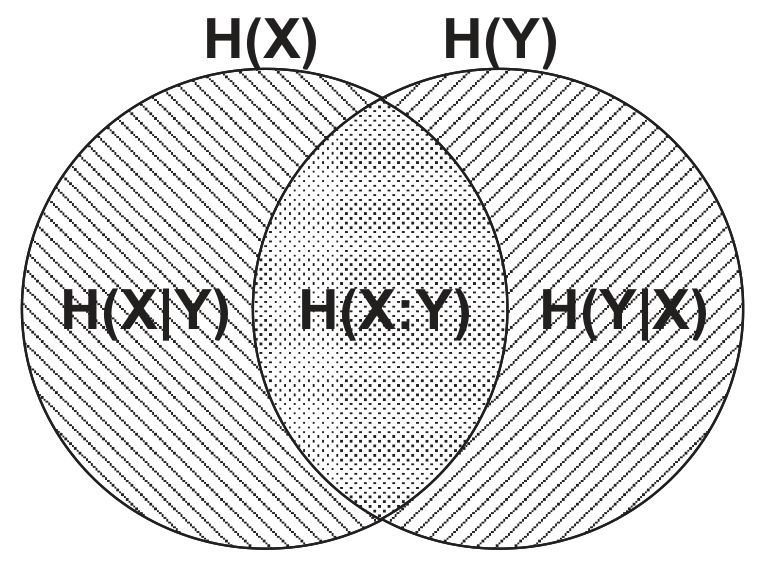
\includegraphics[width=0.45\textwidth]{images/venn_entropy.png}
    \caption{Relationships between different entropies}
    \label{fig:venn-entropy}
\end{figure}
Let's finally consider a simple and useful chaining rule for conditional entropies.
\begin{theorem}
    Let $X_1,\dots,X_n$ and $Y$ be any set of random variables. Then
    \begin{equation}
        H(X_1,\dots,X_n|Y) = \sum_{i=1}^n H(X_i|Y,X_1,\dots,X_{i-1})
    \end{equation}
\end{theorem}
\begin{proof}
    Use induction with base case $n=2$.
\end{proof}

\subsection{The data processing inequality}
This states that information from the output of a source can only \textit{decrease with time}; once information is lost, it's gone forever. The intuitive notion of \textit{information processing} is captured by \textit{Markov chanis} of random variables. A Markov chain is a sequence $X_1\rightarrow X_2 \rightarrow \cdots$ such that $X_{n+1}$ is independent of $X_1, X_2, \dots, X_{n-1}$ if $X_n$ is known. In other words
\begin{equation}
    p(X_{n+1}=x_{n+1} | X_n = x_n, %{X_{n-1} = x_{n-1}},
    \dots, X_1 = x_1) = p(X_{n+1}=x_{n+1} | X_n = x_n)
\end{equation}

\begin{theorem}
    Suppose $X\rightarrow Y \rightarrow Z$ is a Markov chain. Then
    \begin{equation}
        H(X) \geq H(X:Y) \geq H(X:Z).
    \end{equation}
    Moreover, this first inequality becomes equal if and only if, given $Y$, it's possible to reconstruct $X$.
\end{theorem}
This theorem is intuitive, as it says that if there's some noise introduced in $X$ (which leads to Markov chain $X\rightarrow Y$) then the mutual information between $X$ and $Y$ (which is what we want) is irretrievably lost, since it's not possible to reconstruct $X$ from $Y$ (noise).

If $X\rightarrow Y \rightarrow Z$ is a Markov chain, then so is $Z\rightarrow Y \rightarrow X$\footnote{Can be proved by using $P(X|Y)=P(X,Y)/P(Y)$}. Thus with above conditions, we see that
\begin{equation}
    H(Z:Y) \geq H(Z:X)
\end{equation}
This thing is also known as \textit{data pipelining inequality} i.e any information $Z$ shares with $X$ is also shared by $Y$. The information is \textit{pipelined} from $X$ to $Y$ to $Z$.

\section{Von Neumann entropy}
Shannon entropy is for classical probability distributions, Von Neumann defined this notion of \textit{entropy} for quantum state with density operator $\rho$ as 
\begin{equation}
    S(\rho) \equiv -\tr{\rho \log{\rho}}
\end{equation}
where $\log$ still means base $2$ and $0\log 0 \equiv 0$. This can be simplified if we know eigenvalues $\lambda_x$ of $\rho$ as
\begin{equation}
    S(\rho) \equiv -\sum_x \lambda_x \log{\lambda_x}
\end{equation}
This is very useful for calculations. We will refer \textit{entropy} to either Shannon or Von Neumann entropy based on context.

\subsection{Quantum relative entropy}
Similar to Shannon entropy, \textit{relative entropy} between two state $\rho$ and $\sigma$ is defined by
\begin{equation}
    S(\rho \parallel \sigma) \equiv \tr{\rho \log{\rho}} - \tr{\rho \log{\sigma}}
\end{equation}
as in classical case, this can sometimes shoot upto infinity. Particularly, relative entropy is defined to be $+\infty$ if the kernel of $\sigma$ (vector space spanned by eigenvectors of $\sigma$ with eigenvalue $0$) has non-trivial intersection with the support of $\rho$ (vector space spanned by eigenvectors of $\rho$ with non-zero eigenvalues). A familiar inequality as a theorem is given.
\begin{theorem}[\textbf{Klein's inequality}]
    The quantum relative entroy is non-negative. i.e
    \begin{equation}
        S(\rho \parallel \sigma) \geq 0,
    \end{equation}
    with equality if and only if $\rho=\sigma$.
\end{theorem}

\subsection{Basic properties of entropy}
These are few interesting properties of von Neumann entropy:
\begin{ntheorem}[\textbf{Basic properties of von Neumann entropy}]
    \begin{enumerate}
        \item The entropy is non-negative. The entropy is zero if and only if the state is pure.
        \item In a $d$-dimensional Hilbert space, entropy is atmost $\log{d}$. It's equal if and only if the system is completely mixed state $I/d$.
        \item If a composite system $AB$ is pure, then $S(A)=S(B)$.
        \item Suppose $p_i$ are probabilities and $\rho_i$ have support on orthogonal subspaces. Then 
        \begin{equation}
            S\left( \sum_i p_i\rho_i \right) = H(p_i) + \sum_i p_iS(\rho_i)
        \end{equation}
        \item \textbf{Joint entropy theorem:} Suppose $p_i$ are probabilities and $\ket{i}$ are orthogonal states for a system $A$, and $\rho_i$ is any set of density operators for another system, $B$. Then
        \begin{equation}
            S\left( \sum_i p_i\op{i} \otimes \rho_i \right) = H(p_i) + \sum_i p_iS(\rho_i).
        \end{equation}
    \end{enumerate}
\end{ntheorem}

Again similarly, the \textit{joint entropy} $S(A, B)$ for a composite system of two components $A$ and $B$ is defined obviously as $S(A, B) \equiv -\tr{\rho^{AB}\log{\rho^{AB}}}$, we also define conditional entropy and mutual information as
\begin{align}
    S(A|B) &= S(A,B) - S(B) \\
    S(A:B) &= S(A) + S(B) - S(A, B) \\
    &= S(A)-S(A|B) = S(B) - S(B|A). 
\end{align}

But there are some properties which aren't carried over from Shannon to von Neumann entropy. One such is $H(X,Y)\geq H(X)$ which is intuitive since we have more information if we know about $X$ and $Y$ compared to if we only know about $X$. But this isn't true for von Neumann entropy, consider a system $AB$ of two qubits in entangled state $(\ket{00}+\ket{11})/\sqrt{2}$. Since this is pure, $S(A, B)=0$. But it's component $A$ is $I/2$, and has entropy $1$ defying what we've seen above. Another way of seeing this is $S(B|A) = S(A, B) - S(A)$ is negative.

\subsection{Measurements and entropy}
We'll try to understand how measurements change the entropy of a system, if they do. This change ofcourse depends on the type of measurement we make. Suppose we do a projective measurement on system $\rho$ described by projectors $P_i$, the state of the system is
\begin{equation}
    \rho' = \sum_i P_i\rho P_i
\end{equation}
The following theorem shows the entropy never decreases
\begin{theorem}[\textbf{Projective measurements increase entropy}]
    Suppose $P_i$ is a complete set of orthogonal projectors and $\rho$ is a density operator. Then the entropy of the state $\rho' \equiv \sum_iP_i\rho P_i$ of the system after measurement is atleast as great as the original entropy,
    \begin{equation}
        S(\rho') \geq S(\rho)
    \end{equation}
    with equality if and only if $\rho' = \rho$.
\end{theorem}

\subsection{Subadditivity}
If two system $A$ and $B$ have a joint state $\rho^{AB}$. Then the joint entropy for the two systems satisfy
\begin{align}
    S(A,B) &\leq S(A) + S(B) \\
    S(A,B) &\geq |S(A) - S(B)|
\end{align}
The first relation is known as \textit{subadditivity} inequality\footnote{This can be proved simply using Klein's inequality.} for von Neumann entropy, with equality if and only if $A$ and $B$ are correlated, i.e $\rho^{AB}=\rho^A\otimes \rho^B$. Second one is known as \textit{triangle} inequality or \textit{Araki-Lieb} inequality. It's the quantum analogue of $H(X,Y)\geq H(X)$.

\subsection{Concavity of the entropy}
The entropy is a \textit{concave} function in its inputs. That is, given the probabilities $p_i$, and corresponding density operators $\rho_i$, entropy satisfies the inequality\footnote{To prove this we introduce an auxillary system $B$.}
\begin{equation}
    S\left( \sum_i p_i\rho_i \right) \geq \sum_i p_i S(\rho_i).
\end{equation}
A good intuition is that $\sum_ip_i\rho_i$ expresses a quantum state which is in an uncertain state $\rho_i$ with probability $p_i$, this uncertainity of index $i$ of state adds to the average uncertainity we have of each state $\rho_i$ which is $\sum_i p_iS(\rho_i)$. Equality holds if and only if all the states $\rho_i$ for which $p_i>0$ are identical; i.e, entropy is strictly concave in its inputs!

\subsection{The entropy of a mixture of quantum states}
The flip side of concavity is that it provides an upper bound of entropy of a mixture of quantum states too. It's shown by the following theorem.
\begin{theorem}
    Suppose $\rho=\sum_ip_i\rho_i$, where $p_i$ are some set of probabilities, and $\rho_i$ are density operators. Then
    \begin{equation}
        S(\rho) \leq \sum_i p_iS(\rho_i) + H(p_i),
    \end{equation}
    with equality if and only if the states $\rho_i$ have support on orthogonal subspaces.
\end{theorem}
This along with concavity completes our bound on entropy of a mixture of quantum states,
\begin{equation}
    \sum_i p_iS(\rho_i) \leq S\left( \sum_ip_i\rho_i \right) \leq \sum_i p_iS(\rho_i) + H(p_i).
\end{equation}
The intuition for this comes from the fact that we know too much information if we know on average about $\rho_i$ and $p_i$ also.

\section{Strong subadditivity}
This is an extension of subadditivity and triangle inequalities to three systems. The inequality states that for three quantum systems $A$, $B$, $C$,
\begin{equation}
    S(A, B, C) + S(B) \leq S(A, B) + S(B, C)
\end{equation}
\subsection{Proving strong subadditivity}
The proof is based on an important result, the \textit{Lieb's theorem}. For which, let's define few things. A function $f(A, B)$ which is a real-valued function of two matrices, is said to be \textit{jointly concave} in $A$, $B$ if for all $0\leq \lambda \leq 1$,
\begin{equation}
    f(\lambda A_1 + (1-\lambda)A_2, \lambda B_1 + (1-\lambda)B_2) \geq \lambda f(A_1, B_1) + (1-\lambda)f(A_2, B_2).
\end{equation}
Let's state Lieb's theorem now,
\begin{theorem}[\textbf{Lieb's theorem}]
    Let $X$ be a matrix, and $0\leq t \leq 1$. Then the function
    \begin{equation}
        f(A, B) \equiv \tr{X^\dag A^tXB^{1-t}}
    \end{equation}
    is jointly concave in positive matrices $A$ and $B$.
\end{theorem}
This theorem implies another theorem, convexity of the relative entropy.
\begin{theorem}[\textbf{Convexity of the relative entropy}]
    The relative entropy $S(\rho \parallel \sigma)$ is jointly convex in its arguments.
\end{theorem}
\begin{corollary}[\textbf{Concavity of the quantum conditional entropy}]
    Let $AB$ be a composite quantum system with components $A$ and $B$. Then the conditional entropy $S(A|B)$ is concave in the state $\rho^{AB}$ of $AB$.
\end{corollary}
This finally leads us to strong subadditivity.
\begin{theorem}
    For any trio of quantum systems $A$, $B$, $C$ the inequalities
    \begin{align}
        S(A)+S(B) &\leq S(A,C) + S(B,C) \\
        S(A,B,C) + S(B) &\leq S(A,B) + S(B,C)
    \end{align}
    hold.
\end{theorem}

\subsection{Elementary applications of strong subadditivity}
Strong subadditivity and related results have many useful applications in quantum information theory. Take the inequality $S(A)+S(B)\leq S(A,C)+S(B,C)$ which is true, it also holds for Shannon entropy too, but for different reasons. For practical applications strong subadditivity is most easily applied as a rephrasing in terms of conditional and mutual entropies. Here are three major reformulations
\begin{ntheorem}[\textbf{Reformulations of strong subadditivity}]
    \begin{enumerate}
        \item \textbf{Conditioning reduces entropy:} Suppose $ABC$ is a composite system. Then $S(A|B,C)\leq S(A|B)$.
        \item \textbf{Discarding quantum systems never increases mutual information:} Suppose $ABC$ is a composite quantum system. Then $S(A:B) \leq S(A:B,C)$.
        \item \textbf{Quantum operations never increase mutual information:} Suppose $AB$ be a composite system and $\mathcal{E}$ is a trace preserving quantum operation on $B$. Let $S(A:B)$ be before operation, $S(A':B')$ be after operation, then $S(A':B') \leq S(A:B)$.
    \end{enumerate}
\end{ntheorem}
We saw before that Shannon mutual information is not subadditive, thus quantum mutual information isn't subadditive either. But it turns out that conditional entropy is subadditive, i.e
\begin{equation}
    S(A_1, A_2|B_1, B_2) \leq S(A_1|B_1) + S(A_2|B_2)
\end{equation}
What's more, it's subadditive in the first and second entries.
\begin{theorem}[\textbf{Subadditivity of conditional entropy}]
    Let $ABCD$ be a composite of four systems. Then the conditonal entropy is jointy subadditive in the first two entries:
    \begin{equation}
        S(A,B|C,D) \leq S(A|C) + S(B|D)
    \end{equation}
    Let $ABC$ be a composite of three quantum systems. Then conditional entropy is subadditive in each of first two entries:
    \begin{align}
        S(A,B|C) &\leq S(A|C) + S(B|C) \\
        S(A|B, C) &\leq S(A|B) + S(A|C)
    \end{align}
\end{theorem}
We got introduced to relative entropy like a measure between density operators. It seems intuitive that this relative entropy decreases when we ignore a part of system is ignored, i.e it makes it harder to distinguish two states of that system and thus decrease any reasonable measure of distance between them. This following theorem states it:
\begin{theorem}
    Let $\rho^{AB}$ and $\sigma^{AB}$ be any two density matrices of a composite system $AB$. Then
    \begin{equation}
        S(\rho^A \parallel \rho^A) \leq S(\rho^{AB} \parallel \rho^{AB}).
    \end{equation}
\end{theorem}
\part{Week 6}
\chapter{Quantum circuits}
\section{Quantum algorithms}
Many interesting problems are impossible to solve on a classical computer, not because they're in principle insoluble, but because of the astronomical amount of resources they'd need. Quantum computing promises to enable feasible algorithms which would require unreasonably high resources for a solution on a classical computer.

As we've discussed before, two broad classes of quantum algorithms exist now, first is based on Shor's \textit{Quantum fourier transform} which provides \textit{exponential} speedup. Second is based on Grover's algorithm for performing \textit{quantum searching} which provides \textit{quadratic} speedup. Few main applications are listed in this figure
\begin{figure}[H]
    \centering
    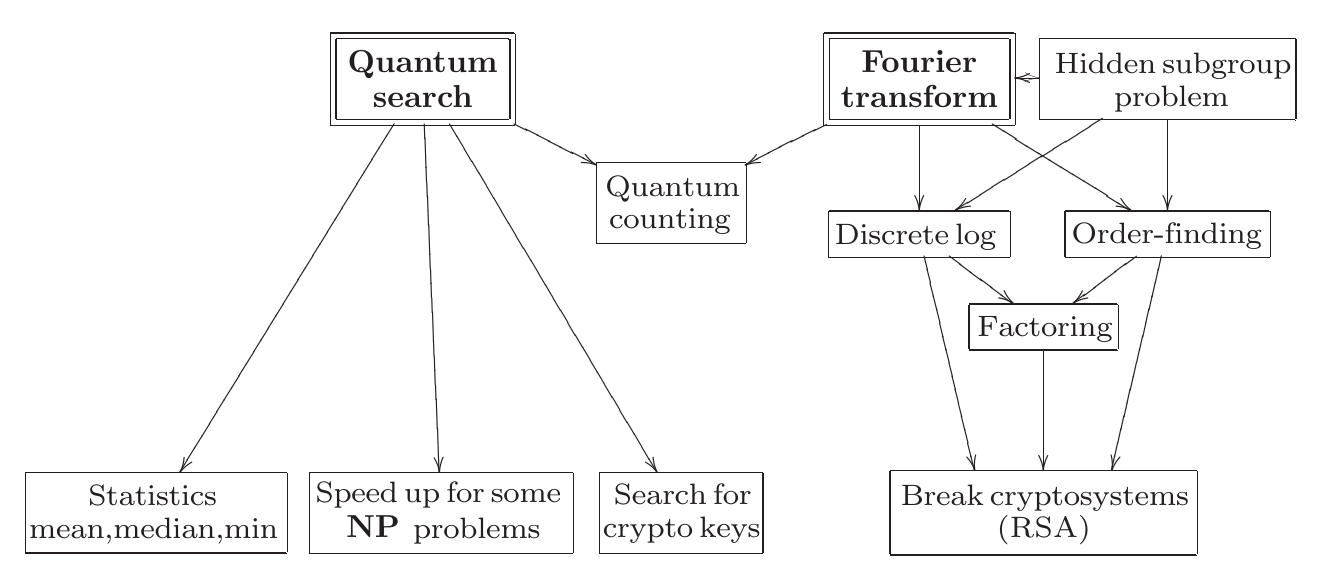
\includegraphics[width=0.9\textwidth]{images/quantum_algorithms.png}
    \caption{Main quantum algorithms with their applications and relationships.}
    \label{fig:quantum-algorithms}
\end{figure}

\section{Single qubit operations}
A single qubit is the simplest quantum system. We already know few important things like norm of the state is 1, operations on it are defined by unitary matrices etc. Few important gates/ operations are Pauli matrices ($I$, $X$, $Y$, $Z$) which we know. Three other important quantum gates are Hadamard gate ($H$), phase gate ($S$), and $\pi/8$ gate ($T$):
\begin{equation}
    H = \frac{1}{\sqrt{2}}\begin{bmatrix}
        1 & 1 \\ 1 & -1
    \end{bmatrix};
    \ \ \ 
    S = \begin{bmatrix}
        1 & 0 \\ 0 & i
    \end{bmatrix};
    \ \ \ 
    T = \begin{bmatrix}
        1 & 0 \\ 0 & \exp{(i\pi/4)}
    \end{bmatrix}.
\end{equation}
Few useful facts are $H = (X+Z)/\sqrt{2}$ and $S=T^2$, $T$ is known as $\pi/8$ gate instead of $\pi/4$ because it's equal to a gate with diagonal $\exp{(\pm \pi/8)}$ upto a global phase factor:
\begin{equation}
    T = \exp{(i\pi/8)}\begin{bmatrix}
        \exp{(-i\pi/8)  } & 0 \\ 0 & \exp{(i\pi/8)}
    \end{bmatrix}
\end{equation}
Also, in \textit{Bloch sphere} representation, the state $a\qo+b\qi$ can be represented as a point $(\theta, \varphi)$ where $a=\cos{(\theta/2)}$ and $b=e^{i\varphi}\sin{(\theta/2)}$, and the Bloch vector is $(\cos{\varphi}\sin{\theta}, \sin{\varphi}\sin{\theta}, \\ \cos{\theta})$.

Pauli matrices give rise to useful matrices when exponentiated, the \textit{rotation operators} about $\hat{x}$, $\hat{y}$ and $\hat{z}$ axes, defined by equations
\begin{align}
    % 1
    R_x(\theta) & \equiv e^{-i\theta X/2} = \cos{\frac{\theta}{2}}I - i\sin{\frac{\theta}{2}}X = \begin{bmatrix}
        \cos{\frac{\theta}{2}} & -i\sin{\frac{\theta}{2}} \\
        -i\sin{\frac{\theta}{2}} & \cos{\frac{\theta}{2}} 
    \end{bmatrix} \\
    % 2
    R_y(\theta) & \equiv e^{-i\theta Y/2} = \cos{\frac{\theta}{2}}I - i\sin{\frac{\theta}{2}}Y = \begin{bmatrix}
        \cos{\frac{\theta}{2}} & -\sin{\frac{\theta}{2}} \\
        \sin{\frac{\theta}{2}} & \cos{\frac{\theta}{2}}
    \end{bmatrix} \\
    % 3
    R_z(\theta) & \equiv e^{-i\theta Z/2} = \cos{\frac{\theta}{2}}I - i\sin{\frac{\theta}{2}}Z = \begin{bmatrix}
        e^{-i\theta/2} & 0 \\
        0 & e^{i\theta/2}
    \end{bmatrix} .
    \end{align}
this is because if $x\in \mathbb{R}$ and $A^2=I$, then $e^{iAx}=\cos{x}I+i\sin{x}A$. If $\hat{n}=(n_x,n_y,n_z)$ is real unit vector in three dimensions then generalize the rotation by $\theta$ about $\hat{n}$ by the equation
\begin{equation}
    R_{\hat{n}}(\theta) = e^{-i\theta \hat{n}\cdot \Vec{\sigma}/2} = \cos{\left( \frac{\theta}{2} \right)}I - \sin{\left( \frac{\theta}{2} \right)}(n_xX+n_yY+n_zZ),
\end{equation}
where $\Vec{\sigma}$ denotes the three component vector $(X, Y, Z)$ of Pauli matrices. A nice fact is that any unitary operator on a single qubit can be written as $U=e^{i\alpha}R_{\hat{n}}(\theta)$ for some $\alpha$, $\hat{n}$ and $\theta$. More generally

\begin{theorem}[\textbf{Z-Y decomposition for a single qubit}]
    Suppose $U$ is a unitary operation on a single qubit. Then there exist real numbers $\alpha$, $\beta$, $\gamma$, $\delta$ such that
    \begin{equation}
        U = e^{i\alpha}R_z(\beta)R_y(\gamma)R_z(\delta)
    \end{equation}
\end{theorem}
In general $z$ and $y$ can be replaced by any non-parallel real unit vectors $\hat{m}$ and $\hat{n}$. Also, this leads to a mysterious corollary, which'll be useful later.
\begin{corollary}
    Suppose $U$ is a unitary gate on a single qubit. Then there exist unitary operators $A$, $B$, and $C$ on a single qubit such that $ABC=I$ and $U=e^{i\alpha}AXBXC$, where $\alpha$ is some overall phase factor.
\end{corollary}
Here are few useful circuit identities:
\begin{equation}
    HXH = Z;\ HYH = -Y;\ HZH = X.
\end{equation}
also, $HTH=R_x(\pi/4)$. To recap things here are few quantum circuit symbols
\begin{figure}[H]
    \centering
    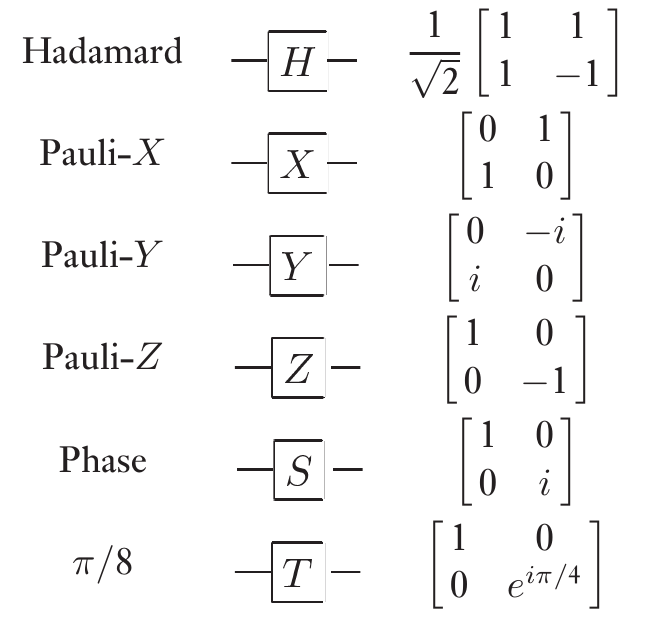
\includegraphics[width=0.4\textwidth]{images/circuit_symbols.png}
    \caption{Names, symbols and unitary matrices for commonly used quantum gates.}
    \label{fig:circuit-symbols}
\end{figure}
\section{Controlled operations}
`If $A$ is true, then do $B$' is the most useful and basic controlled operation in both classical and quantum computation. An example is \textsc{cnot} gate in quantum computation, which does $\ket{c}\ket{t}\rightarrow \ket{c}\ket{t\oplus c}$ where $\ket{c}$ is control qubit and $\ket{t}$ the target qubit. If $\ket{c}$ is in state $\qo$ nothing happens to target qubits, else if it's in $\qi$ $\ket{t}$ is flipped. A general thing for this is \textit{controlled-U} gate, which does $\ket{c}\ket{t}\rightarrow \ket{c}U^c\ket{t}$, where $U$ is a unitary operation. In the computational basis $\ket{\text{control, target}}$, the matrix representation of \textsc{cnot} gate is
\begin{equation}
    \begin{bmatrix}
        1 & 0 & 0 & 0 \\
        0 & 1 & 0 & 0 \\
        0 & 0 & 0 & 1 \\
        0 & 0 & 1 & 0
    \end{bmatrix}.
\end{equation}

To develop \textit{controlled-U} gate for arbitrary $U$, we'll use $U=e^{i\alpha}AXBXC$. To apply the controlled phase shift $\exp{(i\alpha)}$, we use a circuit containing a single qubit gate as shown
\begin{figure}[H]
    \centering
    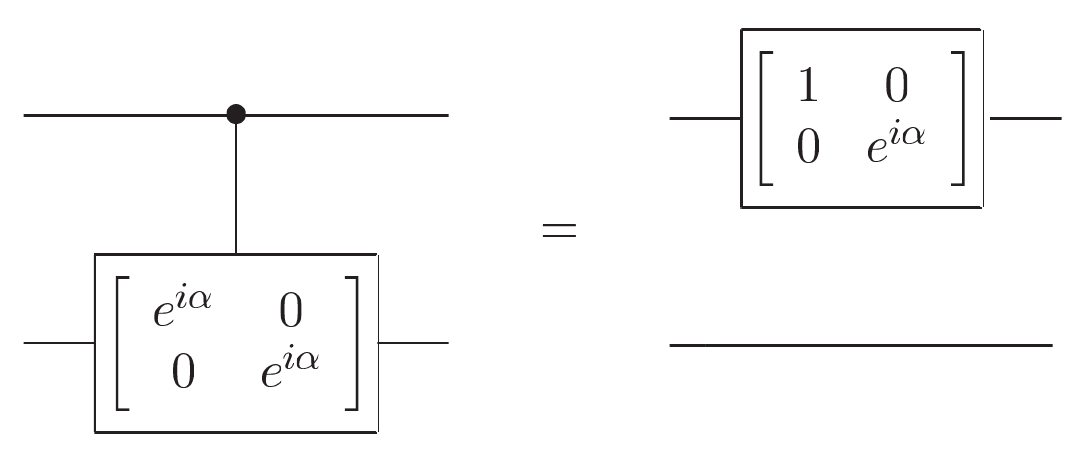
\includegraphics[width=0.5\textwidth]{images/phase_shift_circuit.png}
    \caption{Controlled phase shift gate and an equivalent circuit for two qubits.}
    \label{fig:phase-shift-circuit}
\end{figure}

To complete the gate we use the circuit \ref{fig:controlled-u-circuit}. This works because if control qubit is set to $\qo$ then nothing happens at \textsc{cnot} gates and $ABC=I$ is applied which does nothing, if control qubit is $\qi$ then $e^{i\alpha}AXBXC$ is applied, thus $U$ is applied. 
\begin{figure}[H]
    \centering
    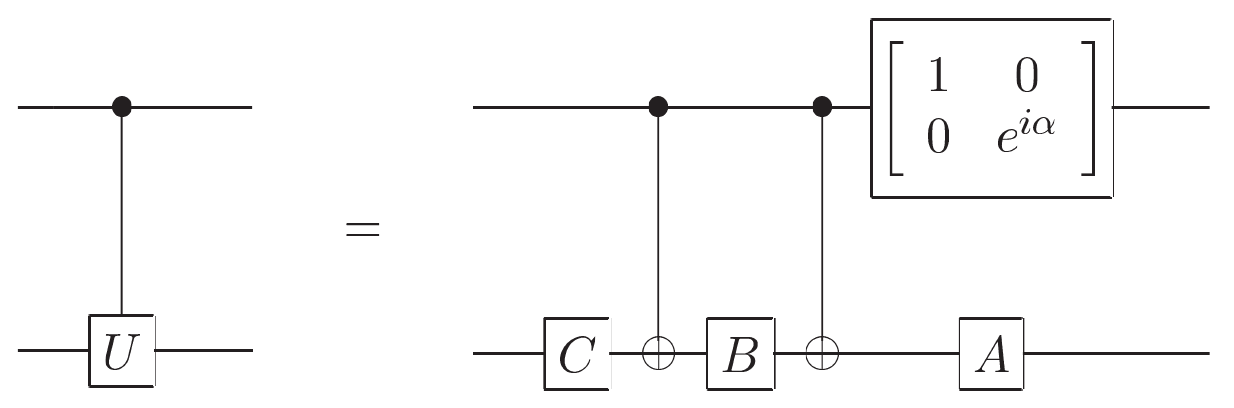
\includegraphics[width=0.7\textwidth]{images/controlled_u_circuit.png}
    \caption{\textit{controlled-U} circuit, $\alpha$, $A$, $B$, $C$ satisfy $U=e^{i\alpha}AXBXC$ and $ABC=I$}
    \label{fig:controlled-u-circuit}
\end{figure}

To use conditioning on multiple-qubits, suppose we have $n+k$ qubits, and $U$ is a $k$ bit operator. Then the controlled operatioin $C^n(U)$ by the equation
\begin{equation}
    C^n(U)\ket{x_1x_2\dots x_n}\qv = \ket{x_1x_2\dots x_n}U^{x_1x_2\dots x_n}\qv
\end{equation}
where $x_1x_2\dots x_n$ means product of those bits. It means operation $U$ is applied on last $k$ qubits if all of the first $n$ qubits are $\qi$. We'd assume $k=1$, for $k\geq2$ we don't yet know how to perform $k$ arbitrary operations at once.
\begin{figure}[H]
    \centering
    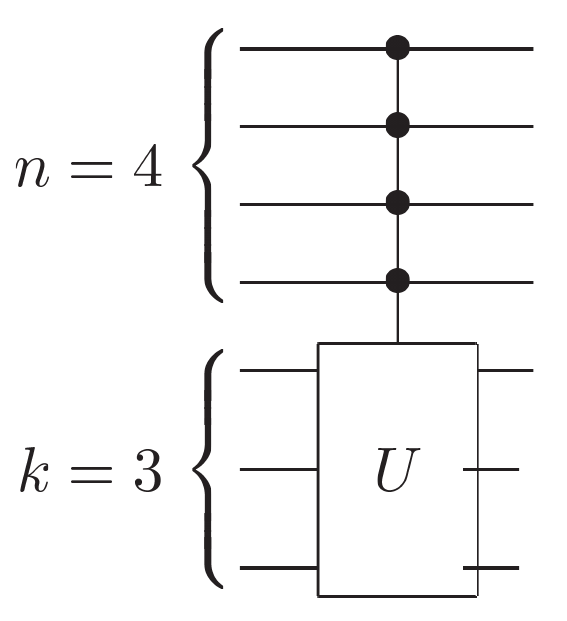
\includegraphics[width=0.4\textwidth]{images/multi_qubit_operation_circuit.png}
    \caption{$C^n(U)$ operation for $n=4$ and $k=3$.}
    \label{fig:multi-qubit-operation}
\end{figure}

\end{document}